% **************************** define graphics path **************************
\ifpdf
    \graphicspath{{chapter5/figs/raster/}{chapter5/figs/pdf/}{chapter5/figs/}}
\else
    \graphicspath{{chapter5/figs/vector/}{chapter5/figs/}}
\fi

\chapter{what do you mean?! the predictive power of vocabulary manipulation for abuse detection}\label{chap:liwc}
\chaptermark{what do you mean?!}

one of the key issues in machine learning for content moderation is that such systems both in deployed settings (see \cref{chap:filter}) and in research (see \cref{chap:intro} and \cref{chap:nlp}) over-fit to individual tokens that see over-representation in the positive and negative classes respectively.
similarly, efforts in nlp have identified that content moderation systems are likely to over-fit to identity markers such as the mentions of gender and race \citep{dixon:2018}.
while research efforts have been made to address such issues, the problem of over-fitting to words and identity markers remain an open question for the field.
although some such approaches have addressed this problem by replacing certain words and phrases to balance identity distributions \cite{dixon:2018}.
in this chapter, i propose a different approach which serves to address the issue of models over-fitting to tokens by 1) minimising the size of the vocabulary in order to avoid over-fitting to distributional skews of low-frequency tokens across classes; 2) representing documents in terms of how they serve as a proxy for thoughts, feelings, and personality; and 3) through such vocabulary minimisation highlight the importance of the mental and emotional states communicated, rather than the surface form of tokens while retaining model performance.
an additional benefit of such vocabulary reduction is a reduction in model size and optimisation time for complex models such as neural networks, resulting in models that have a smaller environmental impact \citep{strubell:2019}.
\ztedit{thus in this chapter, i seek to provide an answer to \textit{rq ii} by asking \textit{rq 2}: what are the modelling implications of using the linguistic inquiry and word count (liwc) resource to substitute the use of words and sub-words as input tokens?}

through this use of liwc \cite{pennebaker:2015,pennebaker:2001}, i pre-process documents from large vocabularies, that are riddled with obfuscations and intentionally and unintentionally misspelled words into a smaller vocabulary set representing instead psycholinguistic properties of words.
through a reduction of thousands, or in some cases hundreds of thousands, of unique tokens to hundreds of liwc categories, i aim for models to gain deeper insight into language patterns of abuse than simply selecting the most frequently used tokens.
moreover, i show that such a reduction is accompanied by a negligible reduction in intra- and inter-dataset performance in comparison to models using the full surface-token vocabularies.

through the use of simple deep neural networks and `shallow' linear models, i show that by reducing the vocabulary sizes by up to $98.0\%$ and the number of model parameters by up to $98\%$, while increasing the depth of the information in the remaining vocabulary, it is possible to achieve comparable performances within datasets and, in some cases, improvements on out-of-domain datasets. 
this holds two strong implications for future research on computational hate speech detection: first that current approaches through an over-reliance on surface forms are computationally inefficient, and second that the exclusive use of surface forms of tokens can lead models to overly attend to the occurrence of certain tokens and variations (e.g. prominent misspellings) \citep{rottger:2021}.
finally, as datasets for hate speech detection frequently contain biases along racialised and dialectal lines \citep{waseem:2018,davidson:2019}, the use of liwc can serve as small, but conflicted aid in avoiding such biases as dialectal spellings of words are likely to not appear in the dictionary, thus being relegated to unknown tokens (see \cref{tab:liwc_tok} for synthetic examples of liwc representations).

\section{previous work}

in the interest of curtailing the spread of online abuse, a large number of technical approaches have been considered in the ever-increasing body of research on the topic (please see \cref{chap:nlp} for a broad overview on the topic).
here, i focus on three different strands of research. 
first, i briefly introduce the liwc dictionary. 
second, i consider manual development of features for machine learning models, as it is necessary to form hypotheses for what might serve as indicators of abuse, on the basis of the dataset and problem in question.
third, i examine neural network approaches for abusive language detection.
finally, i consider the growing body of research devoted to examining the generalisability of computational models for abusive language detection. 
i restrict my attention to studies in conducted on abuse in english as it is most pertinent to this work.

\subsection{linguistic inquiry and word count}

the linguistic inquiry and word count dictionary and software was initially developed by \citet{pennebaker:2001} in an effort to address the issue of high disagreement and negative effects on well-being of judges, as they reviewed essays written on people's experiences of emotional upheaval. 
in order to minimise such costs, \citet{pennebaker:2001} turned to computationally counting words that were in $80$ ``psychology-relevant categories'' in order to gain an understanding of the emotional states and cognition of the speakers at the time of writing.
by passing over a large body of text within a single document, e.g. personal essays, \citet{pennebaker:2001} compute the percentage occurrence of each invoked category.
while there are some examples that appear clear cut, e.g. the categorisation of articles such as `a' and `the', other word classes, such as ``emotion word categories'' are more clearly subjective and require deeper human consideration \citep{tausczik:2010}.
though liwc was initially developed using long form texts, the version of the dictionary that i use in this dissertation is an expanded version that also used twitter and ``blogs'' in the development of the dictionary \citep{pennebaker:2015}.
as such, though not originally intended for the use on short-form messages, liwc has evolved with the rise of new forms of communication in efforts for the dictionary to accurately reflect language use in short-form documents.
as liwc was originally developed using long-form documents in the united states of america, the language that is reflected in the dictionary is predominately white american english and thus it excludes other languages and many dialects within american english.
by such exclusion, the dictionary does not accommodate for different forms of communicating, in particular it is likely to only insufficiently cover the language use of a variety of marginalised communities.
such a lack of recognition however has a benefit.
by not learning language patterns of e.g. african american english speakers who are disproportionately represented in the positive classes of several datasets for abuse \citep{waseem:2018,davidson:2019}, it is possible that models optimised on this representation are less likely to be biased against those groups.
although such lack of recognition can have positive effects, such as lower false positive rate, the politics of not being recognised, as argued by \citet{benjamin:2019} are not straightforward and the lack of recognition does not provide a guarantee that systemic harm will not occur.
for instance, if systems developed to detect abuse did not recognise multi-cultural london english due to vocabulary reductions, any abuse that was written in that dialect would not be recognised, leaving those users in harms way.
given that liwc was developed using ``dictionaries, thesauruses, questionnaires, and lists made by research assistants'' \citep{tausczik:2010} in a north american context, it is highly unlikely that word forms that differ from mainstream usage were included.
for instance, the commonly used `brotha' and `bruva' in north american and british contexts, respectively, are absent from the dictionary.
\vspace{5mm}

in this thesis, i utilise liwc to provide the word categories that each word invokes, and rather than compute the overall word classes exhibited in a document, i use the liwc categories of each word in a document as an alternative representation of the document from which percentages of word categories invoked can be recovered.
thus, my approach diverges slightly in the goals of using liwc, however it does not diverge in the method for obtaining information about the psychological state of the speaker.

\ztedit{
\subsubsection{limitations of psychometrics}
the use of psychometrics for computational research is a highly contested practice that has been used in highly concerning cases, notably psychometrics were used by cambridge analytica in their electoral campaigns \citep{stark_2018}.
in their paper ``algorithmic psychometrics and the scalable subject'', luke \citet{stark_2018} highlights the racist, sexist, and classist history of psychometrics, which were originally proposed by francis galton, a known eugenicist \citep{stark_2018}.
psychometrics were first proposed as ``the art of imposing measurement and number upon operations of the mind'' (francis galton quoted in \citet{stark_2018}), which aligned with galton's views on eugenics as methods for psychometrics were amenable to ``hierarchies of class, race and sex in victorian britain's industrial imperialist capitalism'' \citep[p.209]{stark_2018}.
rather than steering away from this troubled past, the field of psychometrics has continued to embrace the foundational notions proposed by galton and begun to operate in digital media on large bodies of data.
however, as \citet{stark_2018} argues, the use of psychometrics to make judgements on and for people faces a serious challenge of the ongoing development of people as they lack both qualitative and quantitative data about a whole person.

liwc, as a psychometric tool is embedded within this troubling history and development.
in particular, being a mixture of statistical correlations and human judgements liwc comes to embody the particular subjectivities of the developers of the dictionary.
this is particularly evident in its lack of inclusion of terms that are particular to dialects within and outside of the united states of america.
the creators of liwc indeed caution a heavy reliance on the dictionary as a means to identify the mental and emotional states, arguing that it is in nature imprecise \citep{tausczik:2010}.

in the work described below, there is a heavy reliance on liwc, however it is not used to predict the emotional and mental states of the speakers of given texts.
instead, i use it precisely because of its impreciseness and its highly limited expression, to gain a very rough alternate representation to the texts provided.
while this limited expression does not allow for making judgements on the mental states of the speakers, it does allow for an investigation into the potential of representing texts for abuse classification using a smaller vocabulary that does not rely on the structured (i.e. part of speech tags) but instead provides a rudimentary approximations of speakers' subjectivities.
}

\subsection{modelling}
\subsubsection{manually selected features}

a large body of work has sought to use manually developed features for online abuse detection \citep[e.g.]{davidson:2017,waseem:2017,wiegand:2019,fortuna:2018}, showing performance boosts from using manually developed features such as the predicted speaker gender \citep{waseem-hovy:2016} or part-of-speech (pos) tags \citep{davidson:2017}.
the primary reasons for using manually crafted features is two-fold: first, by using manually crafted features it is necessary to have some understanding of the data at hand and some intuition about which features may distinguish the classes in the data from one another. 
second, as manual features are frequently used with models that don't use neural architecture, they allow for interpretable models, in the sense that one can often identify how each token contributed towards a final prediction. 
moreover, as features are often computationally fast to compute, the use of features along with their expressive interpretability, allow for quickly testing hypothesis surrounding online abuse and its nature.
in a consideration of a handful of systems that employ some of the most frequently used features for the development of automated systems for detecting various forms of online abuse, distinct modelling choices, features and rationales for their use become prominent.
here i provide a brief overview of prominent features; how they are used, including which models and feature weighting schemes they are used with; and the explicit and implicit rationales for the use of each feature.

first, the most common feature used, and rarely used on its own, is a bag-of-words (bow) \citep{fortuna:2018,davidson:2017}, where each token in a document is treated as independent from the remainder of the document. 
the use of this feature frequently relies on the use of stop-word lists to remove tokens that are bound to occur frequently across a majority of documents, such as determiners, to avoid models from learning spurious correlations with such words and an individual class due to fluctuations in the data. 
the understanding of abuse that underlies this feature, is that the occurrence of some tokens are likely to disproportionately occur in abusive contexts, and that those tokens, in isolation, will indicate abuse. 
several works have complicated this notion \citep[e.g.]{waseem:2018,davidson:2019}, arguing that tokens, in isolation, do not provide the necessary context to determine whether a text is abusive.
due to certain perspectives on abuse being overly represented \citep{waseem:2016} in annotation guidelines and annotations, some words that have been reclaimed, and thus have an innocuous usage potentially in addition to an abusive use, may be disproportionately represented in the positive classes.

to address the issue of token independence, several approaches use n-grams, often bi-grams \citep{waseem:2016} and tri-grams \citep{davidson:2017} to aid with identifying abuse. 
here, by considering groups of sequential token occurrences independently from one another, a step is taken away from the independence of individual tokens, instead to the independence of short sequences of tokens. 
due to this remaining independence assumption, similar issues arise to the limitations of bow hold for n-grams.

pos tags have also seen frequent use in abusive language detection tasks \citep{fortuna:2018} and are often used as n-grams. 
the intuition behind the use of pos tags for abuse detection is that abuse may differ from non-abuse in terms of linguistic structure. 
while n-grams of pos tags with an independence assumption may not reveal the full depth of the linguistic syntax available through pos tagged data (in contrast to the pos tags of the entire sequence being treated as a single feature), it does relay \textit{some} information on the linguistic structure which has been proven helpful for predicting abuse \citep{fortuna:2018}.

another frequently used feature is sentiment analysis \citep{fortuna:2018} with the underlying assumption that abuse and negative sentiment are correlated, and can thus aid in detecting some forms of abuse.
similarly to bow and n-grams, this is a feature that is most frequently used in combination with other features as sentiment alone is not presumed to be a good predictor of abuse \citep{fortuna:2018}.
sentiment as a feature, like the use of liwc proposed in this dissertation, assumes that some more abstract reasoning about the data can be helpful to automatically detecting abuse.
specifically, its use suggests that there the concepts of negativity and hostility towards entities will be relevant to detecting abuse in texts.
some previous work that uses sentiment as a feature for abuse detection \citep{davidson:2017} relies on off-the-shelf systems for detecting sentiment and may therefore not be attuned to how sentiment and abuse interact.
an implication of using off-the-shelf systems for computing sentiment, rather than assuming that sentiment can be extrapolated only from a mapping of the occurrence of abuse to sentiment, is that sentiment and abuse, while correlated are not equated and thus that the task of detecting sentiment, while related is a distinct task from detecting abuse.
as such, sentiment and abuse detection are tasks that in some cases co-constitute each other while there may be no correlation in other cases.

finally, liwc has previously been proposed as a feature for the classification of abuse in a small number of studies \citep{nina:2018,joksimovic:2019}.
in these studies, liwc has been used in conjunction with other features such as lexical features (e.g. word n-grams) and syntactic features (e.g. pos tags) \citep{joksimovic:2019}.
this use of liwc, similar to the motivations for its use in this chapter, relies on an assumption that the mental states of the speaker and the interpretations of readers will relay information on the intention of the speaker to cause offence.
for instance, \citet{nina:2018} compute the percentages of emotions that are expressed in abusive documents in efforts to identify correlations between impassioned speech and abuse, asserting an intuition that abusive speech is likely to occur in individual moments dominated by emotion rather than rationality.
a position that \citep{waseem:2016} argue is likely as they find that considering the top $100$ most frequently occurring tokens, ranked using term frequency - inverse document frequency (tf-idf), does not aid in the prediction of hate speech, suggesting that in many cases it may be a question of moments of abuse rather than consistently abusive people.

all features must be weighted, either through raw counts or their relative frequency.
one such frequently used weighting scheme is tf-idf which weights features by their relative frequency in the corpus \citep{fortuna:2018}, assigning higher weight to the features that are rare corpus-wide and lower weights to those that common.
as such, tf-idf can be a useful measure to address the dominance of high-frequency tokens.
at the same time, tf-idf also increases the capacity for models to over-fit to the corpus and generalise poorly, as tokens that are unique to a corpus may not exist in other data or even be common to other data.
the use of n-grams as features provides a similar double-edged benefit, where models learn sequences of words.
in abuse detection the most common n-grams are unigrams, bi-grams, and trigrams.
such word-sequences can be helpful for models in uncovering patterns of language use in the corpus but are also vulnerable to vocabulary changes that occur across datasets.
for instance \citet{waseem-hovy:2016} optimise a logistic regression classifier and identify that character n-grams of innocuous words such as `islam' and `muslim' rank as some of the most predictive features due to the disproportionate occurrences of such terms in the hateful classes.

many of the previously mentioned works use similar machine learning models, with a particular dominance of logistic regression and support vector machines (svms) (please see \cref{chap:nlp} for more detail).
one notable exception to this is the work of \citet{gorrell:2018}.
in this work, the authors use a ``set of nlp tools, combining them into a semantic pipeline'' \citep[pp. 601]{gorrell:2018}.
rather than using supervised classification techniques, a rule-based systems was developed to detect abuse that they argue allows for a interpretable and easy to modify method to address weaknesses of the approach without the need for additional large quantities of data.\footnote{this detail on the rule-based nature of the classification systems was provided by genevieve gorrell in personal communications.}
however, this approach is a laborious one as it requires the researchers to manually identify patterns of abuse and construct rules that can address such patterns along with any exceptions to the patterns that are not abusive.

\ztedit{
\paragraph*{prior work on lexical replacements}
}
\ztedit{
  reducing the dimensionality of data has been approached from a number of different avenues in prior literature.
  a large body of work is dedicated to the mathematical induction of what features to retain and which to omit\citep{...}.
  the object of the mathematical approach is to identify which features provide the most information about the distinctions between each class and which features provide the least information, and therefore can be omitted when optimising a machine learning model.
  another body of work has been dedicated to dimensionality reduction through semantic replacements.
  one approach to such a reduction is the use of clustering algorithms, e.g. brown clustering \citep{derczynski_2015}.
  another, more recent approach is to perform partial replacements of some tokens.
  this method has been used in recent studies on abuse detection by using the hurtlex resource \citep{bassignana_basile_patti_2018}.
  hurtlex is a multi-lingual lexicon that seeks to map ``offensive'' words into three macro categories, and seventeen fine-grained categories.
}

\ztedit{
  several papers have approached the task of abuse detection across multiple languages by using hurtlex to perform a reduction in the feature space of offensive words in the lexicon.
  for instance, \citet{pamungkas_2020} use hurtlex to create a feature vector for each of the fine-grained categories to be used for training and classification, as a way to separate out profanities and hateful terms.
  \citet{chiril_2019} use hurtlex across english and french tweets to count the number of times each of the fine-grained categories are invoked.
  they optimise their models using the length of the tweets along with the number of times each fine-grained category is invoked in a tweet.
  others have used hurtlex in combination with deep learning methods by creating onehot encodings \citep{pamungkas_2019} and using the encoding to create a hurtlex embedding layer \citep{koufakou_2020}.
  these approaches all either directly reduce the feature space or seek to force optimised models to pay particular attention to the tokens included in the hurtlex resource.
  the approach that i take in this chapter contrasts these approaches by replacing all tokens with their respective liwc categories and optimising models on the resulting document representations.
}

\vspace{5mm}

in this chapter, i take inspiration from the use of manually crafted features as a way to provide testable hypothesis while departing from the notion of feature generation.
specifically, i hypothesise that liwc categories can provide deep information for predictive modelling that can allow for high performance in spite of token sparsity when using neural network methods.

\subsubsection{neural networks}\label{sec:liwc_nn}
though the earliest models for the tasks were predominately linear models that used manually generated features \citep{waseem-hovy:2016,davidson:2017,warner:2012} more recent work has been dominated by the development of neural network based models for automated abuse detection, posting ever-evolving state-of-the-art models and classification performances \citep[e.g.]{park:2017,badjatiya:2017,zimmerman:2018,stoop:2019,isaksen:2020}.
here i consider a handful of neural network methods for detecting abuse, focusing on the distinct implications following the modelling choices and the logics that underpin them.
as all neural network based methods that i examine receive only the text as input, the primary differences between the models is in their use and organisation of different types of layers and the loss function selected for the respective models.

the most commonly used architecture for neural networks that in the surveyed literature is a cnn \citep{park:2017,gamback:2017,wulczyn:2017,kolhatkar:2020,zimmerman:2018,wang:2020}.
as cnns have been the subject of particularly interest, a number of distinct modelling approaches have been proposed.
first, relying on a simple neural network architecture, \citet{kolhatkar:2020} use glove embeddings as the first layer, followed by three convolutional layers (that have window sizes $3, 4,$ and $5$, respectively) with global maximum pooling layers.
prior to passing to an output layer, dropout is applied to the output of the convolutional layers which is then passed to a dense layer.
all layers prior to the output layer use a relu (see \cref{chap:nlp} for more detail) activation function.
the output layer applies the sigmoid function to provide a prediction from the model.
this model most closely resembles the cnn architecture used in this chapter.
as this model uses a pre-trained word-embedding layer as its input layer, the input the model receives are documents that have been subject to tokenisation processes.

a different architecture is proposed by \citet{park:2017}.
in their work they compare a single classifier, what they dub a `one-step classifier', that predicts the final classes directly with a stacked architecture of two models, or a `two-step classifier' in their vernacular, that first predicts whether content is abusive and second predicts which type of abuse the documents predicted as abusive are.
there are two primary distinctions between the two-step architecture proposed by \citet{park:2017} and the architecture proposed by \citet{kolhatkar:2020}.
first, \citet{kolhatkar:2020} acts as a one-step classifier whereas the architecture proposed by \citet{park:2017} acts in two steps.
second, \citet{kolhatkar:2020} only acts on documents tokenised into words and punctuation whereas \citet{park:2017} propose a cnn that takes documents tokenised into words and punctuation in addition to documents tokenised into characters.
\citet{park:2017} show that through the use of a one-step cnn optimised on word and character input, they achieve a performance boost obtaining a f1-score of $0.827$ on the datasets proposed by \citet{waseem-hovy:2016} and \citet{waseem:2016}, though the performance boost is lost once a two-step hybrid cnn is used.

as cnns build feature mappings by passing over the data using filters, they come with certain assumptions built into them.
as researchers define the number of filters and the stride size, they also define the range, in terms of token order, within which the is given leave to identify token interactions.
the implication of this is then that there will likely be some, potentially overlapping, ranges that the models learn patterns from.
depending on how researchers define these, the models will develop feature mappings corresponding to the ranges provided.

another frequently used architecture is lstms \citep{badjatiya:2017,kolhatkar:2020,meyer:2019}.
for instance, \citet{kolhatkar:2020} propose using a bi-directional lstm that, like their cnn, has a pre-trained embedding layer, a recurrent layer, a dropout layer, and a fully connected output layer with a sigmoid activation to predict the output classes.
\citet{meyer:2019} on the other hand take develop on the idea of a hybrid cnn, developing a lstm architecture that takes documents tokenised into words and characters as input.
the word representation is obtained through tokenisation passed through an embedding layer and the character representation is obtained by processing the documents with a cnn.
using these approaches, \citet{kolhatkar:2020} show comparable performances between the cnn and bi-directional lstm on their dataset.
\citet{meyer:2019} on the other hand show that a baseline model only using character level information performs comparably with other more complex approaches, obtaining a macro f1-score of $0.7923$ for the baseline and $0.7924$ for the final system on the dataset proposed by \citet{waseem-hovy:2016}, and notably out-performs several other previously proposed methods.

the use of lstms, that rely on recurrence, break with the independence assumption of the manual feature-based models.
by recurring over a document, each new token is considered in conjunction with the previous tokens that have not been forgotten.
in this way, an assumption is built into the models that through processing enough token sequences, it will be possible to identify patterns in the sequences of tokens that connote abuse.
such a reliance on the text alone does not consider the positionality of abuse; \citet{waseem:2018} argue only through understanding the context within which the speaker and audience exist in, is it possible to deem something as abusive.
for instance, it is only through an understanding of the speaker that one can deem whether the \textit{n-word} is weaponised as abuse or is reclaimed to connote complex social identity.
\vspace{5mm}

all methods described that rely on documents tokenised into sentences rely on pre-trained embedding layers (most frequently glove \citet{pennington:2014}) that come with their own benefits and costs.
for instance, word embeddings that are optimised on web-text are likely to harbour social biases \citep{bolukbasi:2016} that have been proven hard to address \citep{gonen:2019}.
on the other hand, they also allow for better representations of related concepts and will be less susceptible to creating different representations for closely related concepts as a result of dataset biases.
for instance, the concepts `television' and `t.v.' might only be distantly related, if at all, in a small dataset due to few co-occurrences within the dataset.
in a larger dataset, spanning millions of documents, these two concepts are likely to appear as closely related as a robust language representation will likely have been achieved for such commonly occurring tokens.
the methods that rely on character embeddings are also subject to similar distributional concerns, however this can be a benefit when used in conjunction with word embeddings.
this benefit comes through as the set of possible characters is much smaller than the set of possible unique words, less data is needed to optimise robust embedding layers, though the optimised character embeddings will be particularly attuned to the dataset at hand.
on the other hand, due to such particularity of the character embeddings, they are less likely to map well onto other domains even if they show good performance on the dataset that they are derived from.
\vspace{5mm}

for the work in this chapter, the use of pre-trained embeddings is not appropriate for some models.
specifically the models that use liwc-represented documents as liwc embeddings are not publicly available or have been developed, to the best of my knowledge.
moreover, documents represented through liwc categories are poorly suited for optimising general embeddings as only a small set of tokens are defined and they are not necessarily distributed in a fashion suitable for developing such generalised  embeddings.
second, i don't use pre-trained embeddings in the architectures for all other models to ensure that any comparisons with the liwc-based models are a direct comparison of the influence of using liwc as input tokens and avoiding potentially confounding factors.

\subsection{datasets}\label{sub:liwc_datasets}
in order to understand and validate my approach, i optimise a model on multiple datasets.
moreover, i take each model that is learned on a given dataset and apply it to all other datasets.
to accommodate prediction on a model optimised on one dataset to others, i reduced all classification tasks to a binary task of abusive and not-abusive.
this has downstream implications for the construction of the datasets and for the validity of the prediction task on the auxiliary datasets.
first, the dataset distributions are modified as tasks with more than two classes see their data collapsed. 
for some datasets, this means that the class imbalances are improved, as the majority class is non-abusive.
the exception to this is the dataset proposed by \citet{davidson:2017} where the largest class is the `offensive' class, which i combine with `hateful', further minimising the relative size of the negative class.
second, as each dataset has been collected with different rationales and annotated with distinct purposes (please see \cref{sub:abuse_data} for more detail), direct comparisons, and subsequently model predictions on each dataset, can be at odds with the goals of the datasets.
for this reason, high scores on prediction metrics on external datasets should be viewed as a weak indication of the ability to identify general patterns while low scores can indicate a number of factors including, but not limited to, highly distinct data sources, annotation strategies, and lastly the questions each dataset is developed to ask.

with these concerns in mind, i decide to use datasets with distinct sources that are developed for different purposes.
rather than resist or seek to minimise the modelling concerns, i choose to lean into them to allow space for understanding how liwc-based modelling may influence the optimisation and model performance on each dataset.
moreover, i seek to gain an understanding along which axes model generalisation may be afforded using liwc-based modelling (see \cref{tab:vocab_sizes} for the vocabulary sizes for each dataset and input type).

in this chapter i use the \textit{stormfront} dataset~\citep{garcia:2019}, the \textit{offence} dataset \citep{davidson:2017}, the \textit{hate speech} dataset~\citep{waseem-hovy:2016}, the \textit{expert hate} dataset~\citep{waseem:2016}, and finally the \textit{toxicity} dataset~\citep{wulczyn:2017} (please see \cref{sub:abuse_data} for a detailed overview of each dataset).

\subsubsection{stormfront}
first, i use the \textit{stormfront} dataset which was collected from the white supremacist web forum of the same name by \citet{garcia:2019}.
the data consists of $2,392$ documents, split into $1,531$ training documents, $383$ documents for validation, and $478$ test documents.
while the full dataset published consists of $10,000$ documents annotated as `hate' and `not-hate', with a large class imbalance towards non-hateful comments, i choose to use a balanced subset of the data provided by the authors to test how liwc-based models perform when optimised on a) small data and b) a balanced data distribution.
the dataset is initially split into a training and a evaluation set, i created a validation set by extracting a stratified sample from the training data, retaining the class balance from the balanced subset.

\subsubsection{offence}
the second dataset used to optimise and evaluate my models is the \textit{offence} dataset collected from twitter by \citet{davidson:2017}.
this dataset was collected to disambiguate offensive tweets from hateful ones.
this dataset is distinguished from all other datasets in that the positive classes, i.e. `offensive' and `hateful' accounting for $1,430$ documents and $19,190$ documents, respectively.
this leaves only $4,163$ documents in the negative class. 
once binarised, the dataset consists of $4,163$ documents in the negative class and $20,620$ documents in the positive class.
the dataset is provided by the authors as a single file containing all documents, so i create stratified splits of the data into a training set ($80\%$ or $19,826$ documents), a validation set ($10\%$ or $2,478$ documents), and a evaluation set ($10\%$ or $2,479$ documents), retaining the class distribution in each split.
using this dataset further allows for an investigation into how sensitive liwc-based modelling is to dataset skews.

\subsubsection{hate speech}
i also use the \textit{hate speech} dataset, which is collected from twitter by \citet{waseem-hovy:2016}.
this dataset contains $16,914$ documents that follow a more traditional class distribution for abusive language data.
in this dataset the  `racism' and `sexism' classes are collapsed into a single positive class, `abuse', consisting of $5,355$ documents and the negative class occupying the remaining $11,559$ documents.
the primary function this dataset serves in this chapter is to allow some insight into whether the liwc-based models would function under a distinct annotation criteria that is motivated by academic work in gender studies and critical race theory on marginalisation, rather than social media guidelines for acceptable behaviour.

\subsubsection{expert hate}
the \textit{expert hate} dataset proposed by \citet{waseem:2016} contains $6,909$ documents and is also collected from twitter and is also designed as a multi-class classification task.
in this dataset the positive classes consist of `sexism' ($13\%$ or $898$ documents), `racism' ($1.41\%$ or $97$ documents) and `both' ($0.70\%$ or $48$ documents) while the negative class consists of $84.19\%$ of the dataset.
i reduce this down to a binary classification task and split the dataset into a training set ($80\%$ or $5,527$ documents), a validation set ($10\%$ or $690$ documents), and a evaluation set ($10\%$ or $692$ documents) ensuring that binary the class distribution is retained.
this dataset is annotated following the annotation guidelines proposed by \citet{waseem-hovy:2016}, however it is annotated using intersectional feminist activists as crowd-workers.
this dataset then allows for testing the influence of liwc-based models on data annotated by experts.

\subsubsection{toxicity}
finally, i use the \textit{toxicity} dataset published by \citet{wulczyn:2017}.
this dataset was collected from wikipedia editor discussion pages and annotated as `toxic' and `not-toxic' and it is the largest dataset with $159,686$ documents.
these documents are provided split into a training set consisting of $95,692$ documents, a validation set with $32,128$ documents and a evaluation set containing $31,866$ documents.
similarly to the \textit{hate speech} and \textit{expert hate} datasets, this dataset is highly imbalanced with the positive class accounting for $~16\%$ of the entire dataset.
i use this dataset to gain an understanding of how large scale datasets can influences the performance, size, and optimisation time of liwc-based models.

\section{modelling}\label{sec:liwc_modelling}
in order to understand the impact of liwc-based modelling, i design feature-based and neural network models.
i optimise a logistic regression and a svm model with a linear kernel for each type of input data (word unigrams, bpe unigrams, and liwc unigrams) to allow for feature-based analysis of what patterns are identified.
to investigate how neural network models operate on the input data, i develop three types of neural networks for each input type: first, i optimise a mlp to provide an initial insight into whether neural network approaches might be appropriate, second i develop a lstm model to investigate whether there are any benefits from its recurrent nature and finally, i develop a cnn model due to their widespread use in previous work.

i specify two different optimisation procedures, one for the linear baseline models and one for the neural networks.
for the linear baseline models, i tokenise and pre-process the data and perform a grid-search over the parameter space that optimises for the highest f1-score performance.
for neural network models, i similarly tokenise and pre-process the data and perform a bayesian hyper-parameter search to identify the best performing parameter setting given by macro f1-score.
i then reuse this best performing parameter settings and re-run the model with 5 different random seeds to ensure that the behaviour of the model on the dataset is not the result of the consequences of the random seed propagated into a model's initialisation of its tensors.

\subsection{pre-processing}

prior to providing any model data, it is necessary to pre-process the data to make it suitable for the experiment conducted.
in my experiments i examine how modifying the vocabulary that a model relies on might influence model design.
to this effect, it is necessary to have some distinct pre-processing steps for the datasets depending on the experiment while others are shared.
for the shared pre-processing steps, i lower-case all documents, replace all usernames, that follow the twitter standard of an `@' followed by a string, with a generic \textit{<user>} token, replace all website urls with a generic \textit{<url>} token, and finally, replace all hashtags with a generic \textit{<hashtag>} token. 
the resulting vocabulary sizes for each dataset and data type can be seen in \cref{tab:vocab_sizes}.

for the liwc-based models and the word-based models, i pre-process documents using the python library ekphrasis \citep{baziotis:2017} which was developed specifically to handle the particularities of social media texts.
for instance, elongated words are mapped to their unelongated form, e.g. `heyyyy' is mapped to `hey' (see \cref{tab:bpe_tok} and \cref{tab:liwc_tok} for examples of tokenisation).
no further processing is done for experiments using word tokens as input.

\begin{table}[]
  \centering
  \begin{tabular}{llll}
    dataset     & word vocabulary & bpe vocabulary & liwc vocabulary \\\hline
    offence     & $16,768$        & $16,663$       & $857$           \\
    toxicity    & $95,710$        & $95,712$       & $1,024$         \\
    hate expert & $9,110$         & $9,181$        & $744$           \\
    hate speech & $14,730$        & $14,834$       & $849$           \\
    stormfront  & $5,566$         & $5,510$        & $622$
  \end{tabular}
  \caption{vocabulary sizes for each input type and the training set for each dataset.}
  \label{tab:vocab_sizes}
\end{table}

for the liwc experiments on the other hand, i take another step after the initial tokenisation to compute the liwc categories invoked by each word. 
each token obtained is passed through a function which identifies all liwc categories that the token invokes and combines them into a single token, where each liwc category is separated by an underscore.
all tokens that are not recognised by liwc are replaced with a general token for \textit{<unk>} token (see \cref{tab:liwc_tok} for examples on the result of the pre-processing of documents).

for the bpe-based models on the other hand, i pre-process documents by computing using the 200-dimensional byte-pair embeddings from the bpe python library \citep{heinzerling:2018}.
byte-pair encodings are well suited to handle the particularities of social media text, as it breaks unrecognised words into subwords, thus minimising unknown tokens in the validation and evaluation sets.
through this process, the hope is that even if part of a of a word is out-of-vocabulary for the model some of its subwords will be within a model's vocabulary, allowing the remaining subwords to be used for inference.

\begin{table}
  \centering
  \resizebox{\textwidth}{!}{%
  \begin{tabular}{l|l|l}
    document                    & word token representation    & byte-pair representation\\\hline
    man i fucking hate animals! & man i fucking hate animals ! & \_man \_i \_fucking \_hate \_animals !\\
    man i fking h8 animals!     & man i fking h8 animals !     & \_man \_i \_f king \_h 0 \_animals   !\\
    bruv i fking hate animals!  & bruv i fking hate animals !  & \_br uv \_i \_f king \_hate \_animals !
  \end{tabular}%
  }
  \caption{word token and bpe representation.}
  \label{tab:bpe_tok}
\end{table}

in reviewing \cref{tab:vocab_sizes}, it is clear that computing liwc representations result in smaller vocabularies while bpe representations of the documents results in similar sized vocabularies for all datasets with the exception of the bpe representation of the \textit{toxicity} dataset where the size of the bpe vocabulary sees a small drop in tokens and the \textit{hate expert, hate speech}, and \textit{stormfront} dataset where the vocabulary size increase slightly.
it is unsurprising that the vocabulary size would grow using bpe as subwords for all unrecognised tokens are computed using the byte-pair encoding.
more surprising is the drop in bpe vocabulary size for the \textit{toxicity} data.
this drop suggests that there are words that are unrecognised in their full form by the pre-trained byte-pair embeddings.

\begin{table}[]
\centering
\footnotesize
\begin{tabular}{l|p{10.5cm}}
document                   & liwc representation \\ \hline
man i fucking hate animals & male\_social ppron\_function\_i\_pronoun affect\_sexual\_bio\_informal\_negemo\_anger\_adj\_swear affect\_negemo\_anger\_verb\_focuspresent unk unk \\\hline
man i fking h8 animals     & male\_social ppron\_function\_i\_pronoun unk num unk unk \\\hline
bruv i fking hate animals  & unk ppron\_function\_i\_pronoun unk affect\_negemo\_anger\_verb\_focuspresent unk unk
\end{tabular}
\caption{examples of liwc representations.}
\label{tab:liwc_tok}
\end{table}

for the documents represented through the liwc categories that they invoke, i observe in \cref{tab:vocab_sizes} a sharp decline in the sizes of the vocabularies.
this is expected as the liwc dictionary only encompasses a small number of words and many words used in informal conversations on online platforms are likely to fall outside of those considered when developing the dictionary.
moreover, it is also not surprising that a drop would occur as many of the datasets are created and published after the creation of the liwc dictionary and examine domains that are unlikely to be well represented within the liwc dictionary.
consequently will be subject to some language drift in addition to domain shifts.

\begin{table}[h]
\centering
\resizebox{0.8\textwidth}{!}{%

\begin{tabular}{lllll}
                    & not abuse only   & abuse only       & intersection     & vocab size\\\hline
  offence           & $24\; (2.8\%)$   & $150\; (17.6\%)$ & $677\; (79.6\%)$ & $851$\\
  toxicity          & $131\; (12.8\%)$ & $5\; (0.5\%)$    & $886\; (86.9\%)$ & $1,022$\\
  hate expert       & $241\; (32.6\%)$ & $25\; (3.4\%)$   & $473\; (64\%)$   & $739$  \\
  hate speech       & $116\; (13.9\%)$ & $47\; (5.62\%)$  & $674\; (80.5\%)$ & $837$\\
  stormfront        & $74\; (11.9\%)$  & $117\ (18.8\%)$  & $431\; (69.3\%)$ & $622$
\end{tabular}%
}
\caption{number of unique liwc tokens in each class for each dataset and the size of their intersection.}
\label{tab:liwc_vocab_overlaps}
\end{table}

\begin{table}[h]
\centering
\resizebox{0.8\textwidth}{!}{%
\begin{tabular}{lllll}
                   & not abuse only      & abuse only         & intersection        & vocab size\\\hline
  offence          & $3,303\; (19.7\%)$  & $8,656\; (51.6\%)$ & $4,809\; (28.7\%)$  & $16,768$\\
  toxicity         & $71,491\; (74.7\%)$ & $1,560\; (1.6\%)$  & $22,659\; (23.7\%)$ & $95,710$\\
  hate expert      & $6,155\; (67.6\%)$  & $953\; (10.5\%)$   & $2,002\; (22.98\%)$ & $9,110$\\
  hate speech      & $7,042\; (47.8\%)$  & $2,599\; (17.6\%)$ & $5,089\; (34.6\%)$  & $14,730$\\
  stormfront       & $1,834\; (32.9\%)$  & $2,273\; (40.8\%)$ & $1,459\; (26.2\%)$  & $5,566$
\end{tabular}%
}
\centering
\caption{number of unique word tokens in each class for each dataset and the size of their intersection.}
\label{tab:word_vocab_overlaps}
\end{table}

\begin{table}[h]
\centering
\resizebox{0.8\textwidth}{!}{%
\begin{tabular}{lllll}
                  & not abuse only      & abuse only         & intersection        & vocab size\\\hline
  offence         & $3,199\; (19.2\%)$  & $7,978\; (47.9\%)$ & $5,486\; (32.9\%)$  & $16,663$\\
  toxicity        & $71,493\; (74.7\%)$ & $1,560\; (1.6\%)$  & $22,659\; (23.4\%)$ & $95,712$\\
  hate expert     & $6,231\; (67.9\%)$  & $971\; (10.6\%)$   & $1,979\; (21.6\%)$  & $9,181$\\
  hate speech     & $7,074\; (47.7\%)$  & $2,653\; (17.9\%)$ & $5,107\; (34.4\%)$  & $14,834$\\
  stormfront      & $1,804\; (32.7\%)$  & $2,240\; (40.7\%)$ & $1,466\; (26.6\%)$  & $5,510$
\end{tabular}%
}
\caption{number of unique bpe tokens in each class for each dataset and the size of their intersection.}
\label{tab:bpe_vocab_overlaps}
\end{table}

considering \cref{tab:liwc_vocab_overlaps,tab:word_vocab_overlaps,tab:bpe_vocab_overlaps} that display the numbers of tokens that are unique to each class and the numbers that are shared for each dataset, there are some clear implications for my research questions.
first, only minor distributional shifts between word-based vocabularies (see \cref{tab:word_vocab_overlaps}) and bpe-based vocabularies (see \cref{tab:bpe_vocab_overlaps}).
as processing and representing documents as their byte-pair represented counter-parts results in the computation of sub-words, such small distributional discrepancies are to be expected.
second, observing the differences between liwc vocabulary distributions (see \cref{tab:liwc_vocab_overlaps}) and the word vocabulary distributions, it is clear that the distributional changes are large and that the liwc-based representation has large ramifications on the datasets and subsequently on the models optimised for the task.
for instance, as the vast majority of tokens are shared between both classes, there are fewer potential signals for models to over-fit to, e.g. where a word-based model optimised on the \textit{toxicity} dataset may have at least $72,979$ unique tokens across the classes, that is $76.3\%$ of all unique tokens in the dataset that the model can potentially learn spurious correlations on.
conversely, a liwc-based model is only provided with $136$ unique tokens across the classes, or $13.3\%$ of all unique tokens, that it is likely to over-fit to.\footnote{in both instances disregarding the possibility of over-fitting to the patterns of occurrences between different tokens.}
similarly to n-gram character-based modelling, a smaller set of unique tokens is likely to result in a matrix that is, in places, more dense, allowing for a model to identify patterns based on the interaction of tokens rather than individual tokens.
this particular case is likely for liwc-based models as the vast majority (between $64\%$ and $86\%$) of tokens are shared between both classes.

\subsection{linear baseline models}\label{sec:baseline_models}
for the linear baseline models, i optimise several different linear models (i.e. logistic regression models and svms) that function as baselines using the scikit-learn python library \citet{pedregosa:2011}.
for each algorithm, i develop three different models: a) surface-token based model that uses sentences tokenised into words, b) models on the byte-pair encoded representation, and c) models that use the liwc-based representation as their input data.
for all baseline models, i only use token unigrams as features, as these provide competitive baselines for many of the datasets.
to ensure that the baseline models use the most appropriate, i perform a cross-validated grid-search (as implemented by \citet{pedregosa:2011}) over the possible settings of the model parameters for each model.
for both svm and logistic regression models, i explore values of the strength of the regularisation ($[0.1, 0.2, 0.3, \ldots, 0.9]$) to examine the strength of regularisation and the regulariser ($\{l1, l2\}$).
for logistic regression, i also set the parameter search to consider \textit{elasticnet} as a third regulariser option.

in the optimisation procedure for the linear models, i first fit a count vectoriser on the training data and then optimise a model on the vectorised training data.
for prediction on other datasets, all datasets are passed through vectoriser fitted to the training data.
this ensures that all datasets are processed and indexed in accordance to the vocabulary of the training dataset and the model. 
a notable difference between the optimisation of linear models and their neural network counterparts is that linear models are only provided with the dataset once for each cross-validation set and the order of the documents in the dataset is not randomised whereas the neural network models iterate multiple times over the training dataset where the order of the documents in the dataset is shuffled between each iteration.

\subsection{neural models}\label{sec:redux_neural}
i implement three different neural network model types using pytorch~\citep{paszke:2019} and perform a hyper-parameter search on each model type for every dataset and input type. 
specifically, i implement a multi-layered perceptron model, a long-short term memory network, and a convolutional neural network.
i choose to implement an mlp as it is the simplest form of neural networks and it can provide insights into the applicability of neural network based architectures.
as the liwc tokens are distributed such that the vast majority of tokens are shared by both classes, i also develop a lstm network to take long-range dependencies into account.
i choose a lstm over a basic rnn model as unknown tokens are likely to occur frequently in the liwc-based data due to the small size of the dictionary and resulting vocabularies, and it may be desirable for any recurrent model trained on the data to be afforded the ability to forget sequences of unknown tokens.
finally, i develop a cnn model as this model type has been frequently applied in the previous work.

in order to focus on the utility of the different document representations, i optimise models that have simple architectures. 
to this end, i also don't use pre-trained embeddings as embedding layers within the model as i am not aware of any general purpose pre-trained liwc-embeddings and, as is apparent from \cref{tab:liwc_tok}, the liwc tokens generated for each token would most likely be out-of-vocabulary for most pre-trained word embeddings.
instead i opt to optimise the embedding layer along with all other layers.
to address the issue of the model over-fitting the data, either by identifying spurious correlations in the data or by continuing the optimisation of the model for too long, i subject each model to dropout and early stopping (see \cref{sec:model_background} for more detail on dropout and early stopping).
to address the issues of exploding and vanishing gradients, i employ gradient clipping \citep{bengio:1994}, to normalise the value of the gradients in the optimisation procedures.

i use a single optimisation procedure for all models to control the influence of confounding factors in the optimisation process.
the models are given data, which they iterate over in a pre-defined number of epochs, shuffling the dataset between each epoch.
within each epoch, batches of the data through are passed through the model for prediction during optimisation.
the loss following the model performance is then back-propagated through model, updating the internal representation in the process.
this process is repeated for the assigned maximum number of epochs, or the model triggers the early stopping \citep{prechelt:1998} criteria, which is that the computed loss on the validation set has been strictly increasing for at least $15$ epochs.
once a model has finished optimising, performance in terms of macro \texttt{f1-score}, \texttt{precision}, \texttt{recall} and \texttt{accuracy} are computed on the validation set and evaluation sets.
to be able to speak to the optimisation time, i start a timer when the model optimisation procedure is initiated and stop the timer when the model has fully completed its optimisation, but prior to any inference made using the model.
i repeat this process for at least $200$ unique trials for each model and dataset combination and use the \texttt{f1-score} on the validation set to identify the best configuration of hyper-parameters.
once the best hyper-parameters are selected, i rerun the models with $5$ different random seeds and obtain these models' performance on all evaluation sets, that is the in-domain test for the dataset the models are trained on and the out-of-domain evaluation sets from the remaining datasets.

in efforts to identify the best hyper-parameters without performing a grid-search of all possible combinations, i turn towards bayesian hyper-parameter tuning \citep{neal:1996}.
briefly, bayesian optimisation allows for estimating the best hyper-parameters for a model through a series of trials with different hyper-parameter settings.
i use the implementation of bayesian hyper-parameter optimisation offered through \citet{wandb} and set the objective of the hyper-parameter optimisation to maximise the macro \texttt{f1-score} on the development data (please refer to \cref{sub:bho} for more detail).

the parameters that i perform the optimisation for varies across the different model types as they require different hyper-parameters to be defined. 
a set of hyper-parameters are constant across models: the size of mini-batches provided to the model for optimisation, the learning rate, the number of epochs, and the embedding size. 
for each dataset and model type, i perform at last $200$ trials with different parameter settings, leading to choosing a final set of hyper-parameters that i run with five different random seeds.
the values for the learning rate are sampled from a uniform distribution while the batch size and number of epochs to optimise for are sampled from a categorical distribution.
more generally, the values for all hyper-parameters, asides from dropout and the learning rate are sampled from a categorical distribution.

\begin{itemize}
  \item maximum epoch count: $\{50, 100, 200\}$,
  \item batch size: $\{16, 32, 64\}$,
  \item learning rate: $[0.00001, 1.0]$
\end{itemize}

\subsubsection{multi-layered perceptron}

the first neural architecture that i implement is a multi-layered perceptron.
i choose this model as it is the simplest form of a neural network and thus well suited for an initial investigation into the feasibility of neural network approaches for the liwc-based representations.
the mlp architecture that i use also lays the basis for the architectures for all other neural network based models in this chapter. 
the network consists of an embedding input layer, a hidden layer, an output layer, and a softmax layer which produces the probabilities for each class. 
i subject the model's representation to a dropout layer and a non-linear activation function between the input layer and hidden layer, and the hidden and output layer.

% \afterpage{
% \begin{figure}
%   \centering
%   \includegraphics[scale=0.75]{mlp.jpg}
%   \caption{multi-layered perceptron model architecture.}
%   \label{fig:liwc_mlp}
% \end{figure}
% }
i perform a hyper-parameter search over the following hyper-parameter values, that are specific to the mlp:

\begin{itemize}
  \item dropout probability: $[0.0, 0.5]$,
  \item hidden layer dimension: $\{64, 100, 200, 300\}$, and
  \item the activation function: $\{relu, tanh\}$
\end{itemize}

\subsubsection{long-short term memory}
i implement a simple architecture for the lstm model to retain focus on the input types and to avoid differences in model architectures, such as the use of an attention layer, to ensure that the i examine the impact of the data representation, rather than potential differences the construction of the models.
the lstm consists of an input embedding layer, a uni-directional lstm layer, a linear output layer, and a softmax to produce the class probabilities.
i apply a dropout to the output of the input layer and the output of the lstm layer in efforts to prevent the model from over-fitting on any particular pattern. 
i use the pytorch implementation of an lstm which uses a tanh activation function \citep{paszke:2019}, for which reason i do not apply other non-linearities to the model.

thus, for the lstm our hyper-parameter tuning considers the following parameters and values:

\begin{itemize}
  \item dropout probability: $[0.0, 0.5]$,
  \item embedding layer dimension: $\{64, 100, 200, 300\}$, and
  \item hidden layer dimension: $\{64, 100, 200, 300\}$
\end{itemize}

\subsubsection{convolutional neural network}
similarly to the mlp and lstm, the input layer is an embedding layer, followed by three two-dimensional convolutional layers, each of which are subject to a non-linear activation function, a one dimensional max-pooling layer, and a output layer. 
the representation obtained through the output layer is subjected to a softmax function that computes the probability distribution for the classes.

% \begin{figure}
%   \centering
%   \includegraphics[scale=0.75]{cnn.jpg}
%   \caption{convolutional neural network model architecture.}
%   \label{fig:liwc_cnn}
% \end{figure}

unlike the mlp and lstm models, the cnn models are not subject to a dropout.
however as the cnn requires window sizes and number of filters to be set, these are added as hyper-parameters to tune. the hyper-parameters tuned on the model are thus:

\begin{itemize}
  \item window size: $\{(1, 2, 3), (2, 3, 4), (3, 4, 5)\}$,
  \item number of filters: $\{64, 128, 256\}$,
  \item hidden layer dimension: $\{64, 100, 200, 300\}$, and
  \item the activation function: $\{relu, tanh\}$
\end{itemize}

\section{results}

to answer the research questions set forth, i examine three different aspects of my models: first, i examine the model performances on a held out evaluation set from dataset they are optimised on in an effort to answer how appropriate liwc representations are for automated abuse detection.
second, i compare the model performances on the evaluation sets of datasets that they are not optimised on. 
finally, i observe the time it takes for models to be optimised using the different representations.
to answer these questions, i develop three different neural network types and optimise these on three different data representations for each of the five datasets introduced in \cref{sub:liwc_datasets}, resulting in $45$ different model architectures optimised.
these $45$ model architectures are then subject to at least $200$ hyper-parameter selection trials, resulting in over $9,000$ models developed in the process of identifying the best hyper-parameters.
once the hyper-parameters are determined, i perform an additional $5$ runs for each model architecture, examining the influence of the random seed.

\subsection{baseline models}

\subsubsection{model parameters and validation set performances}
all linear baseline models prefer an l2 regularisation.
considering \cref{tab:liwc_baseline_linear_params}, it is clear that in most cases using a word token input results in the best scores on the development set, the exception to the rule being the \textit{hate expert} dataset.
however, an interesting pattern emerges, for many of the datasets, using the liwc-tokenised input provides highly competitive results, suggesting the efficacy of using liwc-based tokenisation even on linear models, a promising sign for the subsequent experiments.

\begin{table}[]
\centering
\resizebox{0.5\textwidth}{!}{%
\begin{tabular}{llccc}
                                                &                       & model & c   & f1-score \\\hline
  \multirow{6}{*}{\rotatebox{90}{offence}}      & \multirow{2}{*}{word} & svm   & 0.1 & \textbf{0.9222}     \\
                                                &                       & lr    & 0.9 & 0.9093              \\
                                                & \multirow{2}{*}{bpe}  & svm   & 0.1 & 0.9216              \\
                                                &                       & lr    & 0.8 & 0.9119              \\
                                                & \multirow{2}{*}{liwc} & svm   & 0.1 & 0.9207              \\
                                                &                       & lr    & 0.2 & 0.9140              \\\hline
  \multirow{6}{*}{\rotatebox{90}{toxicity}}     & \multirow{2}{*}{word} & svm   & 0.2 & \textbf{0.8678}     \\
                                                &                       & lr    & 1.0 & 0.8660              \\
                                                & \multirow{2}{*}{bpe}  & svm   & 0.1 & 0.8664              \\
                                                &                       & lr    & 1.0 & 0.8673              \\
                                                & \multirow{2}{*}{liwc} & svm   & 0.9 & 0.8514              \\
                                                &                       & lr    & 1.0 & 0.8374              \\\hline
  \multirow{6}{*}{\rotatebox{90}{hate expert}}  & \multirow{2}{*}{word} & svm   & 0.1 & 0.7587              \\
                                                &                       & lr    & 1.0 & 0.7653              \\
                                                & \multirow{2}{*}{bpe}  & svm   & 0.1 & \textbf{0.8090}     \\
                                                &                       & lr    & 0.8 & 0.7974              \\
                                                & \multirow{2}{*}{liwc} & svm   & 1.0 & 0.6378              \\
                                                &                       & lr    & 0.7 & 0.6354              \\\hline
  \multirow{6}{*}{\rotatebox{90}{hate speech}}  & \multirow{2}{*}{word} & svm   & 0.1 & \textbf{0.7995}     \\
                                                &                       & lr    & 0.9 & 0.7928              \\
                                                & \multirow{2}{*}{bpe}  & svm   & 0.1 & 0.7853              \\
                                                &                       & lr    & 0.5 & 0.7676              \\
                                                & \multirow{2}{*}{liwc} & svm   & 0.4 & 0.7214              \\
                                                &                       & lr    & 1.0 & 0.7265              \\\hline
  \multirow{6}{*}{\rotatebox{90}{stormfront}}   & \multirow{2}{*}{word} & svm   & 0.1 & 0.7485              \\
                                                &                       & lr    & 0.9 & \textbf{0.7508}     \\
                                                & \multirow{2}{*}{bpe}  & svm   & 0.3 & 0.7041              \\
                                                &                       & lr    & 1.0 & 0.7406              \\
                                                & \multirow{2}{*}{liwc} & svm   & 0.1 & 0.7068              \\
                                                &                       & lr    & 0.1 & 0.7249
\end{tabular}%
}
\caption{optimal parameter values for linear baseline models optimised on each data set and their in-domain performance on the validation sets.}
\label{tab:liwc_baseline_linear_params}
\end{table}

\subsubsection{evaluation set performances}
in \cref{tab:linear_offence_baselines,tab:linear_toxicity_baselines,tab:linear_hateexp_baselines,tab:linear_hatespeech_baselines,tab:linear_stormfront_baselines}, though only baselines, there are a number of interesting patterns that emerge.
first, the baselines validate the hypothesis that liwc-based representation can serve as a viable input to machine learning models, as the liwc-based models often achieve competing scores, and in some instances out-perform models with other data representations, e.g. in \texttt{recall} on the in-domain prediction on the \textit{offence} test data (see \cref{tab:linear_offence_baselines}) and the \texttt{f1-score} achieved on the out-of-domain datasets, for instance for the models optimised on the \textit{toxicity} dataset (see \cref{tab:linear_toxicity_baselines}).
\begin{table}[]
\centering
\begin{minipage}{0.42\paperheight}
    \resizebox{0.42\paperheight}{!}{%
    \begin{tabular}{ll|ll|ll|ll}
                                        &           & \multicolumn{2}{c|}{word}  & \multicolumn{2}{c|}{bpe} & \multicolumn{2}{c}{liwc}  \\
                                        &           & lr          & svm          & lr     & svm             & lr          & svm         \\ \hline
      \multirow{4}{*}{\it{offence}}     & accuracy  & 0.9504      & \bf{0.9544}  & 0.9484 & 0.9504          & 0.9399      & 0.9407      \\
                                        & precision & 0.9098      & \bf{0.9140}  & 0.9064 & 0.9073          & 0.8772      & 0.8755      \\
                                        & recall    & 0.9137      & 0.9257       & 0.9095 & 0.9174          & 0.9275      & \bf{0.9385} \\
                                        & f1-score  & 0.9118      & \bf{0.9197}  & 0.9079 & 0.9123          & 0.8995      & 0.9025      \\ \hline
      \multirow{4}{*}{toxicity}         & accuracy  & 0.8319      & 0.8311       & 0.8882 & 0.8904          & \bf{0.9342} & 0.9308      \\
                                        & precision & 0.6505      & 0.6467       & 0.7055 & 0.7077          & \bf{0.8108} & 0.7988      \\
                                        & recall    & 0.7941      & 0.7828       & 0.8006 & 0.7949          & 0.8062      & \bf{0.8067} \\
                                        & f1-score  & 0.6800      & 0.6752       & 0.7393 & 0.7397          & \bf{0.8085} & 0.8027      \\ \hline
      \multirow{4}{*}{hate expert}      & accuracy  & 0.6416      & 0.6792       & 0.6922 & 0.7413          & 0.7630      & \bf{0.7688} \\
                                        & precision & 0.4892      & 0.4927       & 0.5223 & 0.5365          & \bf{0.5738} & 0.5685      \\
                                        & recall    & 0.4832      & 0.4899       & 0.5316 & 0.5416          & \bf{0.5857} & 0.5737      \\
                                        & f1-score  & 0.4748      & 0.4864       & 0.5193 & 0.5381          & \bf{0.5783} & 0.5708      \\ \hline
      \multirow{4}{*}{hate speech}      & accuracy  & 0.6413      & 0.6519       & 0.6294 & 0.6554          & \bf{0.6738} & 0.6696      \\
                                        & precision & 0.5835      & 0.5834       & 0.5565 & 0.5778          & \bf{0.5941} & 0.5838      \\
                                        & recall    & \bf{0.5810} & 0.5722       & 0.5503 & 0.5601          & 0.5564      & 0.5475      \\
                                        & f1-score  & \bf{0.5820} & 0.5741       & 0.5510 & 0.5597          & 0.5490      & 0.5364      \\ \hline
      \multirow{4}{*}{stormfront}       & accuracy  & 0.5879      & 0.5921       & 0.5795 & \bf{0.6172}     & 0.5000      & 0.5314      \\
                                        & precision & 0.5887      & 0.5946       & 0.5798 & \bf{0.6181}     & 0.5000      & 0.5705      \\
                                        & recall    & 0.5879      & 0.5921       & 0.5795 & \bf{0.6172}     & 0.5000      & 0.5314      \\
                                        & f1-score  & 0.5869      & 0.5893       & 0.5791 & \bf{0.6164}     & 0.4226      & 0.4559
    \end{tabular}%
    }
    \caption{scores on the evaluation sets for linear models optimised on the \textit{offence} dataset.}
    \label{tab:linear_offence_baselines}
    \vfill
    \resizebox{0.42\paperheight}{!}{%
    \begin{tabular}{ll|ll|ll|ll}
                                        &           & \multicolumn{2}{c|}{word}  & \multicolumn{2}{c|}{bpe}  & \multicolumn{2}{c}{liwc} \\
                                        &           & lr     & svm               & lr          & svm         & lr     & svm             \\ \hline
    \multirow{4}{*}{offence}            & accuracy  & 0.6414 & 0.7019            & 0.6563      & 0.6962      & 0.8072 & \bf{0.8665}     \\
                                        & precision & 0.6442 & 0.6609            & 0.6501      & 0.6636      & 0.7291 & \bf{0.7763}     \\
                                        & recall    & 0.7576 & 0.7825            & 0.7686      & 0.7897      & 0.8736 & \bf{0.9083}     \\
                                        & f1-score  & 0.5983 & 0.6459            & 0.6109      & 0.6437      & 0.7496 & \bf{0.8116}     \\ \hline
    \multirow{4}{*}{\it{toxicity}}      & accuracy  & 0.9577 & \bf{0.9577}       & 0.9584      & 0.9583      & 0.9530 & 0.9549          \\
                                        & precision & 0.9058 & 0.8961            & 0.9052      & 0.9015      & 0.9135 & \bf{0.9210}     \\
                                        & recall    & 0.8352 & \bf{0.8478}       & 0.8406      & 0.8446      & 0.7952 & 0.8008          \\
                                        & f1-score  & 0.8662 & 0.8700            & 0.8693      & \bf{0.8703} & 0.8420 & 0.8484          \\ \hline
    \multirow{4}{*}{hate expert}        & accuracy  & 0.8020 & 0.8035            & \bf{0.8353} & 0.8309      & 0.8309 & 0.8309          \\
                                        & precision & 0.4834 & 0.5111            & \bf{0.6325} & 0.6131      & 0.6167 & 0.6262          \\
                                        & recall    & 0.4929 & 0.5053            & 0.5513      & 0.5449      & 0.5524 & \bf{0.5640}     \\
                                        & f1-score  & 0.4786 & 0.4974            & 0.5582      & 0.5493      & 0.5600 & \bf{0.5750}     \\ \hline
    \multirow{4}{*}{hate speech}        & accuracy  & 0.6761 & 0.6767            & 0.6684      & 0.6690      & 0.6785 & \bf{0.6838}     \\
                                        & precision & 0.5876 & 0.5916            & 0.5606      & 0.5650      & 0.5925 & \bf{0.6099}     \\
                                        & recall    & 0.5325 & 0.5378            & 0.5217      & 0.5246      & 0.5325 & \bf{0.5423}     \\
                                        & f1-score  & 0.5023 & 0.5130            & 0.4866      & 0.4925      & 0.5005 & \bf{0.5167}     \\ \hline
    \multirow{4}{*}{stormfront}         & accuracy  & 0.5544 & 0.5649            & \bf{0.5649} & 0.5628      & 0.5126 & 0.5146          \\
                                        & precision & 0.6697 & 0.6645            & \bf{0.6829} & 0.6675      & 0.5866 & 0.5799          \\
                                        & recall    & 0.5544 & 0.5649            & \bf{0.5649} & 0.5628      & 0.5126 & 0.5146          \\
                                        & f1-score  & 0.4632 & \bf{0.4872}       & 0.4811      & 0.4817      & 0.3800 & 0.3901
    \end{tabular}%
    }
    \caption{scores on the evaluation sets for linear models optimised on the \textit{toxicity} dataset.}
    \label{tab:linear_toxicity_baselines}
    \end{minipage}
\end{table}

second, though the baselines often produce sub par classification performances on out-of-domain data, ranging from random performance to worse than a majority baseline, they sometimes yield surprisingly good results along individual metrics.
e.g. in \cref{tab:linear_hateexp_baselines} a word-token model achieves a high performance on the \textit{toxicity} dataset while a liwc-based model posts surprisingly high scores on the \textit{offence} dataset.

\begin{table}[]
    \centering
    \begin{minipage}{0.42\paperheight}
        \resizebox{0.42\paperheight}{!}{%
            \begin{tabular}{ll|ll|ll|ll}
                                       &           & \multicolumn{2}{c|}{word}  & \multicolumn{2}{c|}{bpe} & \multicolumn{2}{c}{liwc}   \\
                                       &           & lr          & svm          & lr          & svm        & lr          & svm          \\ \hline
    \multirow{4}{*}{offence}           & accuracy  & 0.3651      & 0.3836       & 0.2925      & 0.3066     & 0.6006      & \bf{0.6575}  \\
                                       & precision & 0.5537      & 0.5551       & 0.5495      & 0.5511     & 0.6213      & \bf{0.6317}  \\
                                       & recall    & 0.5695      & 0.5759       & 0.5451      & 0.5507     & 0.7159      & \bf{0.7339}  \\
                                       & f1-score  & 0.3620      & 0.3783       & 0.2922      & 0.3066     & 0.5608      & \bf{0.6025}  \\ \hline
    \multirow{4}{*}{toxicity}          & accuracy  & \bf{0.9054} & 0.9029       & 0.9022      & 0.9004     & 0.8482      & 0.8419       \\
                                       & precision & \bf{0.7241} & 0.6800       & 0.6698      & 0.6525     & 0.6011      & 0.5973       \\
                                       & recall    & 0.5339      & 0.5299       & 0.5291      & 0.5323     & 0.6265      & \bf{0.6293}  \\
                                       & f1-score  & 0.5404      & 0.5338       & 0.5325      & 0.5381     & \bf{0.6111} & 0.6090       \\ \hline
    \multirow{4}{*}{\it{hate expert}}  & accuracy  & 0.8960      & \bf{0.8988}  & 0.8960      & 0.8974     & 0.8671      & 0.8584       \\
                                       & precision & 0.8162      & 0.8193       & \bf{0.8327} & 0.8270     & 0.7537      & 0.7249       \\
                                       & recall    & \bf{0.7492} & 0.7625       & 0.7285      & 0.7446     & 0.6549      & 0.6536       \\
                                       & f1-score  & 0.7764      & \bf{0.7865}  & 0.7657      & 0.7765     & 0.6851      & 0.6779       \\ \hline
    \multirow{4}{*}{hate speech}       & accuracy  & 0.6885      & 0.6885       & 0.6791      & 0.6850     & \bf{0.7063} & 0.7009       \\
                                       & precision & 0.6463      & 0.6463       & 0.5866      & 0.6199     & \bf{0.6658} & 0.6474       \\
                                       & recall    & 0.5285      & 0.5285       & 0.5158      & 0.5260     & 0.5774      & \bf{0.5828}  \\
                                       & f1-score  & 0.4777      & 0.4777       & 0.4577      & 0.4770     & 0.5681      & \bf{0.5792}  \\ \hline
    \multirow{4}{*}{stormfront}        & accuracy  & 0.5063      & 0.5063       & 0.5000      & 0.4979     & 0.5418      & \bf{0.5460}  \\
                                       & precision & \bf{0.6516} & 0.6087       & 0.5000      & 0.2495     & 0.6364      & 0.6048       \\
                                       & recall    & 0.5063      & 0.5063       & 0.5000      & 0.4979     & 0.5418      & \bf{0.5460}  \\
                                       & f1-score  & 0.3507      & 0.3541       & 0.3370      & 0.3324     & 0.4458      & \bf{0.4720}
    \end{tabular}%
    }    
    \caption{scores on the evaluation sets for  linear models optimised on the \textit{hate expert} dataset.}
    \label{tab:linear_hateexp_baselines}
    \vfill
    
    \resizebox{0.42\paperheight}{!}{%
    \begin{tabular}{ll|ll|ll|ll}
                                           &           & \multicolumn{2}{c|}{word}       & \multicolumn{2}{c|}{bpe}    & \multicolumn{2}{c}{liwc}  \\
                                           &           & lr           & svm              & lr          & svm           & lr          & svm         \\ \hline
    \multirow{4}{*}{offence}               & accuracy  & 0.4490       & 0.4748           & 0.2727      & 0.4986        & \bf{0.5450} & 0.5365      \\
                                           & precision & 0.5887       & 0.5926           & 0.5483      & \bf{0.5955}   & 0.6083      & 0.6073      \\
                                           & recall    & 0.6353       & 0.6479           & 0.5381      & 0.6584        & 0.6873      & \bf{0.6841} \\
                                           & f1-score  & 0.4378       & 0.4593           & 0.2714      & 0.4784        & \bf{0.5168} & 0.5102      \\ \hline
    \multirow{4}{*}{toxicity}              & accuracy  & \bf{0.8786}  & 0.8654           & 0.9006      & 0.8711        & 0.7278      & 0.7277      \\
                                           & precision & 0.5730       & 0.5571           & \bf{0.6462} & 0.5788        & 0.5325      & 0.5333      \\
                                           & recall    & 0.5390       & 0.5404           & 0.5268      & 0.5551        & 0.5702      & \bf{0.5719} \\
                                           & f1-score  & \bf{0.5463}  & 0.5456           & 0.5290      & 0.5630        & 0.5222      & 0.5230      \\ \hline
    \multirow{4}{*}{hate expert}           & accuracy  & 0.8468       & 0.8555           & \bf{0.8931} & 0.8540        & 0.8309      & 0.8324      \\
                                           & precision & 0.6881       & 0.7187           & \bf{0.8246} & 0.7167        & 0.6447      & 0.6443      \\
                                           & recall    & 0.6043       & 0.6172           & \bf{0.7229} & 0.6273        & 0.5949      & 0.5881      \\
                                           & f1-score  & 0.6254       & 0.6428           & \bf{0.7591} & 0.6525        & 0.6097      & 0.6030      \\ \hline
    \multirow{4}{*}{\textit{hate speech}}  & accuracy  & \bf{0.8381}  & 0.8422           & 0.6838      & 0.8191        & 0.7719      & 0.7701      \\
                                           & precision & 0.8280       & \bf{0.8332}      & 0.6187      & 0.7968        & 0.7464      & 0.7446      \\
                                           & recall    & 0.7882       & \bf{0.7932}      & 0.5193      & 0.7769        & 0.7006      & 0.6973      \\
                                           & f1-score  & 0.8030       & \bf{0.8081}      & 0.4602      & 0.7853        & 0.7138      & 0.7106      \\ \hline
    \multirow{4}{*}{stormfront}            & accuracy  & 0.5544       & \bf{0.5816}      & 0.5000      & 0.5565        & 0.5523      & 0.5586      \\
                                           & precision & 0.6858       & \bf{0.7069}      & 0.5000      & 0.6593        & 0.5929      & 0.6051      \\
                                           & recall    & 0.5544       & \bf{0.5816}      & 0.5000      & 0.5565        & 0.5523      & 0.5586      \\
                                           & f1-score  & 0.4587       & \bf{0.5069}      & 0.3370      & 0.4712        & 0.4974      & 0.5037
    \end{tabular}%
    }
    \caption{scores on the evaluation sets for linear models optimised on the \textit{hate speech} dataset.}
    \label{tab:linear_hatespeech_baselines}
\end{minipage}
\end{table}

third, many of the liwc-based models post strong performances on in-domain data, suggesting that simple linear models may be highly appropriate for the liwc-based input.
moreover, these strong in-domain performances also provide a weak suggestion that neural network architectures may be suited for the task as most of the of the datasets that are under consideration are small datasets.
fourth, an interesting trend of the models optimised on the \textit{offence} and the \textit{toxicity} datasets obtain surprisingly good scores on each other. 
two potential reasons for this trend are, 1) the two datasets are the largest in datasets so more general patterns may be learned, 2) as the notion of ``offensive'' as constructed by \citet{davidson:2017} bears strong similarities with the notion of ``toxicity'' constructed by \citet{wulczyn:2017}, yielding in subsets of the datasets that strongly share similarities with each other.

\begin{table}
    \centering
    \resizebox{0.42\paperheight}{!}{%
    \begin{tabular}{ll|ll|ll|ll}
                                          &           & \multicolumn{2}{c|}{word}   & \multicolumn{2}{c|}{bpe}  & \multicolumn{2}{c}{liwc}  \\\hline
                                          &           & lr          & svm           & lr          & svm         & lr          & svm         \\ \hline
    \multirow{4}{*}{offence}              & accuracy  & 0.2929      & 0.2945        & 0.2912      & 0.3142      & 0.4248      & \bf{0.6821} \\
                                          & precision & 0.5308      & 0.5372        & 0.5392      & 0.5398      & 0.5405      & 0.\bf{6185} \\
                                          & recall    & 0.5300      & 0.5357        & 0.5367      & 0.5429      & 0.5643      & \bf{0.7027} \\
                                          & f1-score  & 0.2928      & 0.2944        & 0.2911      & 0.3141      & 0.4088      & \bf{0.6078} \\\hline
    \multirow{4}{*}{toxicity}             & accuracy  & 0.6271      & \bf{0.6393}   & 0.6370      & 0.6233      & 0.4075      & 0.4606      \\
                                          & precision & 0.5085      & 0.5129        & 0.4987      & 0.5001      & 0.4959      & \bf{0.5208} \\
                                          & recall    & 0.5224      & 0.5336        & 0.4967      & 0.5002      & 0.4886      & \bf{0.5587} \\
                                          & f1-score  & 0.4637      & \bf{0.4726}   & 0.4576      & 0.4541      & 0.3511      & 0.3944      \\\hline
    \multirow{4}{*}{hate expert}          & accuracy  & 0.7731      & 0.7702        & \bf{0.7905} & 0.7789      & 0.6792      & 0.6734      \\
                                          & precision & \bf{0.5181} & 0.5111        & 0.5157      & 0.4923      & 0.4983      & 0.5091      \\
                                          & recall    & \bf{0.5144} & 0.5089        & 0.5095      & 0.4950      & 0.4976      & 0.5135      \\
                                          & f1-score  & \bf{0.5146} & 0.5085        & 0.5063      & 0.4896      & 0.4921      & 0.5020      \\\hline
    \multirow{4}{*}{hate speech}          & accuracy  & 0.6696      & 0.6732        & \bf{0.6820} & 0.6803      & 0.6389      & 0.6294      \\
                                          & precision & 0.5821      & 0.5888        & \bf{0.6081} & 0.6032      & 0.5928      & 0.5920      \\
                                          & recall    & 0.5438      & 0.5459        & 0.5586      & 0.5524      & 0.5969      & \bf{0.5998} \\
                                          & f1-score  & 0.5297      & 0.5312        & 0.5486      & 0.5388      & \bf{0.5943} & 0.5932      \\\hline
    \multirow{4}{*}{\textit{stormfront}}  & accuracy  & 0.7259      & \bf{0.7427}   & 0.7280      & 0.7197      & 0.6987      & 0.6820      \\
                                          & precision & 0.7260      & \bf{0.7428}   & 0.7280      & 0.7201      & 0.7015      & 0.6830      \\
                                          & recall    & 0.7259      & \bf{0.7427}   & 0.7280      & 0.7197      & 0.6987      & 0.6820      \\
                                          & f1-score  & 0.7259      & \bf{0.7426}   & 0.7280      & 0.7195      & 0.6977      & 0.6816
    \end{tabular}%
    }
    \caption{scores on the evaluation sets for linear models optimised on the \textit{stormfront} dataset.}
    \label{tab:linear_stormfront_baselines}
\end{table}

finally, although these baseline models do obtain surprisingly good scores for many of the models, there are several instances of noteworthy performance drops between the word-token and bpe-token models and their liwc counterpart, notably the liwc-based models often perform well on some metrics, but fall short on others.
for instance in \cref{tab:linear_stormfront_baselines,tab:linear_hatespeech_baselines}, the liwc-based models perform well on \texttt{recall} and \texttt{precision}, though they are frequently out-performed by models optimised with different data representations.
thus, within the space of these strong results there is still room for improvement of the metrics.
as most of the datasets are imbalanced, i focus my attention on the macro \texttt{f1-score} performance due to its particular ability to handle imbalanced data well and its use in the previous literature \citep{fortuna:2021}.

\subsection{neural models}
\subsection{model hyper-parameters and validation set performances}
as a result of the $200$ trials, several parameter settings compete to be the best performing model, with little difference in their scores on the validation set.
the hyper-parameters for the best and most stably performing model are presented in \cref{tab:redux_embedding_offence_params,tab:redux_embedding_toxicity_params,tab:redux_embedding_hate_expert_params,tab:redux_embedding_hatespeech_params,tab:redux_embedding_stormfront_params}.

taking the best performing hyper-parameters, i re-run each model and dataset combination with five different random seeds ($22$, $32$, $42$, $310$, and $922$) and display the macro f1-scores and the loss on the in-domain validation sets in \cref{fig:davidson_dev_f1,fig:davidson_dev_loss,fig:wulczyn_dev_f1,fig:wulczyn_dev_loss,fig:waseem_dev_f1,fig:waseem_dev_loss,fig:waseem_hovy_dev_f1,fig:waseem_hovy_dev_loss,fig:garcia_dev_f1,fig:garcia_dev_loss} as the models are optimised.
note, that in \cref{fig:davidson_dev_f1,fig:wulczyn_dev_f1,fig:waseem_dev_f1,fig:waseem_hovy_dev_f1,fig:garcia_dev_f1} the standard deviations is depicted through shading whereas in \cref{fig:davidson_dev_loss,fig:wulczyn_dev_loss,fig:waseem_dev_loss,fig:waseem_hovy_dev_loss,fig:garcia_dev_loss} the shading represents the standard error.\footnote{i display the standard error here, rather than the standard deviation, as displaying the standard deviation on a log scale results in unreadable graphs due to outliers. ignoring outliers in producing the graph has the natural consequence that parts of the graph exist outside of the displayed area.}
moreover, as loss values most frequently are small, i display the losses on a  logarithmic scale to allow for more readable figures.

\afterpage{
\begin{landscape}
\begin{table}[b]
\centering
\resizebox{0.75\paperheight}{!}{%
\begin{tabular}{llccccccccc}
                                                 & model & embedding dim & hidden dim & window size & filters & batch size & learning rate & dropout & non-linearity & \# epochs  \\\hline
\multirow{3}{*}{\rotatebox{90}{\textit{word}}}   & mlp   & 200           & 100        & n/a         & n/a     & 32         & 0.8581        & 0.2434  & relu                & 50        \\
                                                 & cnn   & 100           & n/a        & 1, 2, 3     & 256     & 32         & 0.0.1653      & n/a     & relu                & 50\\
                                                 & lstm  & 64            & 200        & n/a         & n/a     & 64         & 0.0174        & 0.08569 & tanh                & 50         \\\hline
\multirow{3}{*}{\rotatebox{90}{\textit{bpe}}}    & mlp   & 100           & 300        & n/a         & n/a     & 64         & 0.004817      & 0.2367  & relu                & 200        \\
                                                 & cnn   & 64            & n/a        & 1, 2, 3     & 128     & 16         & 0.007243      & n/a     & tanh                & 50         \\
                                                 & lstm  & 200           & 200        & n/a         & n/a     & 16         & 0.002144      & 0.05892 & tanh                & 50         \\\hline
\multirow{3}{*}{\rotatebox{90}{\textit{liwc}}}   & mlp   & 300           & 300        & n/a         & n/a     & 64         & 0.009468      & 0.2091  & relu                & 200        \\
                                                 & cnn   & 200           & n/a        & 3, 4, 5     & 256     & 64         & 0.1044        & n/a     & tanh                & 100        \\
                                                 & lstm  & 200           & 200        & n/a         & n/a     & 16         & 0.08958       & 0.4237  & tanh                & 50
\end{tabular}%
}
\caption{best hyper-parameters for models optimised on the \textit{offence} dataset.}
\label{tab:redux_embedding_offence_params}
\end{table}

\begin{table}[b]
\centering
\resizebox{0.75\paperheight}{!}{%
\begin{tabular}{llccccccccc}
                                                 & model & embedding dim & hidden dim & window size & filters & batch size & learning rate & dropout & non-linearity & \# epochs  \\\hline
\multirow{3}{*}{\rotatebox{90}{\textit{word}}}   & mlp   & 200           & 100        & n/a         & n/a     & 64         & 0.001493      & 0.1396  & relu                & 50        \\
                                                 & cnn   & 64            & n/a        & 3, 4, 5     & 128     & 64         & 0.001597      & n/a     & relu                & 100        \\
                                                 & lstm  & 300           & 200        & n/a         & n/a     & 16         & 0.3074        & 0.3568  & tanh                & 50         \\\hline
\multirow{3}{*}{\rotatebox{90}{\textit{bpe}}}    & mlp   & 64            & 300        & n/a         & n/a     & 64         & 0.00113       & 0.3273  & tanh                & 200        \\
                                                 & cnn   & 200           & n/a        & 3, 4, 5     & 256     & 64         & 0.00009431    & n/a     & relu                & 100        \\
                                                 & lstm  & 200           & 200        & n/a         & n/a     & 32         & 0.4259        & 0.2247  & tanh                & 200        \\\hline
\multirow{3}{*}{\rotatebox{90}{\textit{liwc}}}   & mlp   & 300           & 100        & n/a         & n/a     & 64         & 0.03566       & 0.2758  & relu                & 200        \\
                                                 & cnn   & 100           & n/a        & 3, 4, 5     & 128     & 64         & 0.0187        & n/a     & tanh                & 100        \\
                                                 & lstm  & 300           & 200        & n/a         & n/a     & 16         & 0.05504       & 0.224   & tanh                & 50
\end{tabular}%
}
\caption{best hyper-parameters for models optimised on the \textit{toxicity} dataset.}
\label{tab:redux_embedding_toxicity_params}
\end{table}

\begin{table}[b]
\centering
\resizebox{0.75\paperheight}{!}{%
\begin{tabular}{llccccccccc}
                                                  & model & embedding dim & hidden dim & window size & filters & batch size & learning rate & dropout   & non-linearity & \# epochs  \\\hline
\multirow{3}{*}{\rotatebox{90}{\textit{word}}}    & mlp   & 100           & 64         & n/a         & n/a     & 16         & 0.3896        & 0.1711    & tanh                & 50         \\
                                                  & cnn   & 200           & n/a        & 1, 2, 3     & 256     & 32         & 0.002737      & n/a       & tanh                & 200        \\
                                                  & lstm  & 300           & 300        & n/a         & n/a     & 16         & 0.4796        & 0.4006    & tanh                & 50         \\\hline
\multirow{3}{*}{\rotatebox{90}{\textit{bpe}}}     & mlp   & 64            & 200        & n/a         & n/a     & 16         & 0.7323        & 0.3823    & tanh                & 200        \\
                                                  & cnn   & 300           & n/a        & 2, 3, 4     & 256     & 64         & 0.01062       & n/a       & relu                & 200        \\
                                                  & lstm  & 64            & 64         & n/a         & n/a     & 32         & 0.9958        & 0.1481    & tanh                & 200        \\\hline
\multirow{3}{*}{\rotatebox{90}{\textit{liwc}}}    & mlp   & 200           & 100        & n/a         & n/a     & 64         & 0.1487        & 0.0901    & tanh                & 50         \\
                                                  & cnn   & 300           & n/a        & 2, 3, 4     & 64      & 16         & 0.01134       & n/a       & tanh                & 100        \\
                                                  & lstm  & 200           & 300        & n/a         & n/a     & 32         & 0.7015        & 0.2012    & tanh                & 100
\end{tabular}%
}
\caption{best hyper-parameters for models optimised on the \textit{hate expert} dataset.}
\label{tab:redux_embedding_hate_expert_params}
\end{table}
\end{landscape}
}

\begin{landscape}
\begin{table}[]
\centering
\resizebox{0.75\paperheight}{!}{%
\begin{tabular}{llccccccccc}
                                                  & model & embedding dim & hidden dim & window size & filters & batch size & learning rate & dropout & non-linearity & \# epochs \\\hline
\multirow{3}{*}{\rotatebox{90}{\textit{word}}}    & mlp   & 300           & 200        & n/a         & n/a     & 64         & 0.5251        & 0.2284  & tanh          & 200       \\
                                                  & cnn   & 200           & n/a        & 1, 2, 3     & 64      & 16         & 0.01644       & n/a     & tanh          & 50        \\
                                                  & lstm  & 64            & 300        & n/a         & n/a     & 32         & 0.6271        & 0.02672 & tanh          & 50        \\\hline
\multirow{3}{*}{\rotatebox{90}{\textit{bpe}}}     & mlp   & 200           & 300        & n/a         & n/a     & 64         & 0.0005028     & 0.3471  & relu          & 50        \\
                                                  & cnn   & 200           & n/a        & 1, 2, 3     & 128     & 64         & 0.002686      & n/a     & relu          & 100       \\
                                                  & lstm  & 300           & 300        & n/a         & n/a     & 16         & 0.2446        & 0.03933 & tanh          & 200            \\\hline
\multirow{3}{*}{\rotatebox{90}{\textit{liwc}}}    & mlp   & 300           & 100        & n/a         & n/a     & 32         & 0.07654       & 0.399   & tanh          & 200       \\
                                                  & cnn   & 64            & n/a        & 2, 3, 4     & 64      & 32         & 0.001567      & n/a     & relu          & 200       \\
                                                  & lstm  & 200           & 64         & n/a         & n/a     & 32         & 0.04429       & 0.305   & tanh          & 200
\end{tabular}%
}
\caption{best hyper-parameters for models optimised on the \textit{hate speech} dataset.}
\label{tab:redux_embedding_hatespeech_params}
\end{table}

\begin{table}[]
\centering
\resizebox{0.75\paperheight}{!}{%
\begin{tabular}{llccccccccc}
                                                  & model & embedding dim & hidden dim & window size & filters & batch size & learning rate & dropout & non-linearity & \# epochs \\\hline
\multirow{3}{*}{\rotatebox{90}{\textit{word}}}    & mlp   & 64            & 200        & n/a         & n/a     & 32         & 0.3926        & 0.438   & tanh          & 200       \\
                                                  & cnn   & 200           & n/a        & 1, 2, 3     & 64      & 16         & 0.1614        & n/a     & relu          & 200       \\
                                                  & lstm  & 200           & 100        & n/a         & n/a     & 32         & 0.8455        & 0.3605  & tanh          & 100       \\\hline
\multirow{3}{*}{\rotatebox{90}{\textit{bpe}}}     & mlp   & 64            & 100        & n/a         & n/a     & 32         & 0.000325      & 0.1971  & relu          & 200       \\
                                                  & cnn   & 200           & n/a        & 3, 4, 5     & 256     & 64         & 0.009577      & n/a     & relu          & 100       \\
                                                  & lstm  & 100           & 300        & n/a         & n/a     & 16         & 0.5939        & 0.4588  & tanh          & 200       \\\hline
\multirow{3}{*}{\rotatebox{90}{\textit{liwc}}}    & mlp   & 100           & 100        & n/a         & n/a     & 64         & 0.03136       & 0.2871  & tanh          & 200       \\
                                                  & cnn   & 200           & n/a        & 3, 4, 5     & 128     & 16         & 0.001456      & n/a     & tanh          & 200       \\
                                                  & lstm  & 100           & 300        & n/a         & n/a     & 32         & 0.05931       & 0.1301  & tanh          & 200
\end{tabular}%
}
\caption{best hyper-parameters for models optimised on the \textit{stormfront} dataset.}
\label{tab:redux_embedding_stormfront_params}
\end{table}
\end{landscape}

\begin{figure}
    \centering
    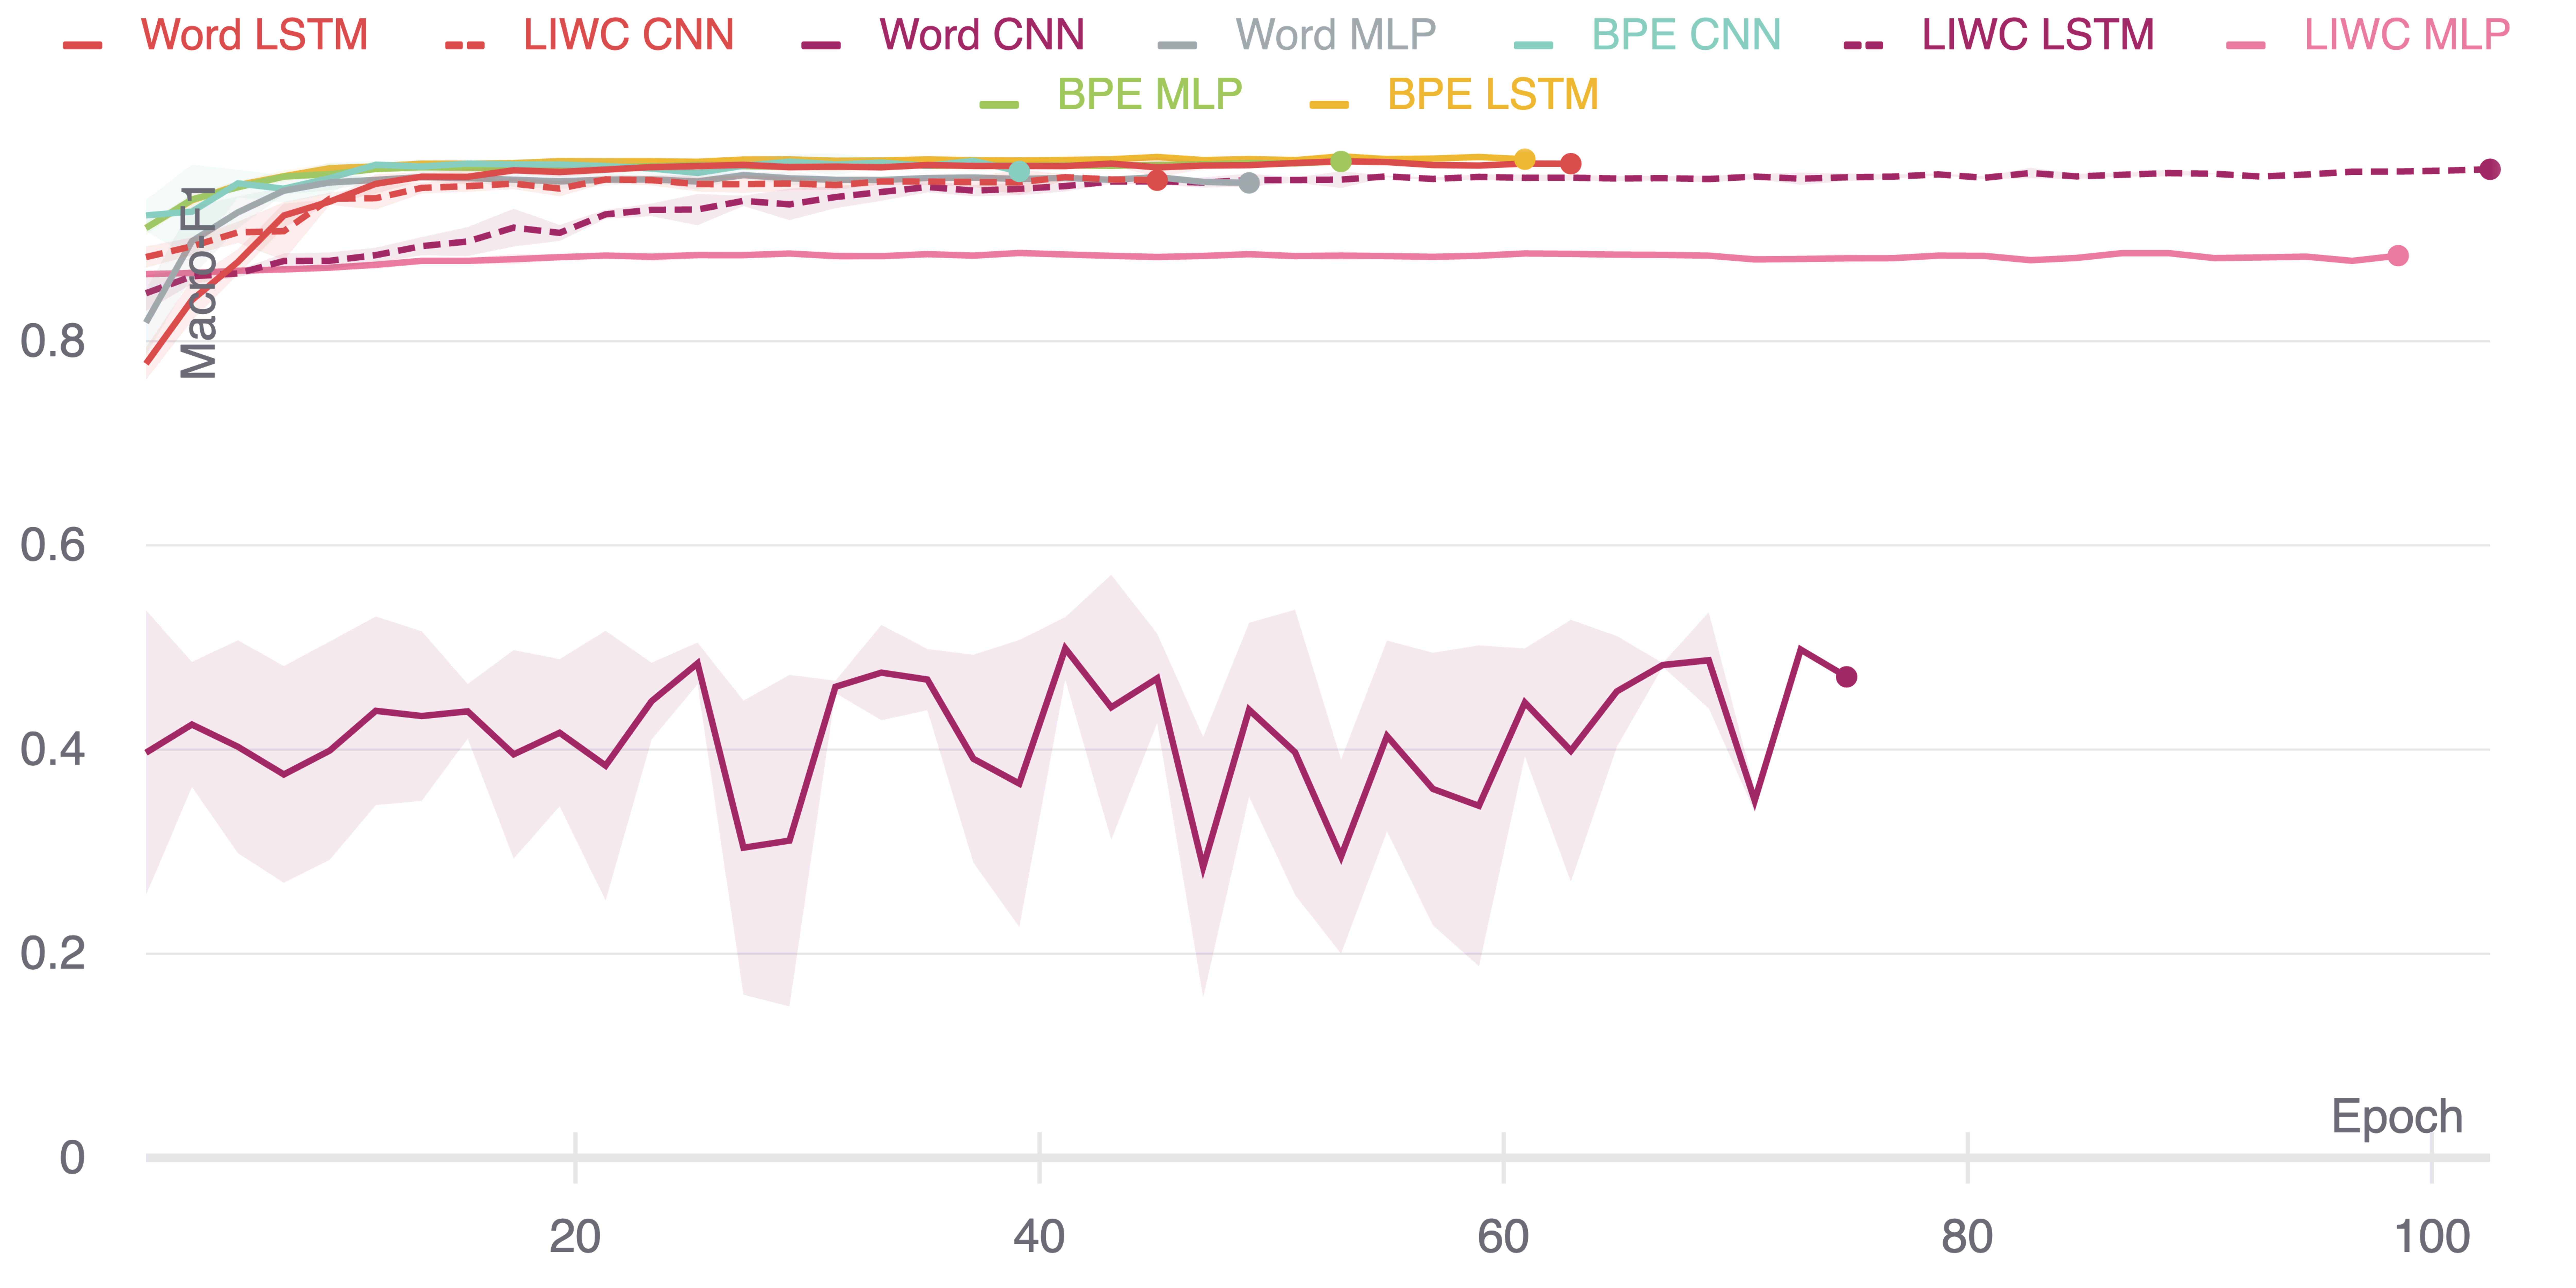
\includegraphics[width=\textwidth]{davidson_dev_f1.pdf}
    \caption{in-domain macro \texttt{f1-score} on validation set for models optimised on the \textit{offence} dataset.}
    \label{fig:davidson_dev_f1}
\end{figure}

\begin{figure}
    \centering
    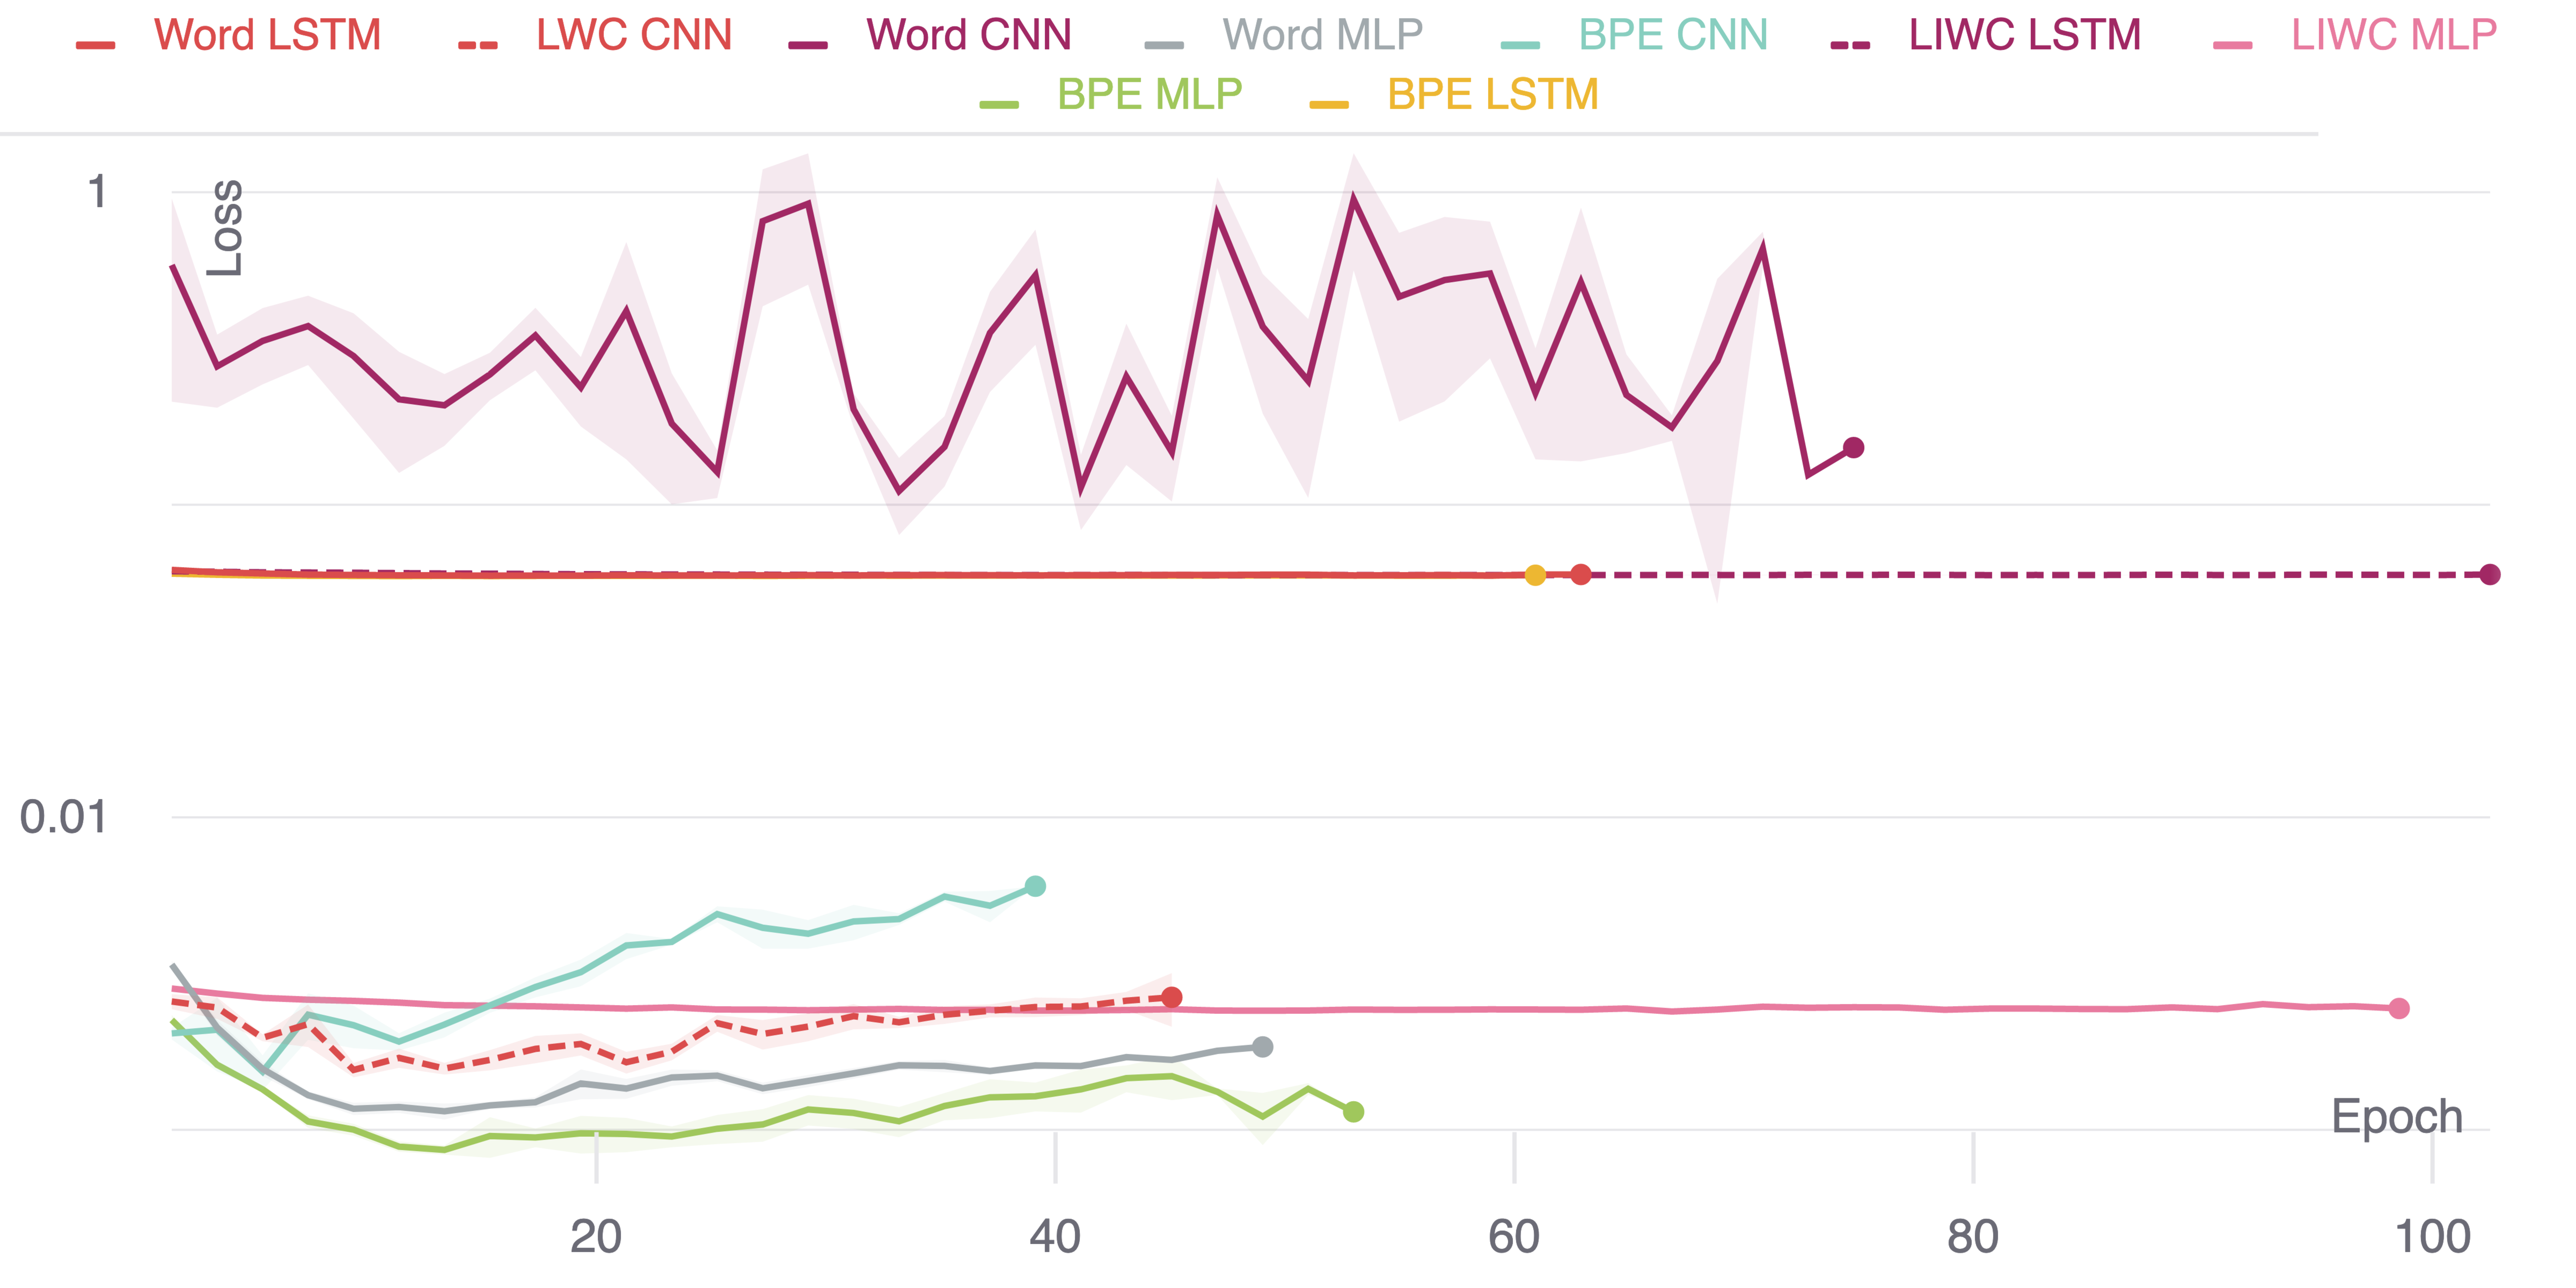
\includegraphics[width=\textwidth]{davidson_dev_loss_stderr_logscale.pdf}
    \caption{validation losses for models optimised on the \textit{offence} dataset.}
    \label{fig:davidson_dev_loss}
\end{figure}

in observing the \texttt{f1-score}s on the validation sets in \cref{fig:davidson_dev_f1,fig:wulczyn_dev_f1,fig:waseem_dev_f1,fig:waseem_hovy_dev_f1,fig:garcia_dev_f1}, a general pattern emerges in which most models, regardless of input type, display similar learning curves.
there are however some notable exceptions to this rule.
one such exception can be observed in \cref{fig:davidson_dev_f1}, where the liwc-based cnn displays volatile performances throughout the entire optimisation procedure.
another exception can be observed in \cref{fig:waseem_dev_f1}, where the bpe based mlp model starts with a low performance, but increasingly improves until the final few epochs, where the model predictions become very volatile and ultimately triggers early stopping with a large drop in performance.
in addition to these two exceptions, the models that are optimised for the \textit{stormfront} dataset (see \cref{fig:garcia_dev_f1})  in which three patterns emerge: first, there are some models that show a large variability in their performances from epoch to epoch, these models tend to trigger early stopping at an early stage; second, there are models that show a smaller degree of variability in classification performance as the model is optimised, but as they pass through the epochs, the model performance steadily increases and the variability in performances decreases; and third, there are models that obtain a high score early in the optimisation procedure and trigger early stopping at an early stage.

another exception can be observed in the models optimised on \textit{toxicity} dataset (see \cref{fig:wulczyn_dev_f1}).
here three salient trends occur.
in the first, models start with a high \texttt{f1-score} and show little improvement as over the epochs and trigger early stopping.
in the second, models start with a lower \texttt{f1-score} and show steady improvements until early stopping is triggered.
the third trend starts with a relatively low model performance (below $0.4$ in \texttt{f1-score}), seeing steady improvements, before reaching a plateau and continuing until early stopping is triggered or the set number of epochs is reached.
as these models are being optimised, there is an early sharp increase in the model performances followed by reaching a plateau and only post minor improvements in the later epochs.

turning to the loss developments in \cref{fig:davidson_dev_loss,fig:wulczyn_dev_loss,fig:waseem_dev_loss,fig:waseem_hovy_dev_loss,fig:garcia_dev_loss} there are three unique patterns: first, the loss rises throughout the optimisation process; second, the loss remains almost entirely unchanged throughout the entire optimisation process, and finally the third pattern; the loss is volatile throughout the process, rising or dropping from epoch to epoch.

\begin{figure}
    \centering
    \includegraphics[width=\textwidth]{wulczyn_dev_f1.pdf}
    \caption{in-domain macro \texttt{f1-score} on validation set for models optimised on the \textit{toxicity} dataset.}
    \label{fig:wulczyn_dev_f1}
\end{figure}
\begin{figure}
    \centering
    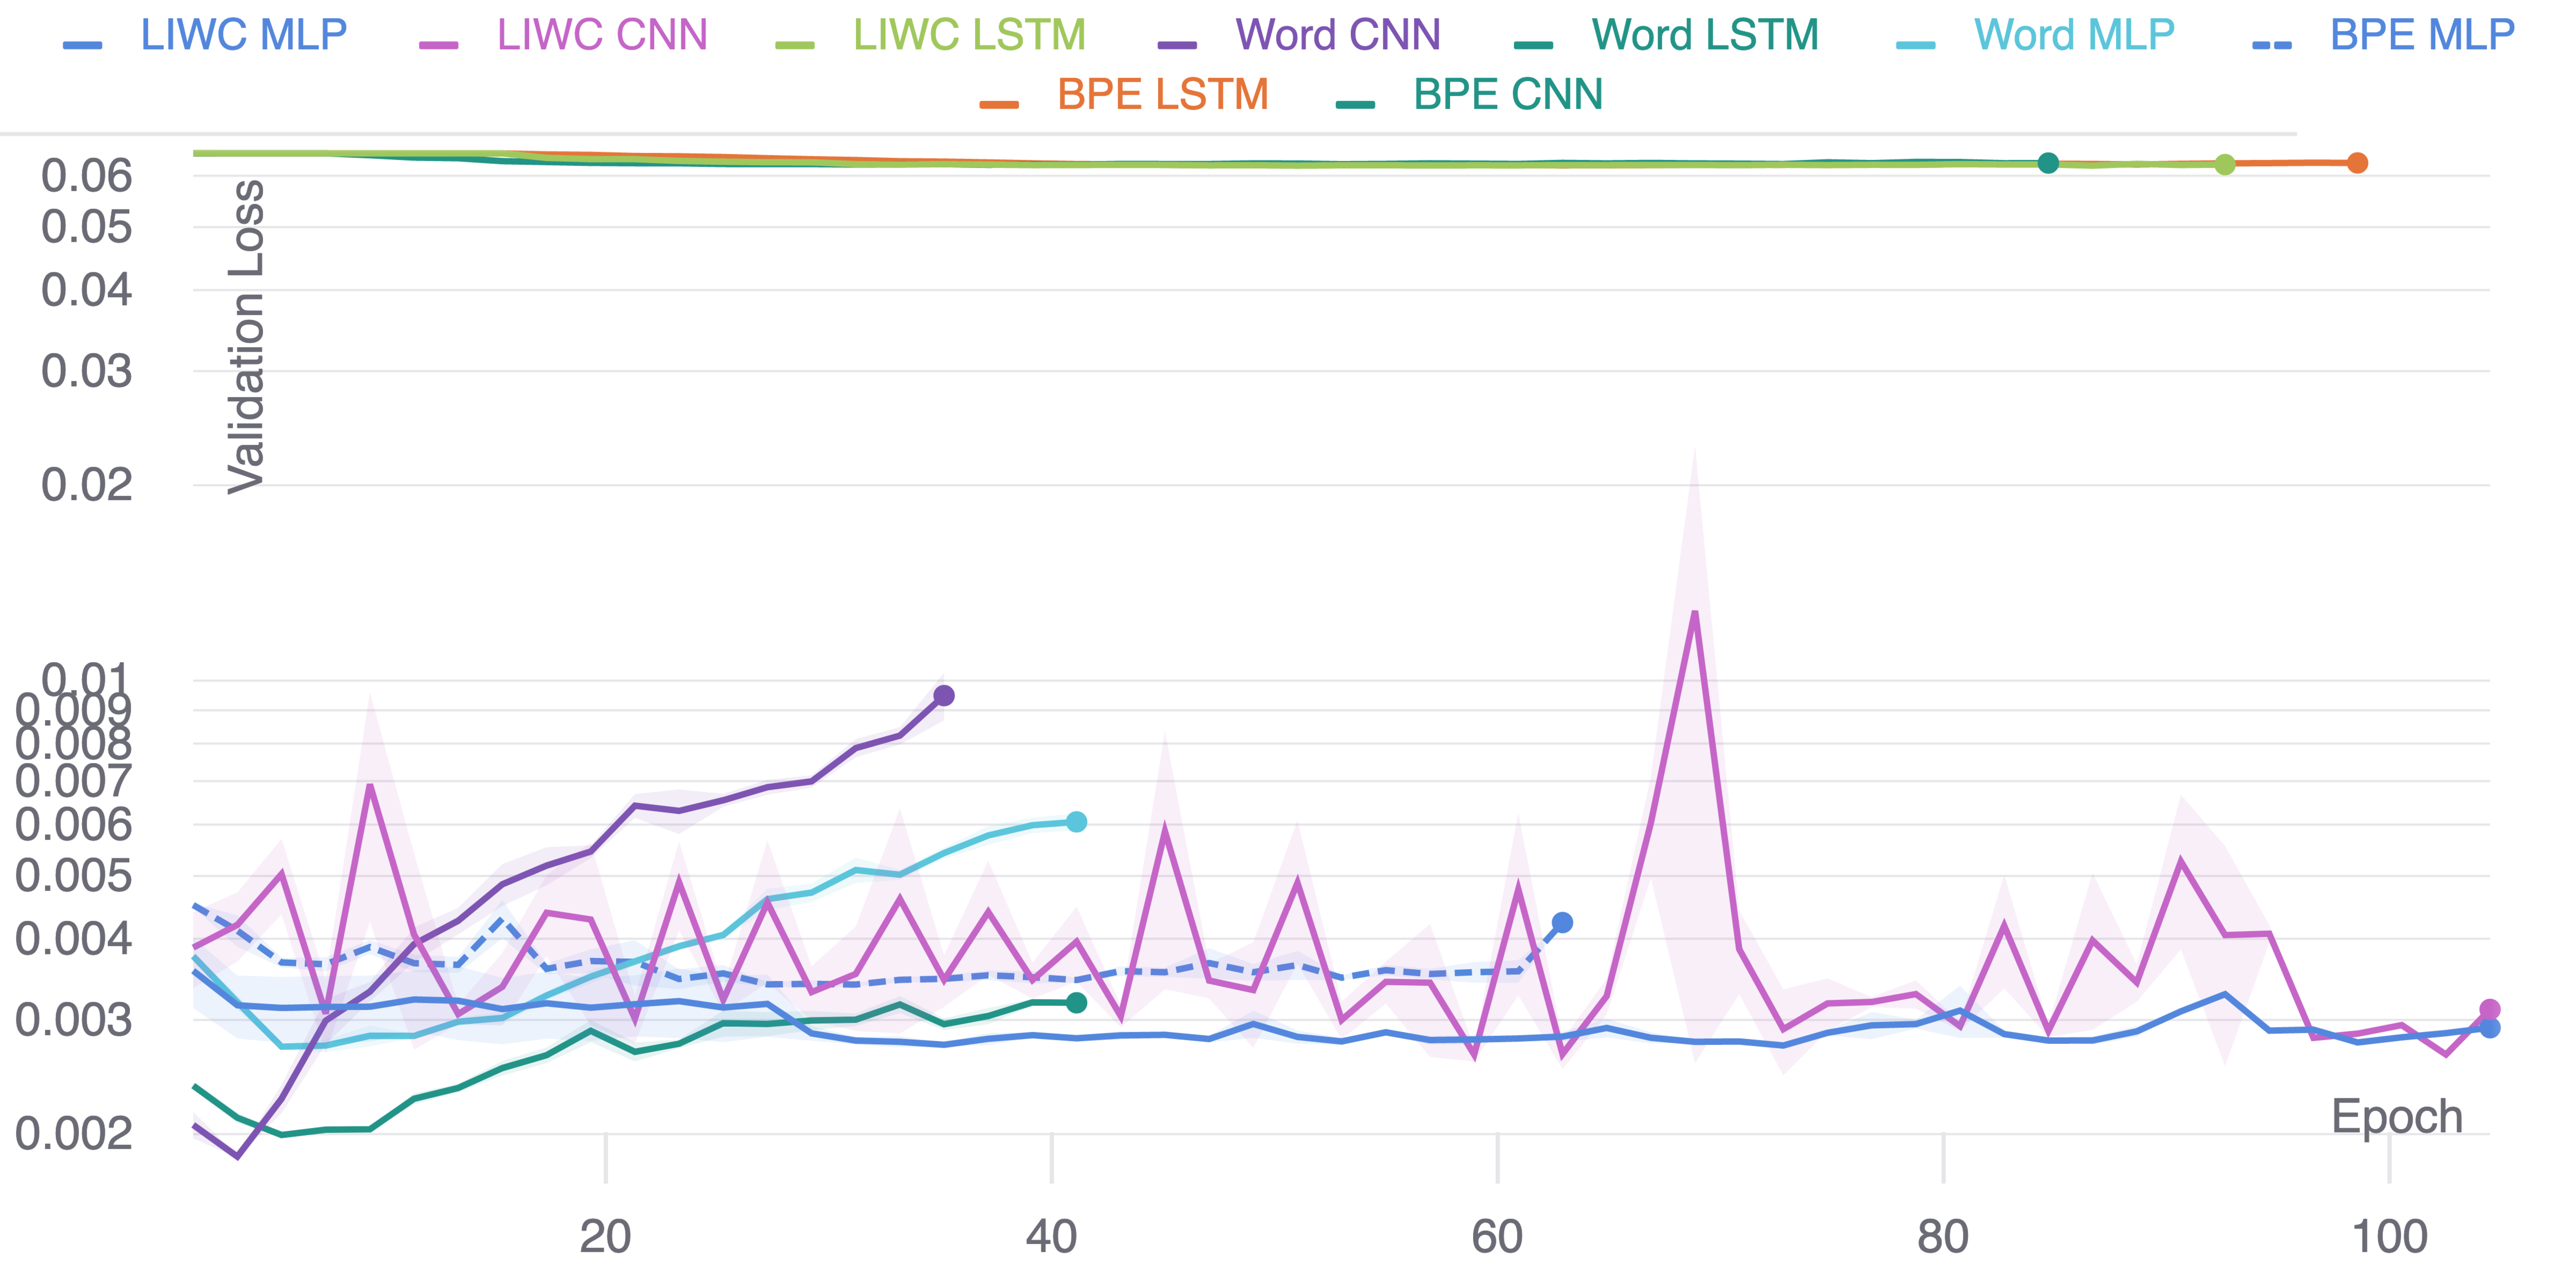
\includegraphics[width=\textwidth]{wulczyn_dev_loss_stderr_logscale.pdf}
    \caption{validation losses for models optimised on the \textit{toxicity} dataset.}
    \label{fig:wulczyn_dev_loss}
\end{figure}

\begin{figure}
    \centering
    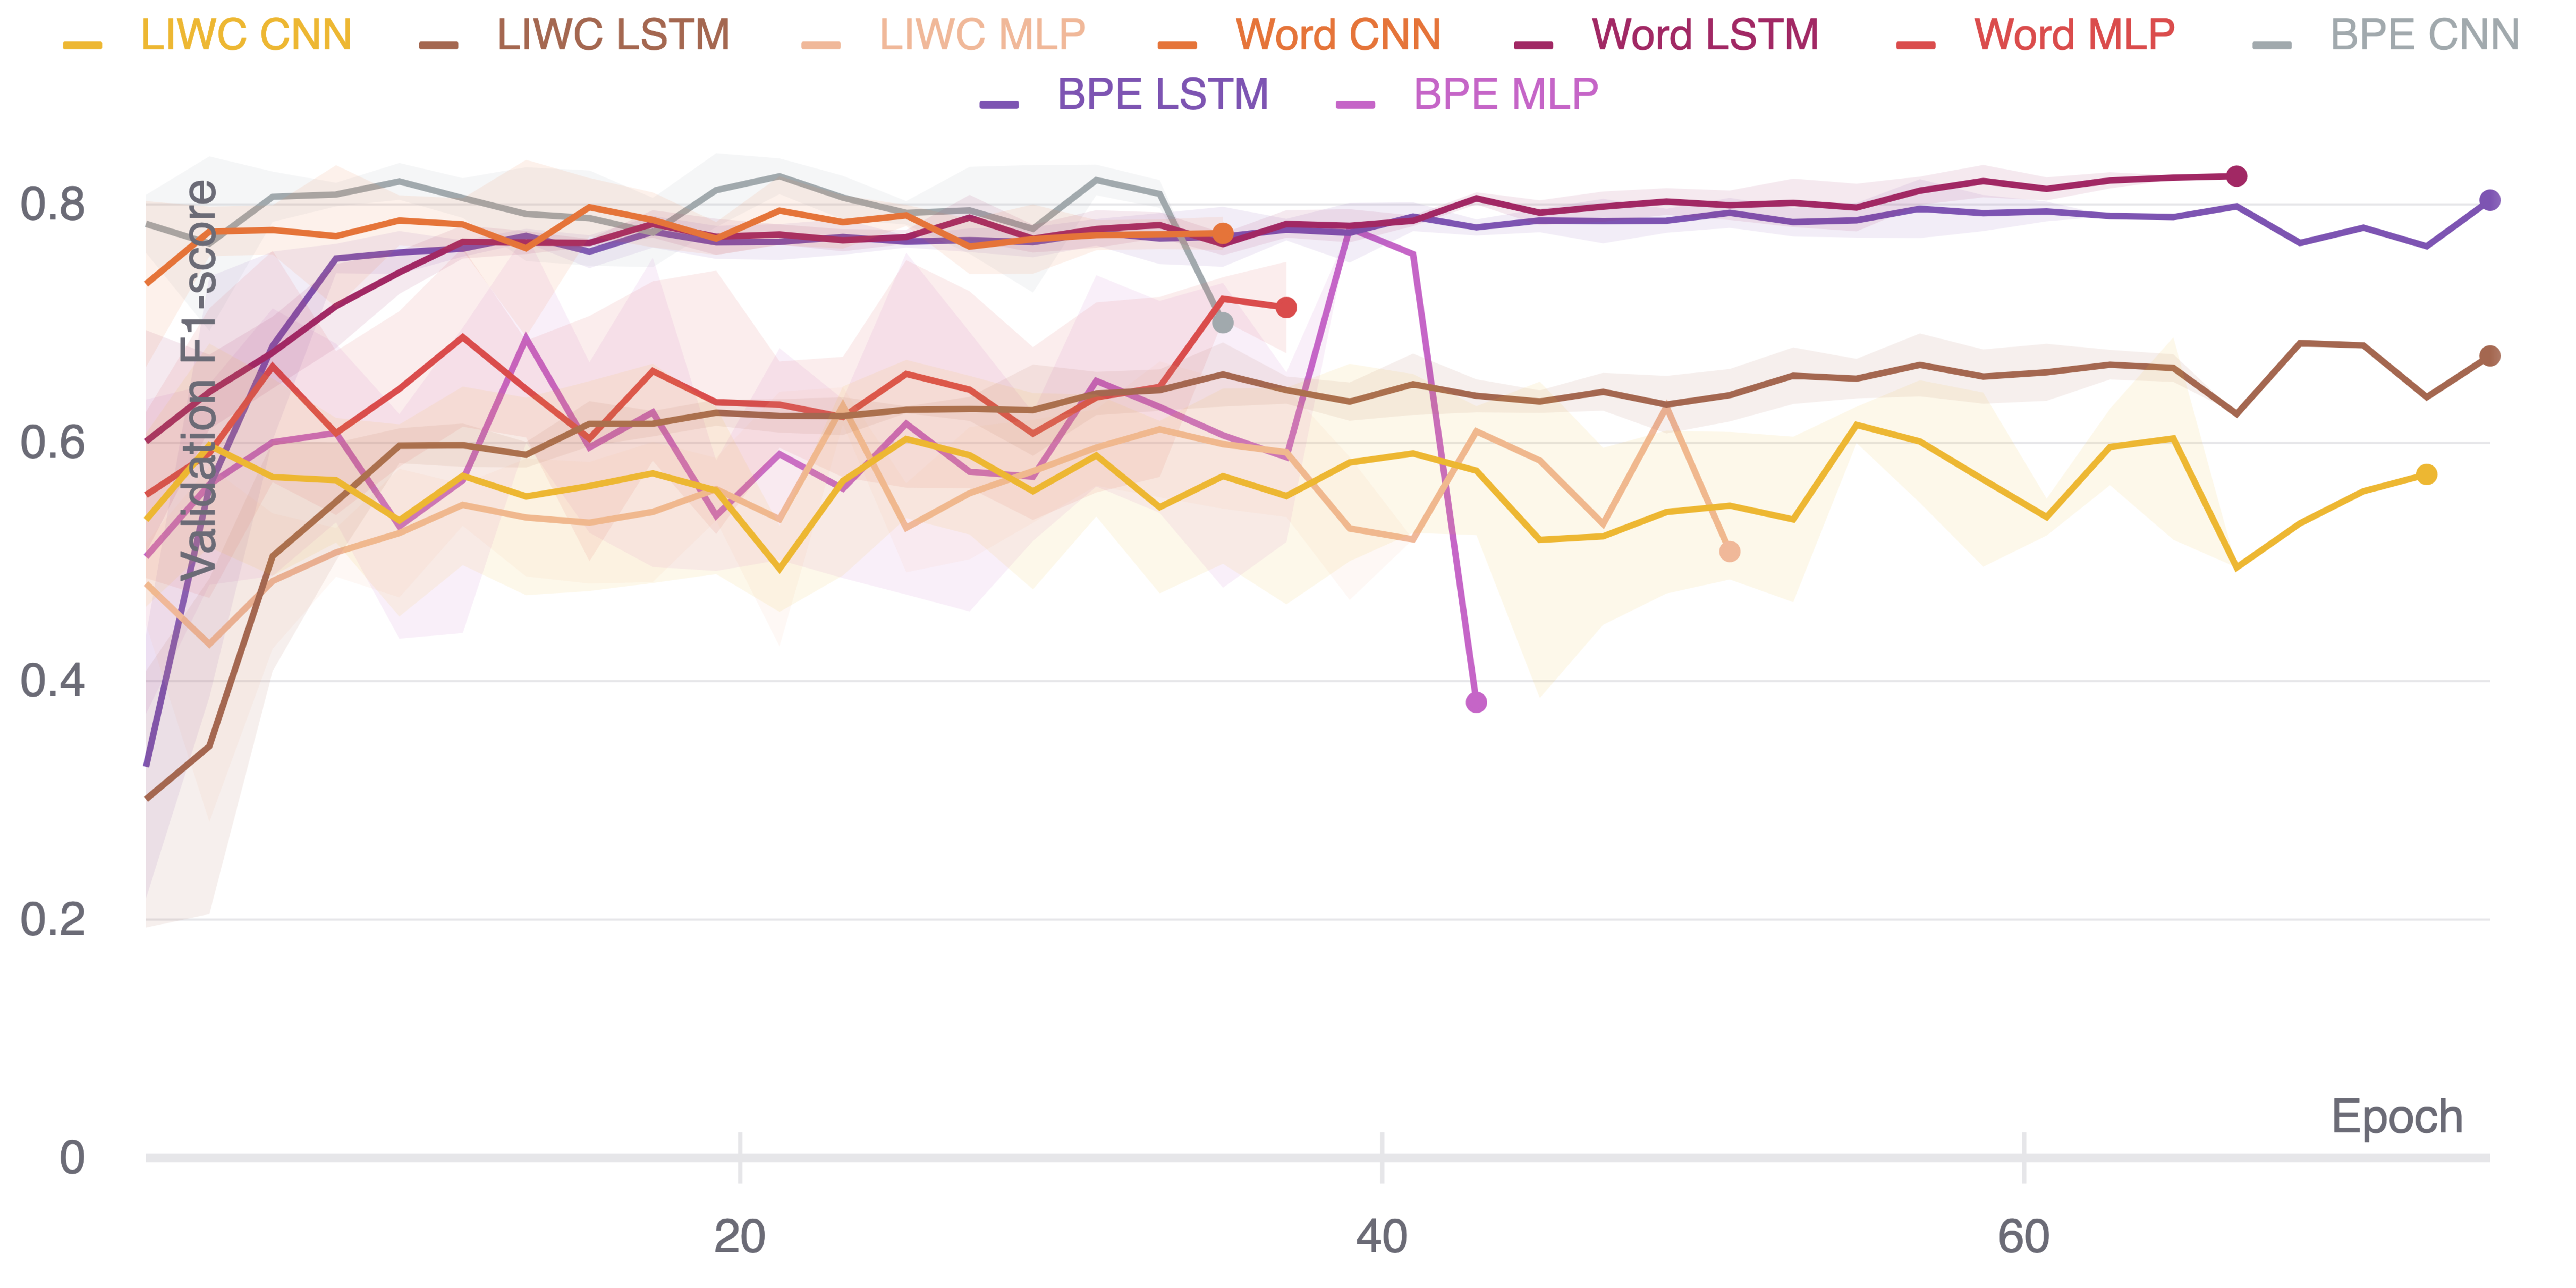
\includegraphics[width=\textwidth]{waseem_dev_f1.pdf}
    \caption{in-domain macro \texttt{f1-score} on validation set for models optimised on the \textit{hate expert} dataset.}
    \label{fig:waseem_dev_f1}
\end{figure}
\begin{figure}
    \centering
    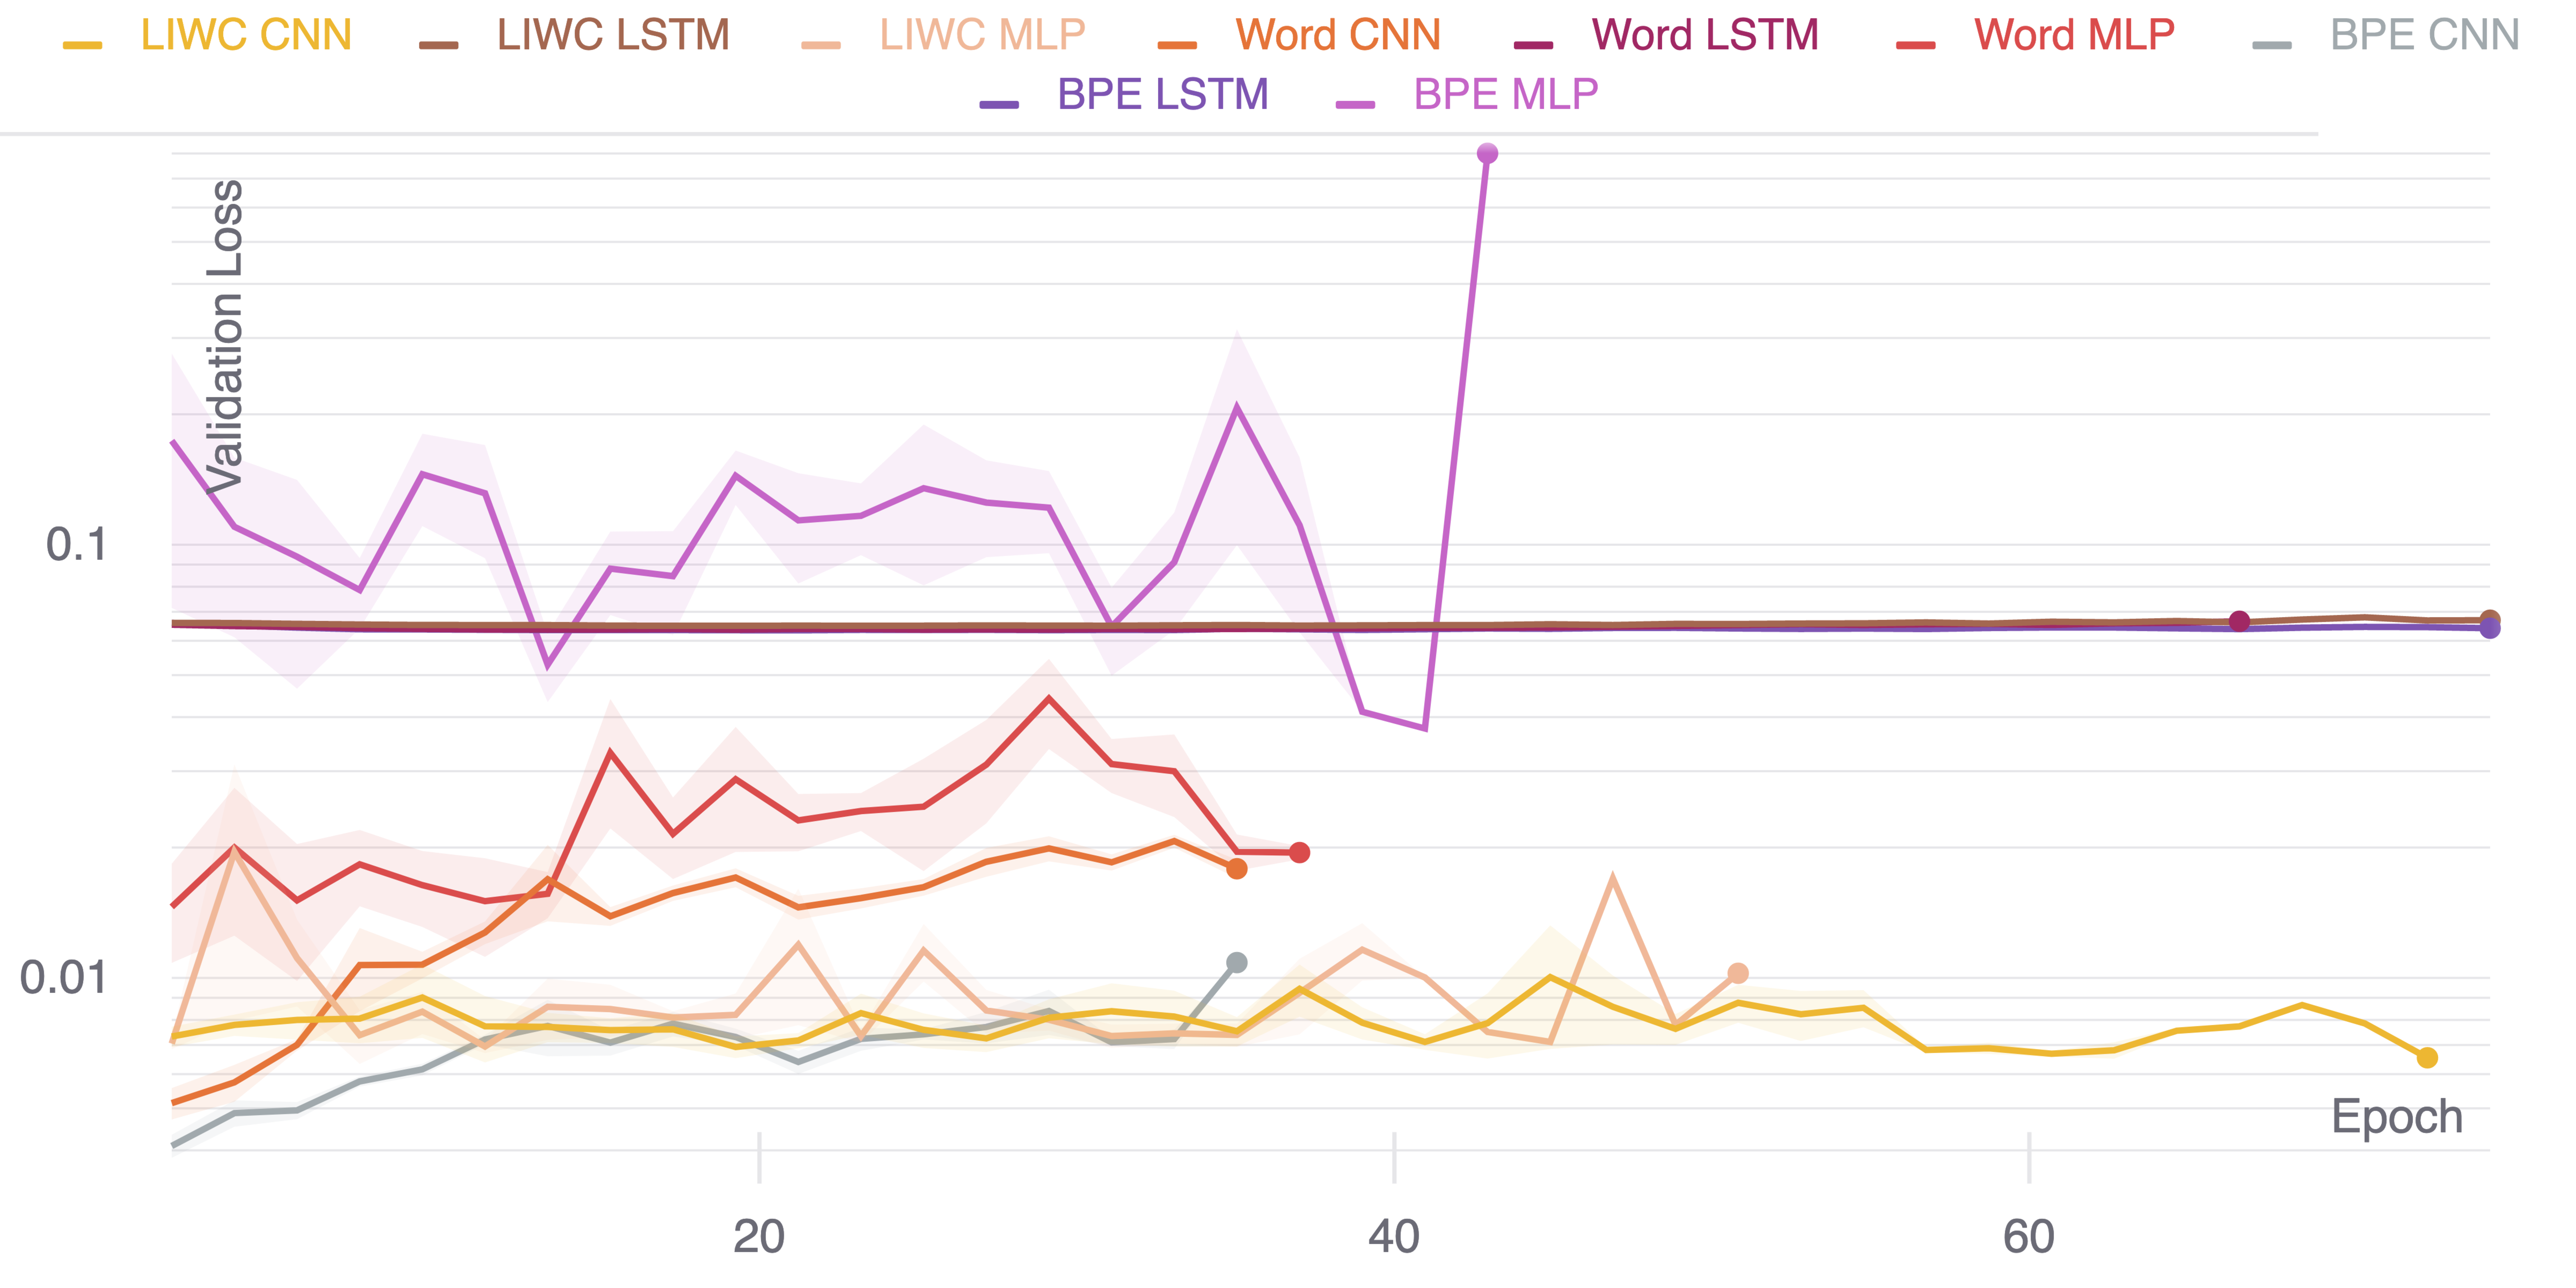
\includegraphics[width=\textwidth]{waseem_dev_loss_stderr_logscale.pdf}
    \caption{validation losses for models optimised on the \textit{hate expert} dataset.}
    \label{fig:waseem_dev_loss}
\end{figure}

\begin{figure}
    \centering
    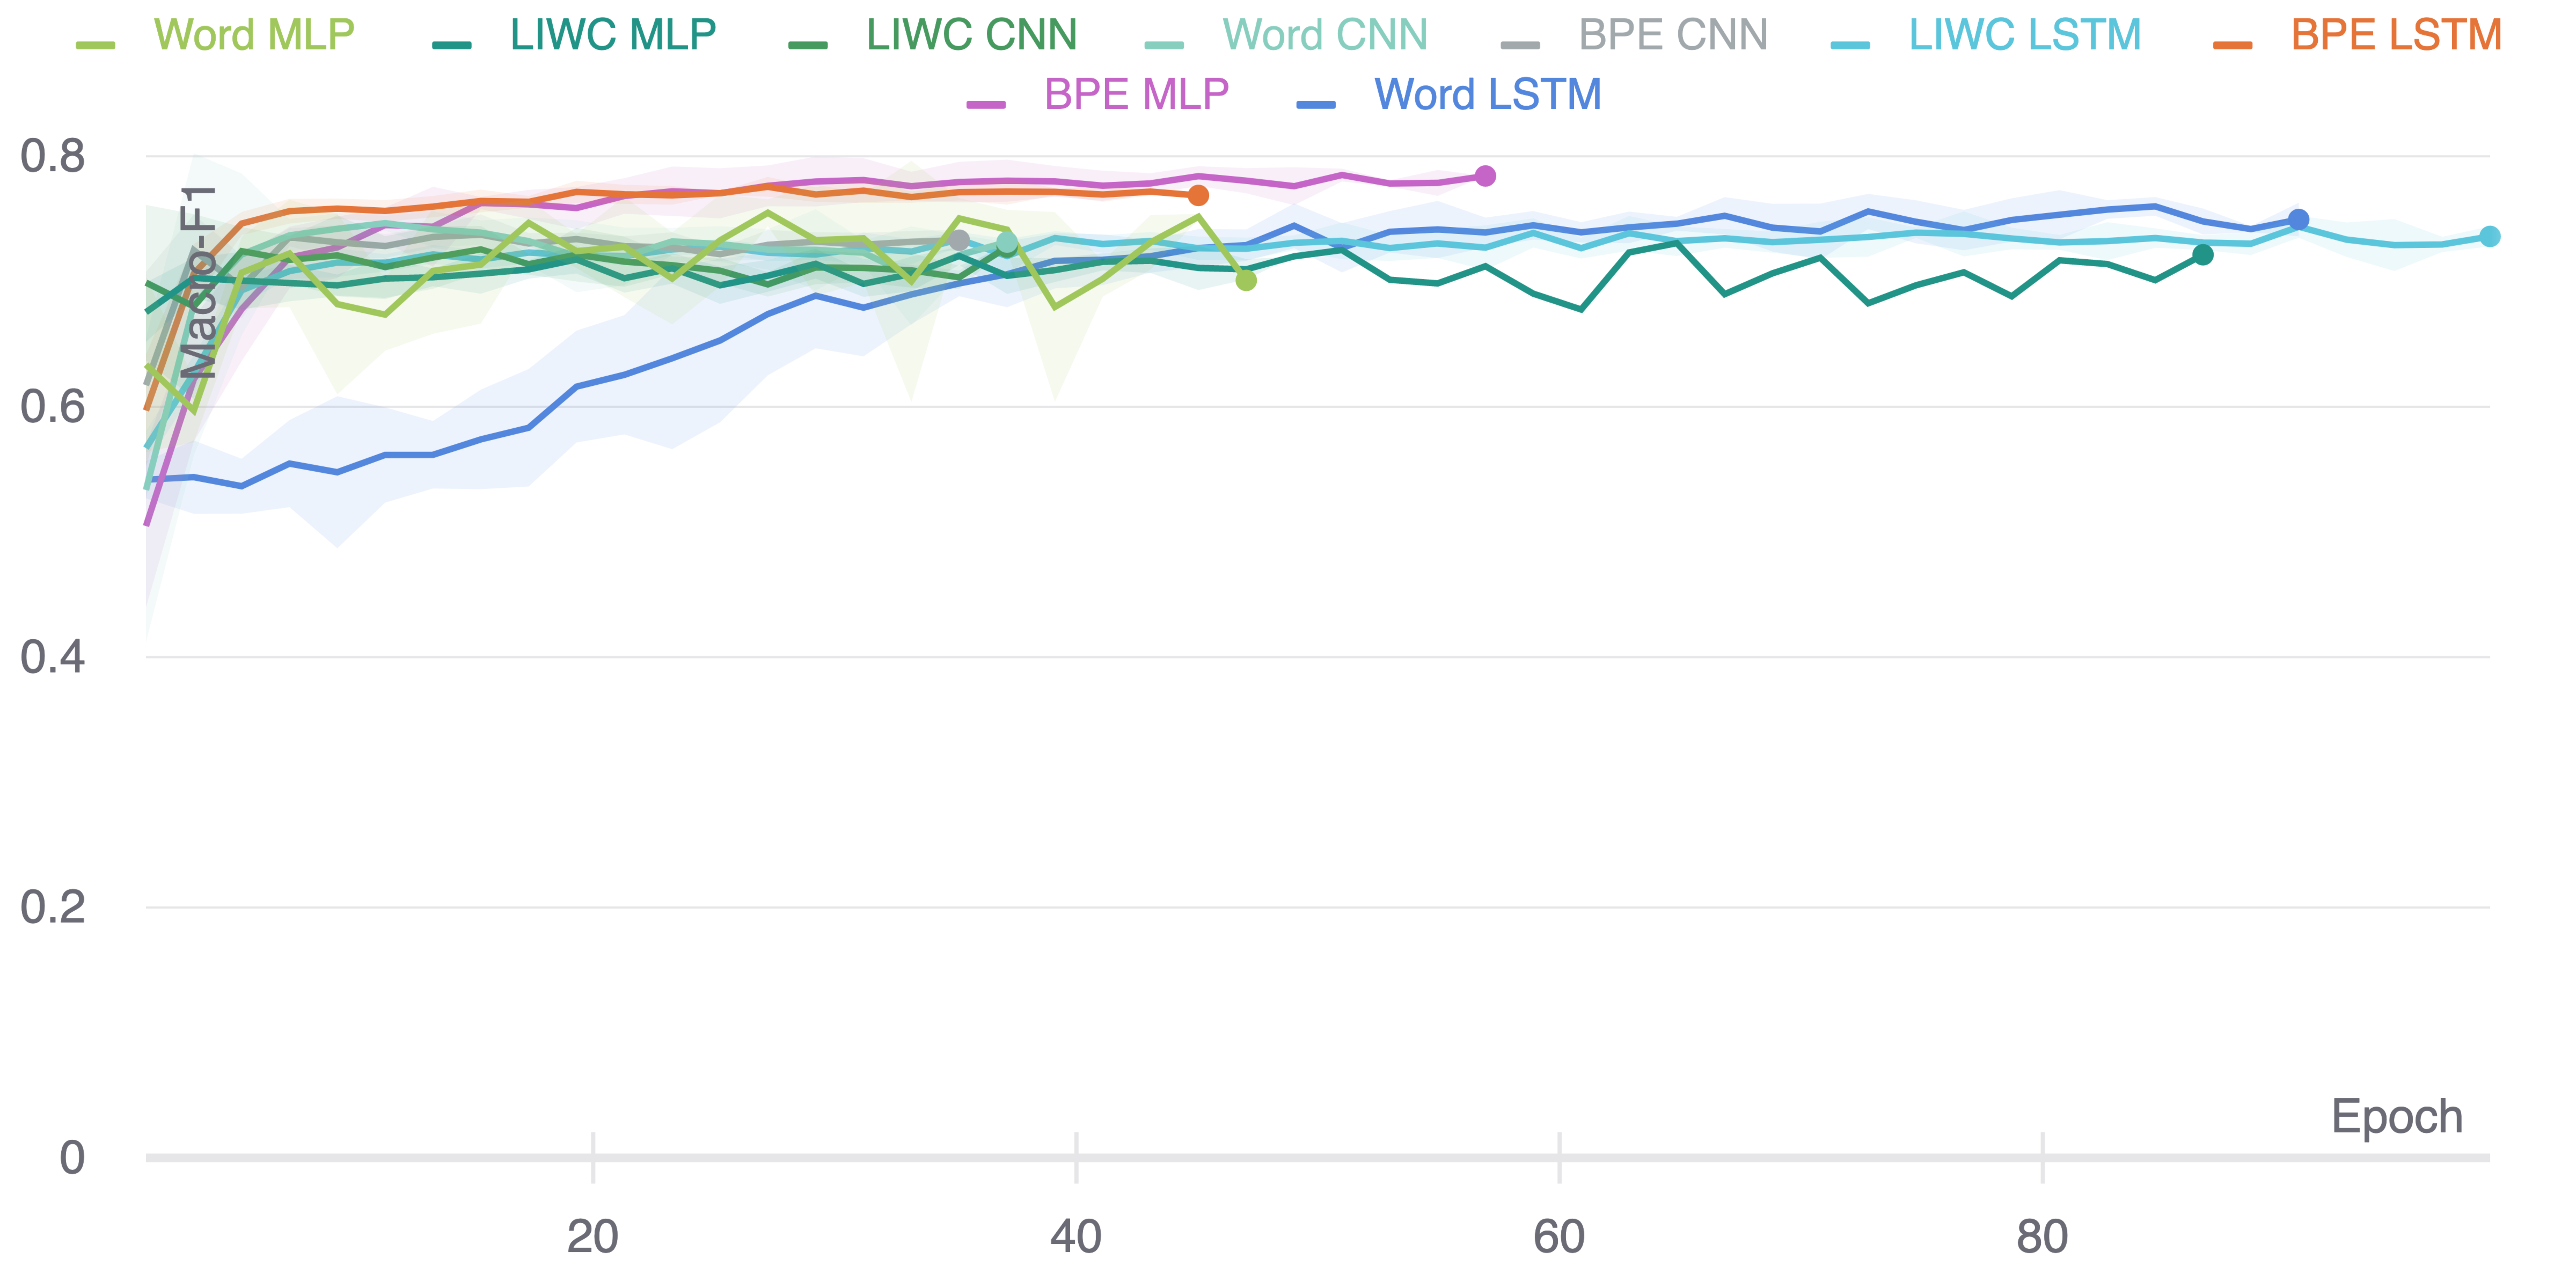
\includegraphics[width=\textwidth]{waseem_hovy_dev_f1.pdf}
    \caption{in-domain macro \texttt{f1-score} on validation set for models optimised on the \textit{hate speech} dataset.}
    \label{fig:waseem_hovy_dev_f1}
\end{figure}
\begin{figure}
    \centering
    \includegraphics[width=\textwidth]{waseem_hovy_dev_loss_stderr_logscale.pdf}
    \caption{validation losses for models optimised on the \textit{hate speech} dataset.}
    \label{fig:waseem_hovy_dev_loss}
\end{figure}

\begin{figure}
    \centering
    \includegraphics[width=\textwidth]{garcia_dev_f1.pdf}
    \caption{in-domain macro \texttt{f1-score} on validation set for models optimised on the \textit{stormfront} dataset.}
    \label{fig:garcia_dev_f1}
\end{figure}
\begin{figure}
    \centering
    \includegraphics[width=\textwidth]{garcia_dev_loss_stderr_logscale.pdf}
    \caption{validation losses for models optimised on the \textit{stormfront} dataset.}
    \label{fig:garcia_dev_loss}
\end{figure}

\subsubsection{evaluation set performances}
in \cref{fig:davidson_mlp_test,fig:wulczyn_mlp_test,fig:waseem_mlp_test,fig:waseem_mlp_test,fig:garcia_mlp_test,fig:davidson_lstm_test,fig:wulczyn_lstm_test,fig:waseem_lstm_test,fig:waseem_lstm_test,fig:garcia_lstm_test,fig:davidson_cnn_test,fig:wulczyn_cnn_test,fig:waseem_cnn_test,fig:waseem_cnn_test,fig:garcia_cnn_test}, i show the in-domain and out-of-domain results of using the neural network architectures described in \cref{sec:liwc_modelling} for modelling abuse using the three different document representations.
the bars in each figure represent the scores of each models on the test set in question, e.g. in \cref{fig:davidson_mlp_test} i show the macro \texttt{f1-score}s achieved by all models on the test set for the \textit{offence} dataset, and the error bars are the standard deviation over the $5$ parameter seed runs.

considering figures collectively, it's clear that in-domain models in most cases, predictably, out-perform models optimised on out-of-domain datasets.
interestingly, it's also clear that liwc-based models in many cases are comparable to models using full surface-form vocabulary.
moreover, this similarity in performance largely also holds for out-of-domain performance, with some liwc based models consistently ranking among the best performing out-of-domain models.
the comparison of out-of-domain performance between experimental models and the linear baselines too is worth noting.
here, in spite of improved performances on the in-domain evaluation sets, there is a tend towards a slight decrease performance on out-of-domain data by the experimental models.

one dataset however, is notable in its in-domain and all out-of-domain predictions: the \textit{stormfront} dataset. 
for this dataset, linear models perform at par, or better than all configurations of neural models.
the most likely explanation for this can be found in the small dataset size of less than $3,000$ documents.
one way to address such a short-coming of this dataset is to increase the dataset size. 
although the experiments i conduct with the dataset keep the number of documents lower than the total annotated set in order to maintain a balanced dataset, the dataset does in some cases out-perform models that are optimised on larger dataset for out-of-domain prediction, i.e. in the mlp models evaluated on the \textit{offence} data (see \cref{fig:davidson_mlp_test}, where the stormfront liwc based model  out-performs several other models that are optimised on larger datasets.
%specifically, models trained on the \textit{stormfront} dataset have comparable out-of-domain classification performance with the \textit{offence} dataset on the evaluation sets for the \textit{hate expert} dataset (see \cref{fig:waseem_mlp_test,fig:waseem_lstm_test,fig:waseem_cnn_test,fig:waseem_hovy_mlp_test,fig:waseem_hovy_lstm_test,fig:waseem_hovy_cnn_test}).

more generally, from the out-of-domain classification performances, there seems to be a correlation with the goals of the datasets and out-of-domain performance.
for instance, in \cref{fig:davidson_mlp_test,fig:davidson_lstm_test,fig:davidson_cnn_test,fig:wulczyn_mlp_test,fig:wulczyn_cnn_test}, i observe that models optimised on the \textit{offence} and \textit{toxicity} datasets out-perform models optimised on other datasets.
for both of these datasets, the governing understanding of abuse and hate speech are that not all speech that is offensive is necessarily also problematic.
the motivation for the development of the \textit{offence} dataset was specifically to disentangle hateful from offensive.
similarly, the \textit{toxicity} dataset asked its annotators to identify comments that might make people exit conversations they were part of rather than ask annotators to label for all content that is offensive or hateful.
thus, for these two datasets, the governing question is not necessarily the protection of marginalised communities and identities but instead identifying a degree of acceptable abuse and hostility.

in contrast, the \textit{hate expert} and \textit{hate speech} datasets seek to identify communications that are harmful to marginalised communities.
thus, it's no surprise that the out-of-domain performances for models optimised on these two datasets perform reasonably well with each other.
however here it is also clear that there is an influence of dataset size. 
where the \textit{hate speech} dataset consists of $~16,000$ documents, the \textit{hate expert} dataset consists of $~7,000$ documents, which is also apparent from the fact that the models optimised on the \textit{hate speech} dataset perform better on the \textit{hate expert} evaluation set than the models optimised on the \textit{hate expert} dataset perform on the \textit{hate speech} dataset.

the \textit{stormfront} dataset on the other hand is annotated to identify deliberate attacks against ``specific group[s] of people'' on the basis of their group membership or characteristics of group's identities \citep{garcia:2019}.
this annotation criteria forms a subset of the annotation guidelines that are used for the \textit{hate speech} and \textit{hate expert} datasets.
moreover, the collection strategies for the three datasets also share common characteristics.
where \citet{garcia:2019} specifically seek out content from a white supremacist forum for their dataset, \citet{waseem:2016,waseem-hovy:2016} sample from twitter by searching for keywords that were likely to result in a large set of abuse. 
thus, while the domain of the data and the annotation guidelines are not the same, there are likely to be similarities in the content and annotations produced.

\begin{figure}
\begin{minipage}{\textwidth}
    \centering
    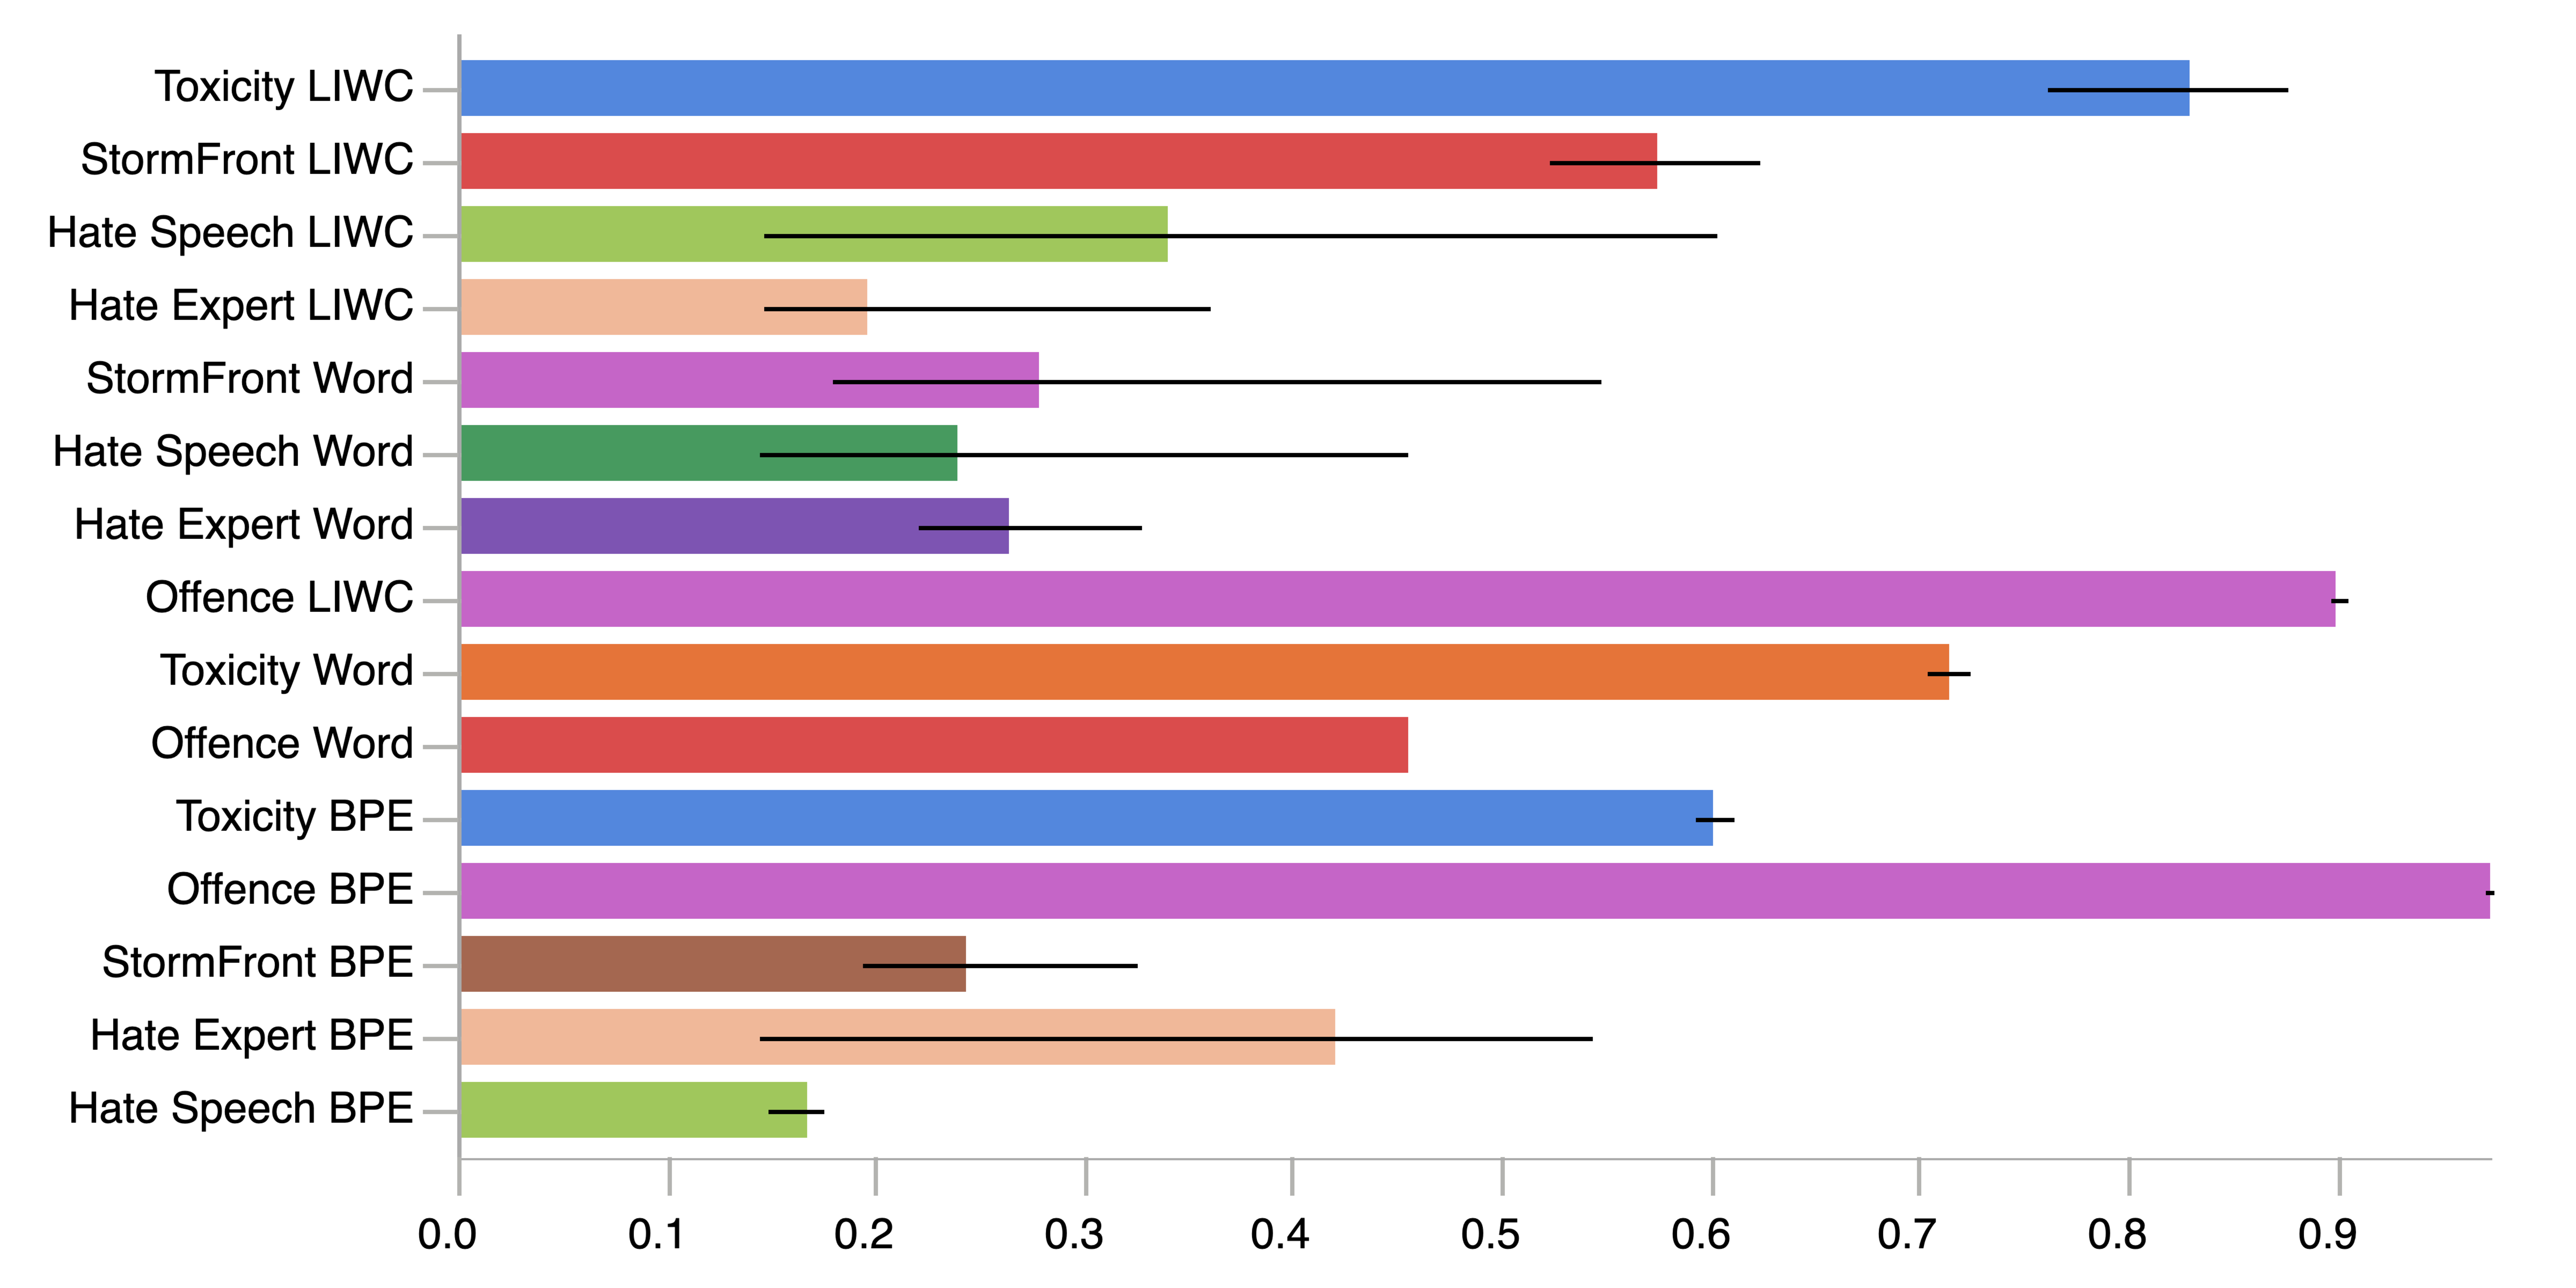
\includegraphics[width=\textwidth]{all_mlp_davidson_test.pdf}
    \caption{macro \texttt{f1-scores} for all mlp models on the \textit{offence} evaluation set with the standard deviation represented in error bars.}
    \label{fig:davidson_mlp_test}
  \vfill
    \includegraphics[width=\textwidth]{all_mlp_wulczyn_test.pdf}
    \caption{macro \texttt{f1-scores} for all mlp models on the \textit{toxicity} evaluation set with the standard deviation represented in error bars.}
    \label{fig:wulczyn_mlp_test}
\end{minipage}
\end{figure}

\begin{figure}
\begin{minipage}{\textwidth}
\centering
    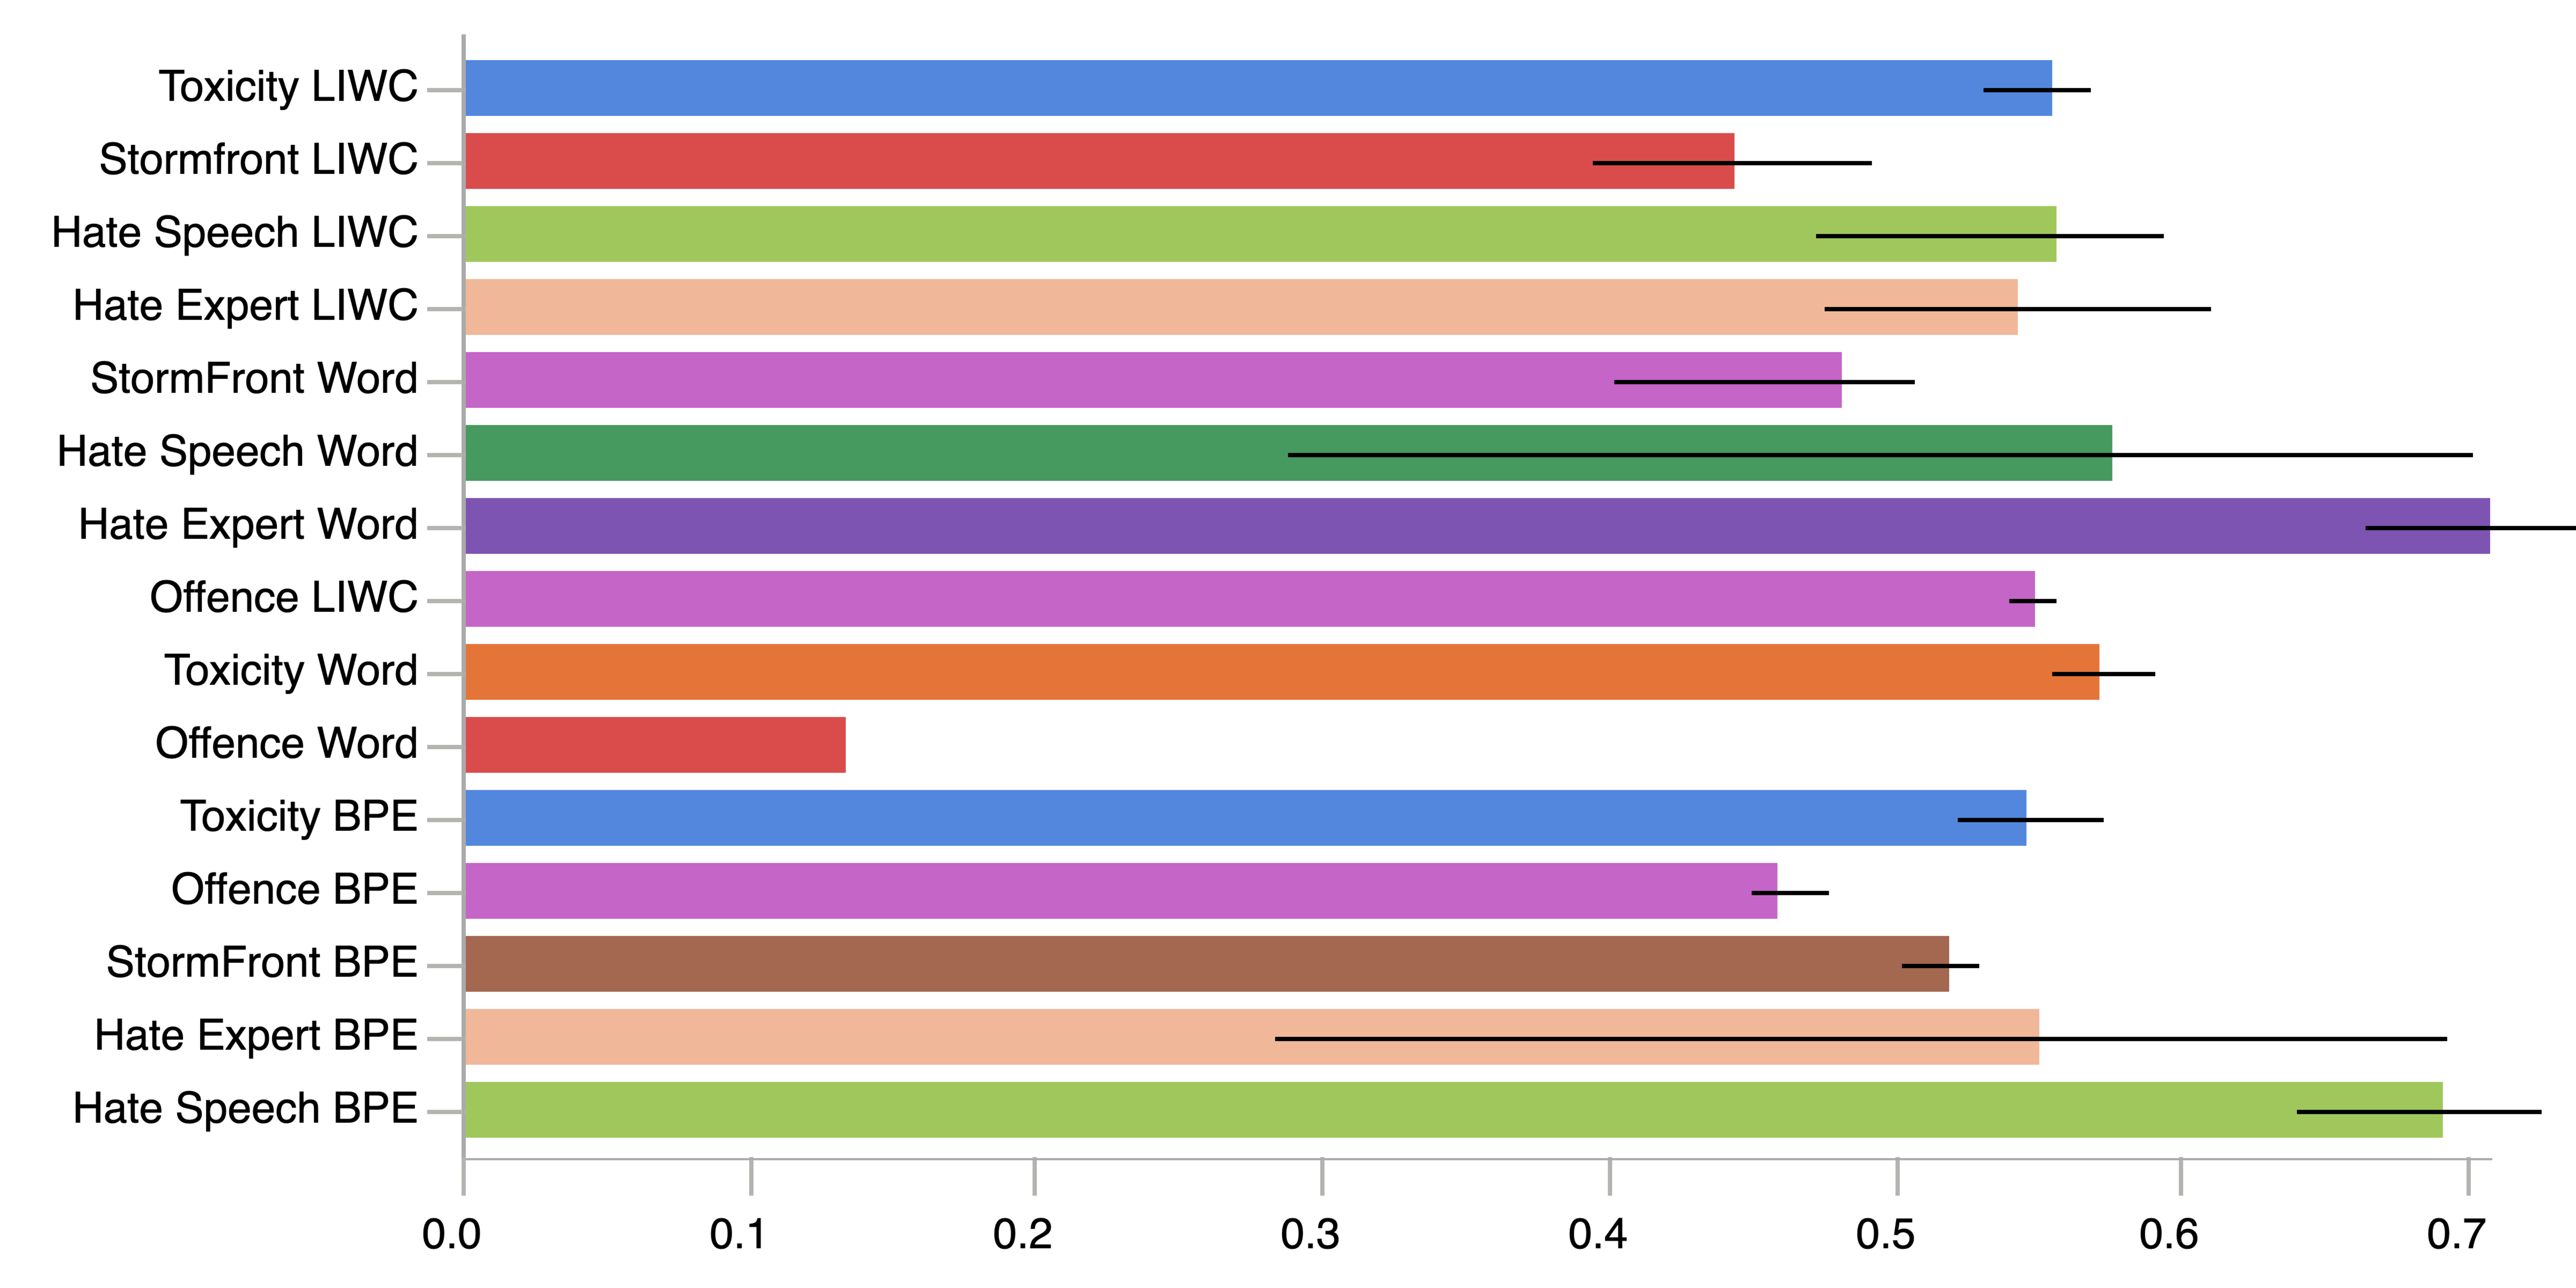
\includegraphics[width=\textwidth]{all_mlp_waseem_test.pdf}
    \caption{macro \texttt{f1-scores} for all mlp models on the \textit{hate expert} evaluation set with the standard deviation represented in error bars.}
    \label{fig:waseem_mlp_test}
    \vfill
      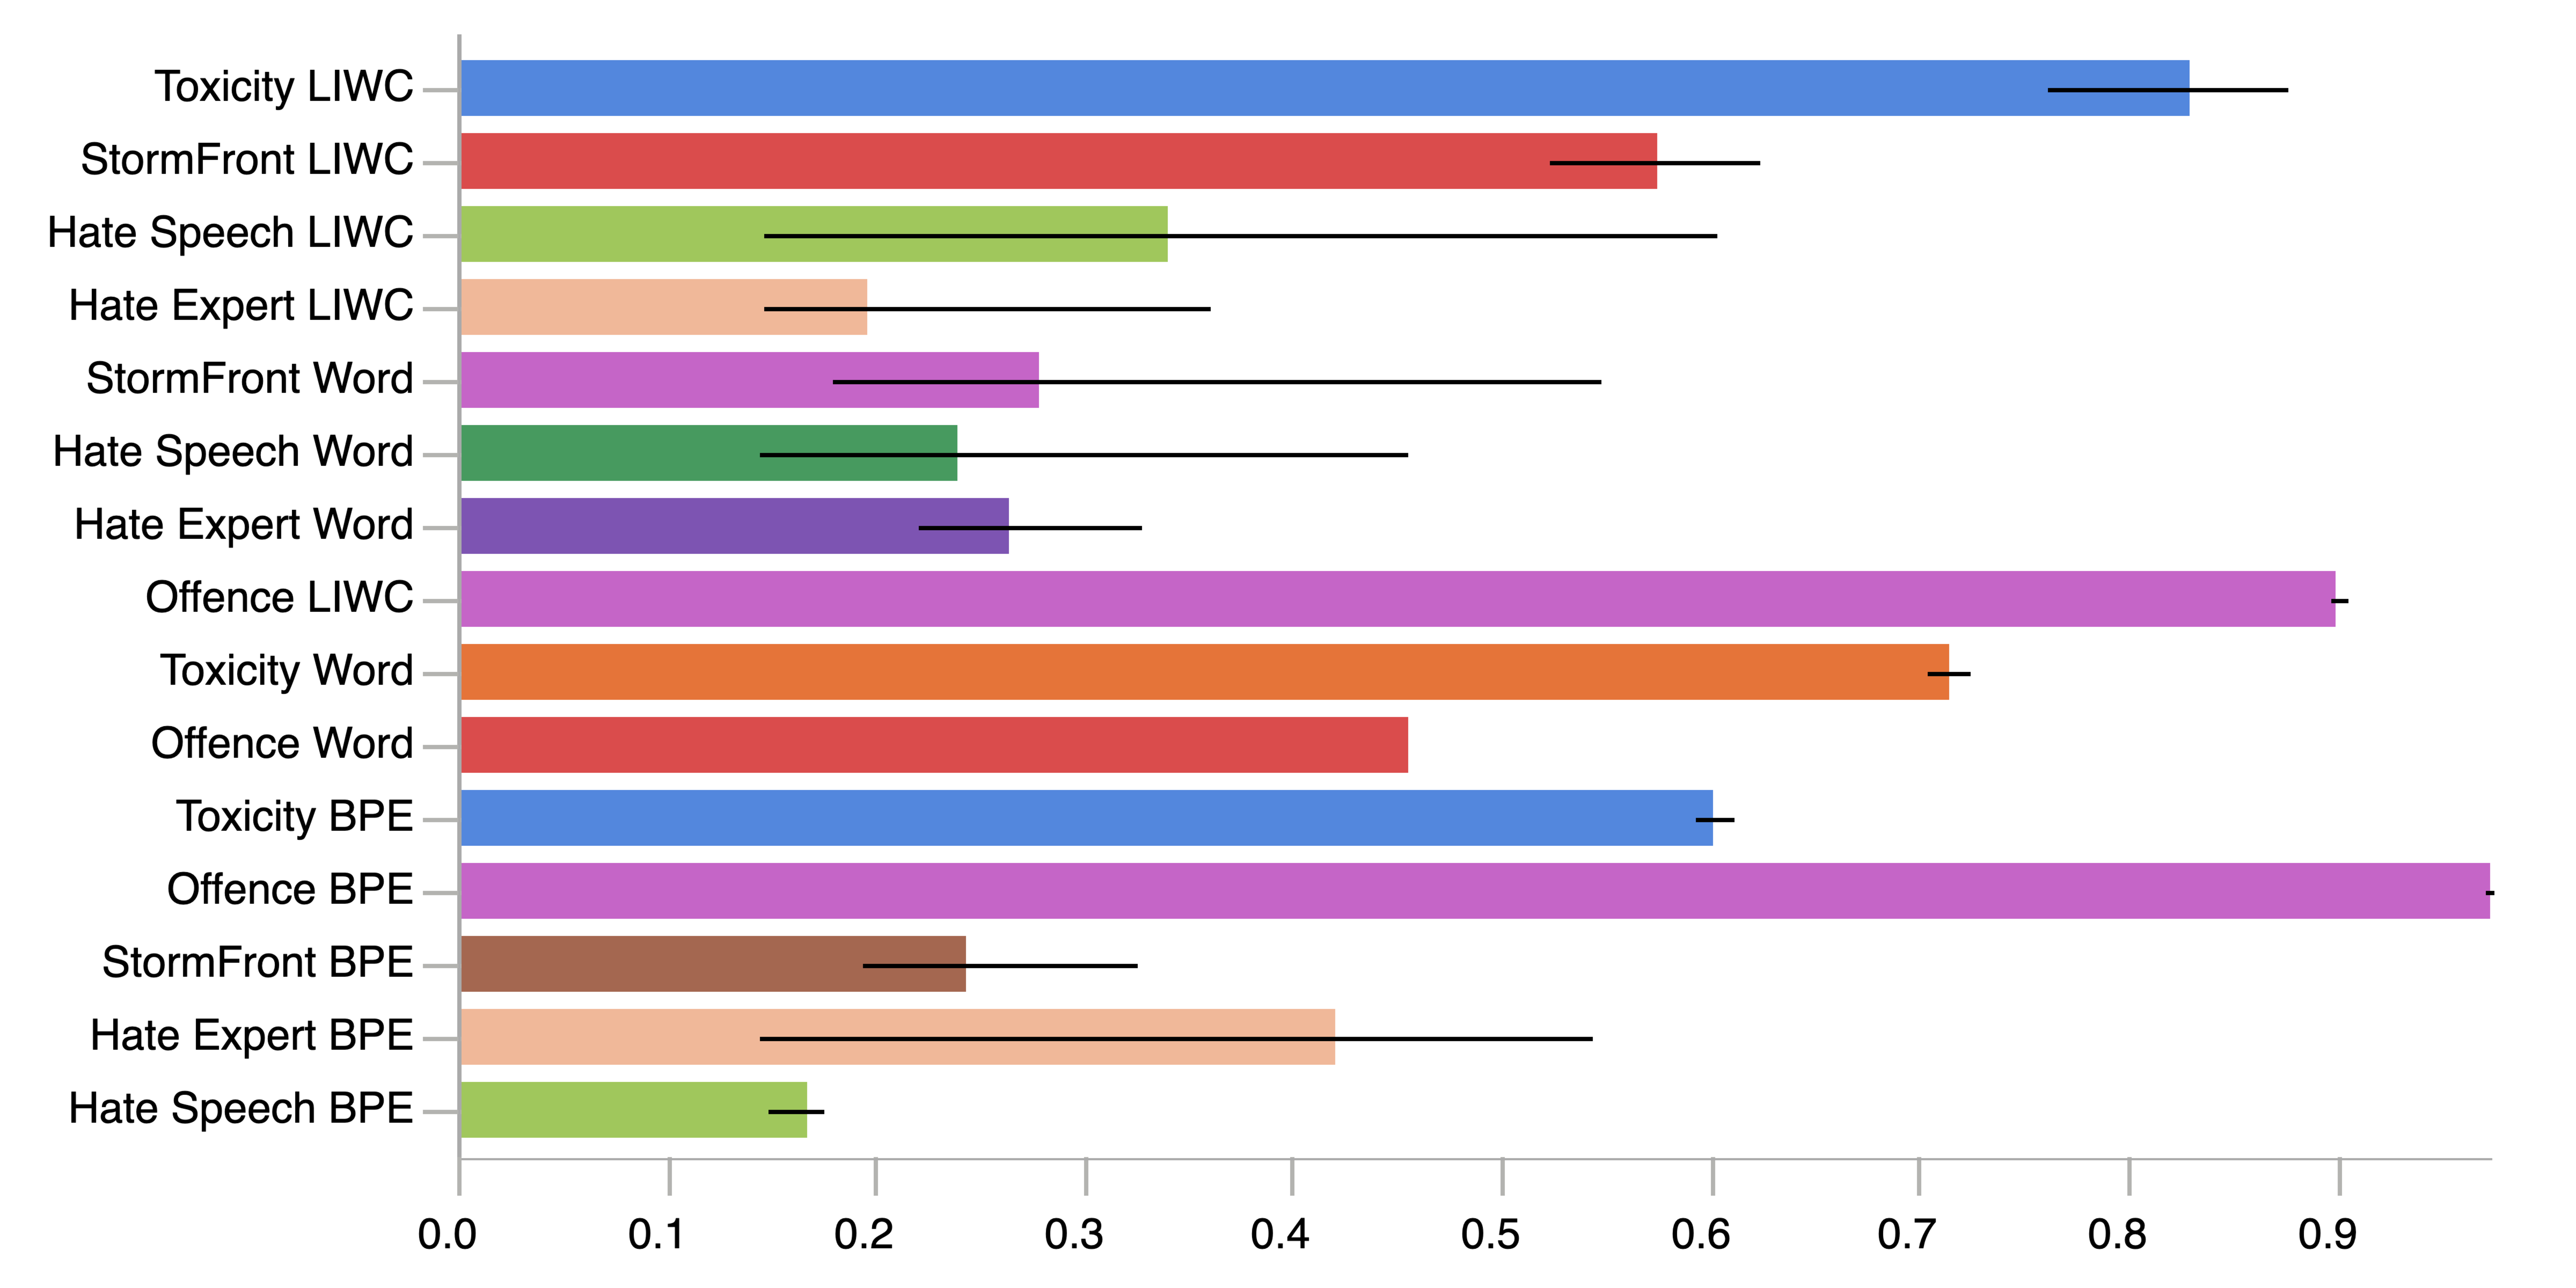
\includegraphics[width=\textwidth]{all_mlp_waseem_hovy_test.pdf}
  \caption{macro \texttt{f1-scores} for all mlp models on the \textit{hate speech} evaluation set with the standard deviation represented in error bars.}
  \label{fig:waseem_hovy_mlp_test}
\end{minipage}
\end{figure}

attending to the questions surrounding the use of liwc to represent documents for modelling abuse, i turn to the baseline and experimental model performances on the validation and evaluation sets of the liwc-based models.
in the validation sets for the linear baselines (see \cref{tab:liwc_baseline_linear_params}), the liwc-based methods do not out-perform any other model type on some datasets while it does on others.
for instance, a highly competitive score is obtained (e.g. $0.9207$ for liwc-based svm model against $0.9222$ for a word-token based svm) .
for other datasets however, the score obtained by liwc-based models is much lower, suggesting that liwc-based modelling may be an appropriate means of modelling abuse under some conditions.
for the neural network based models a similar story presents itself, although the liwc-based models perform reasonably well in comparison to models that use a larger vocabulary (e.g. $0.9644$ for the liwc-based model in \cref{tab:redux_embedding_offence_params} and $0.9783$ for the bpe-based model).

on the evaluation sets however, a slightly different patterns plays out. 
for most evaluation datasets, at least one of the liwc-based models out-perform some of the surface token based models, and in some cases out-perform all other models.
in particular, \cref{fig:wulczyn_mlp_test}, the in-domain liwc-based model out-performs all other model types, though notably posts lower scores than the out-of-domain liwc-based \textit{offence} model.

\begin{figure}
\begin{minipage}{\textwidth}
\centering
  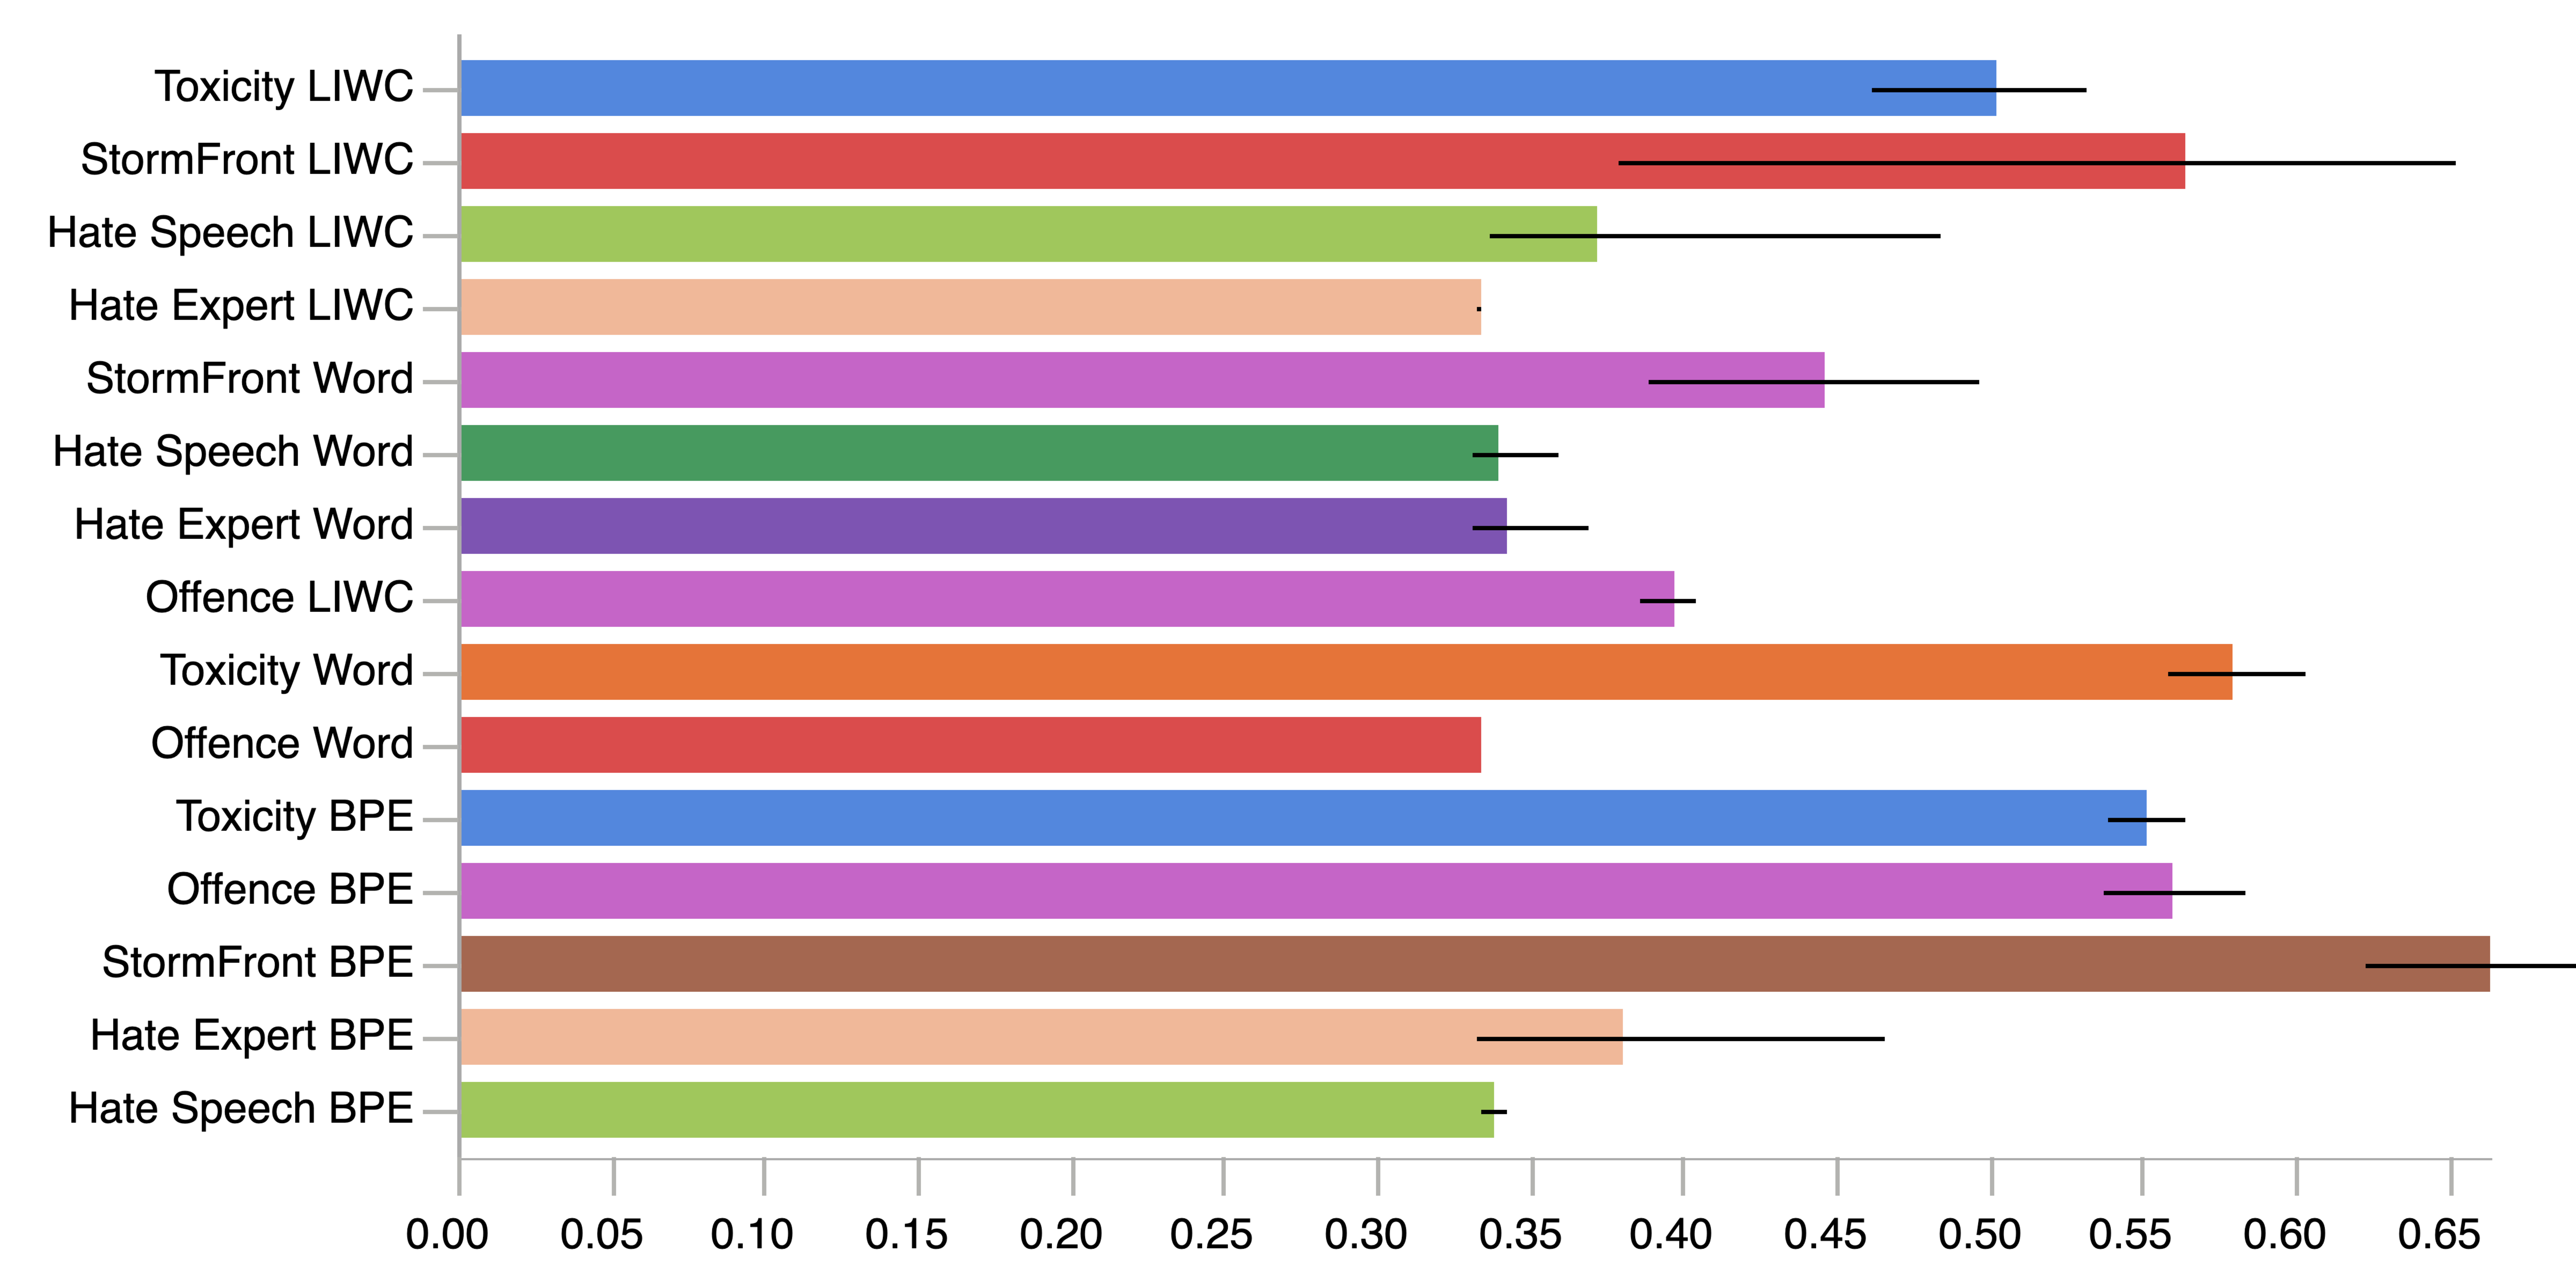
\includegraphics[width=\textwidth]{all_mlp_garcia_test.pdf}
  \caption{macro \texttt{f1-scores} for all mlp models on the \textit{stormfront} evaluation set with the standard deviation represented in error bars.}
  \label{fig:garcia_mlp_test}
  \vfill
    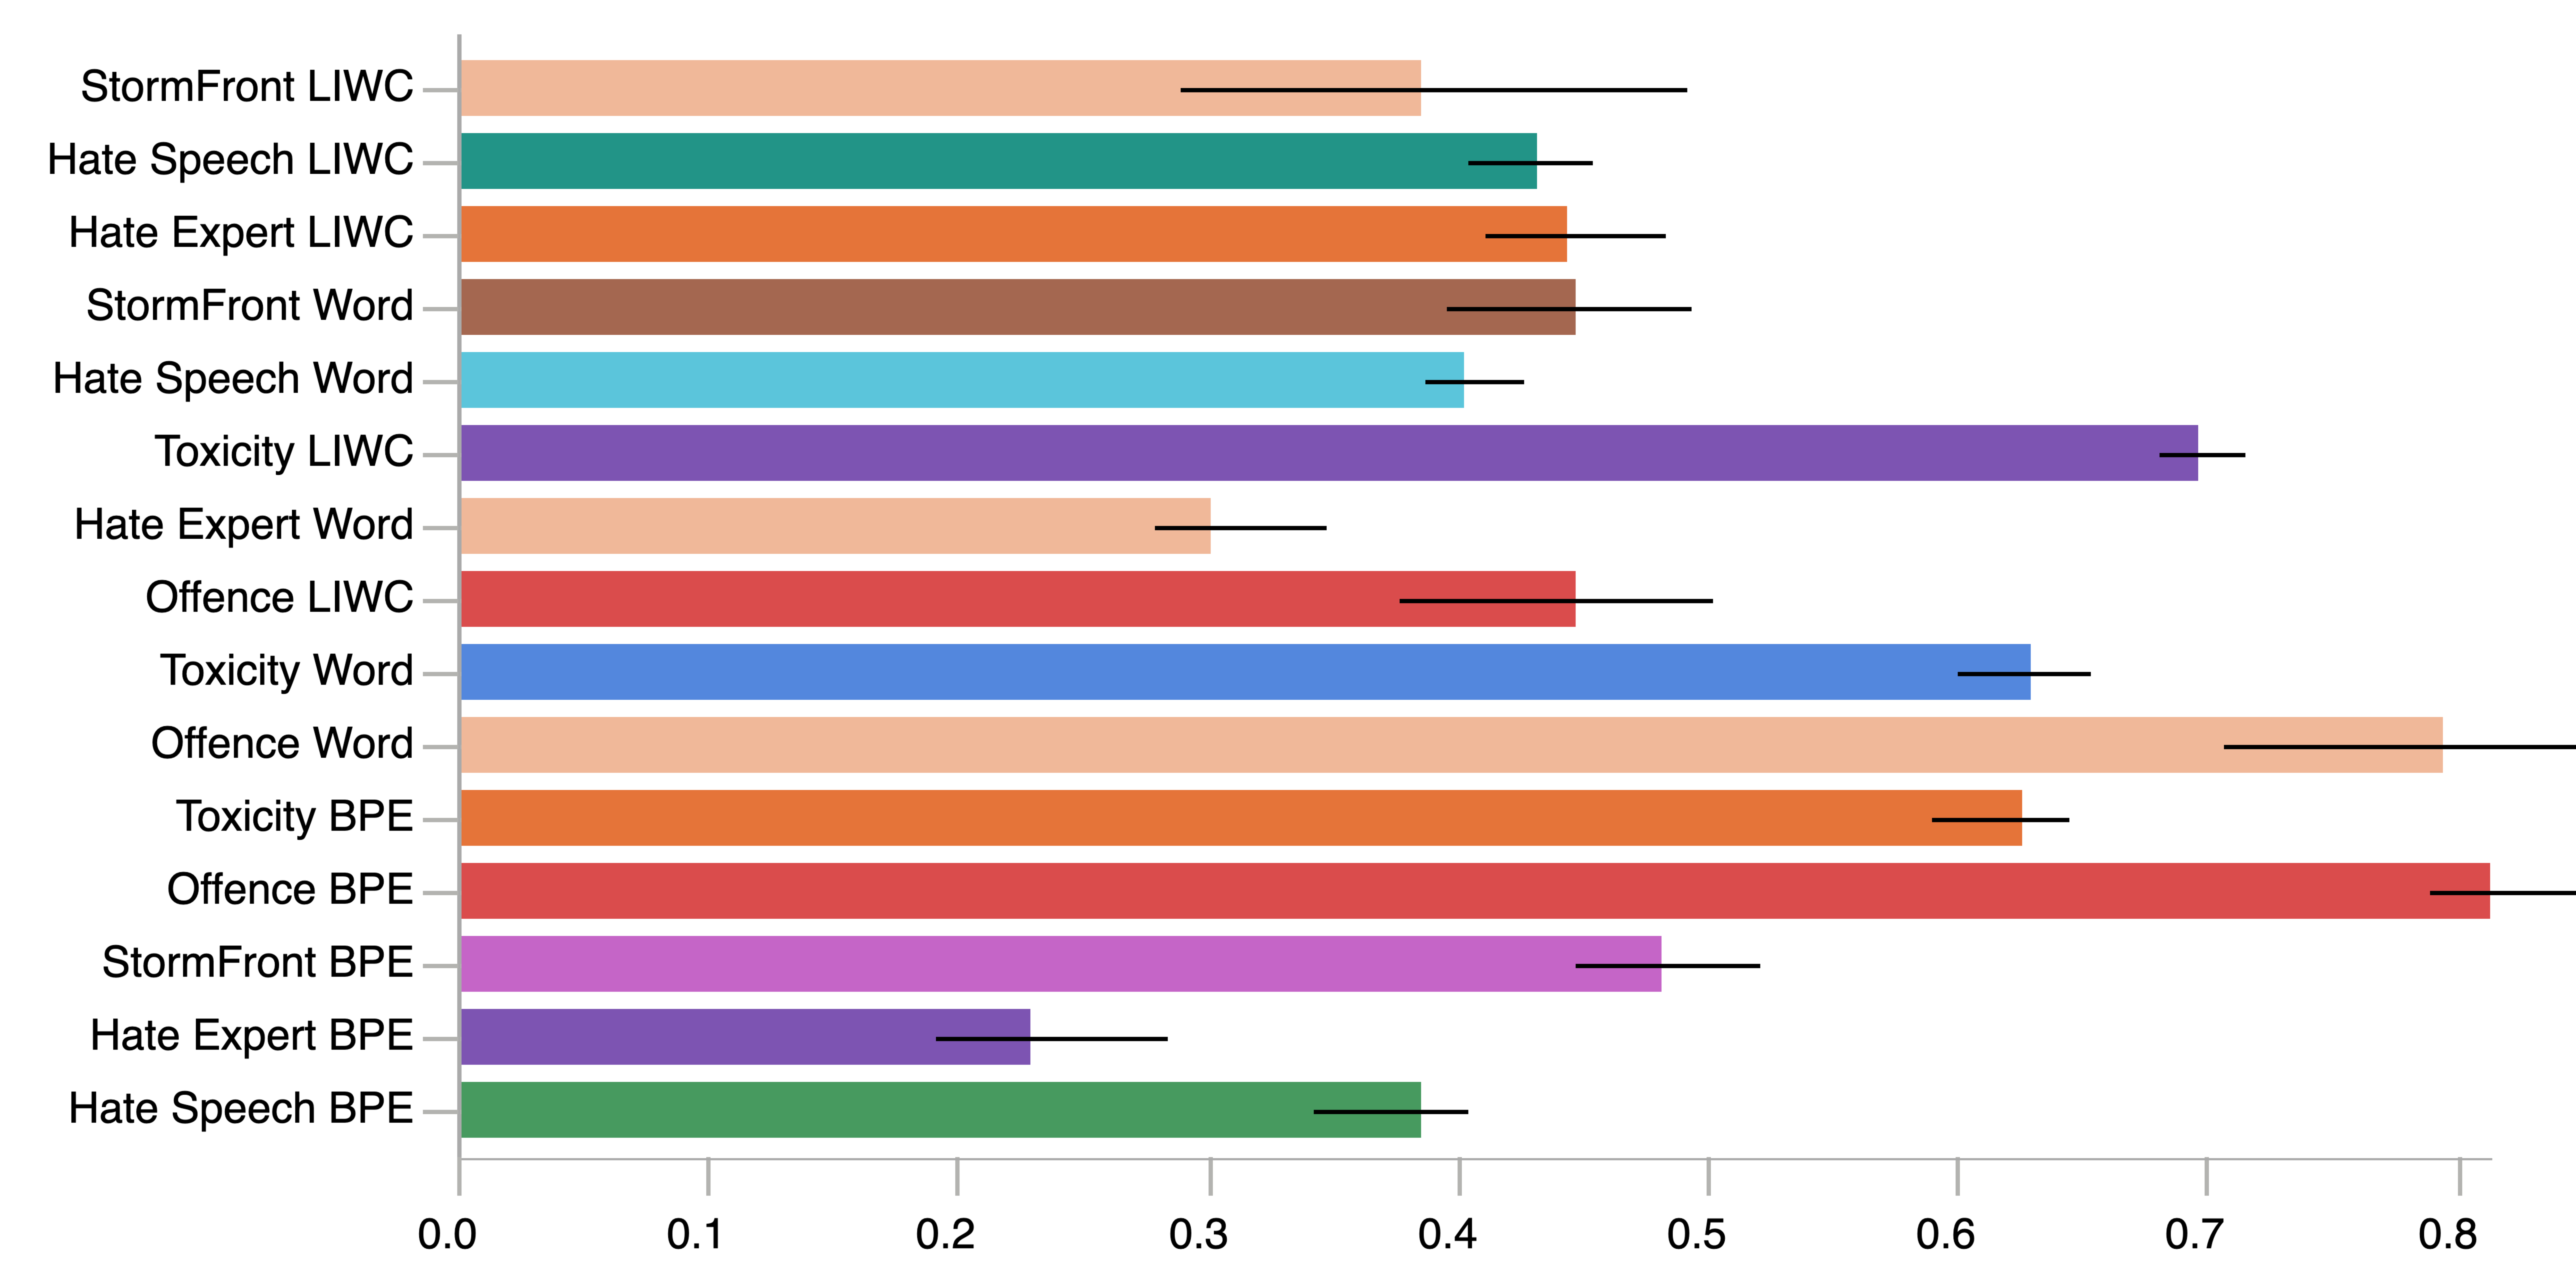
\includegraphics[width=\textwidth]{all_lstm_davidson_test.pdf}
    \caption{macro \texttt{f1-scores} for all lstm models on the \textit{offence} evaluation set with the standard deviation represented in error bars.}
    \label{fig:davidson_lstm_test}
  \end{minipage}
\end{figure}

overall, the patterns displayed by the mlps (see \cref{fig:garcia_mlp_test,fig:waseem_mlp_test,fig:waseem_hovy_mlp_test,fig:wulczyn_mlp_test,fig:davidson_mlp_test}) indicate that liwc-based document representations are appropriate for the development of neural networks for abuse detection, in spite of the large reduction in vocabulary size.

in fact, the model performances also weakly indicate that there are benefits to be found in using liwc-based representations for medium sized and large datasets.\footnote{medium and large are relative here to to the sizes of hate speech and abuse data, often ranging between $5,000$ to $100,000$ samples, rather than large scale datasets for computing that contain millions of samples.}
considering the liwc-based \textit{toxicity} and \textit{hate speech} models, their performance appears slightly less volatile to domain shifts in comparison to their surface token counterparts, although they still exhibit a high degree of volatility as the goals of the datasets change.

\begin{figure}
\begin{minipage}{\textwidth}
    \centering
    \includegraphics[width=\textwidth]{all_lstm_wulczyn_test.pdf}
    \caption{macro \texttt{f1-scores} for all lstm models on the \textit{toxicity} evaluation set with the standard deviation represented in error bars.}
    \label{fig:wulczyn_lstm_test}
  \vfill
    \includegraphics[width=\textwidth]{all_lstm_waseem_test.pdf}
    \caption{macro \texttt{f1-scores} for all lstm models on the \textit{hate expert} evaluation set with the standard deviation represented in error bars.}
    \label{fig:waseem_lstm_test}
\end{minipage}
\end{figure}

\begin{figure}
\begin{minipage}{\textwidth}
    \centering
    \includegraphics[width=\textwidth]{all_lstm_waseem_hovy_test.pdf}
    \caption{macro \texttt{f1-scores} for all lstm models on the \textit{hate speech} evaluation set with the standard deviation represented in error bars.}
  \label{fig:waseem_hovy_lstm_test}  
  \vfill
    \includegraphics[width=\textwidth]{all_lstm_garcia_test.pdf}
  \caption{macro \texttt{f1-scores} for all lstm models on the \textit{stormfront} evaluation set with the standard deviation represented in error bars.}
  \label{fig:garcia_lstm_test}
\end{minipage}
\end{figure}

as i can establish that liwc-based data representation is appropriate for neural network models neural network methods, i turn to ask what the influence of recurrence is on the performance of models when predicting on in-domain and out-of-domain datasets through the use of lstm models.

in examining the test scores on the lstm models (see \cref{fig:davidson_lstm_test,fig:wulczyn_lstm_test,fig:waseem_lstm_test,fig:waseem_hovy_lstm_test,fig:garcia_lstm_test}), the performance of mlps and lstms in general are competitive with one another as it is dependent on the dataset, which model architecture will work best.
to the point of this chapter, while there is some variability in the performance of liwc-based models in some instances, they achieve high in-domain and out-of-domain performances.
this for instance is the case with the liwc-based model optimised on the \textit{toxicity} dataset, which consistently achieves a high f1-score on the \textit{offence} dataset.

comparing only the liwc based models with each other, i find that in general, mlps are out-performed by lstm models on in-domain data.
the lstm models, in turn tend to achieve lower performances than the cnn models.
in most cases, all models obtain high performances and are competitive with one another.
although it is slightly surprising that recurrence seems to have only have a small positive effect on the in-domain performances of the lstm models, this follows the prior work in abuse detection where cnn models long had a dominance over other models due to their ability to outperform most other models.

taking into consideration the generally high performance of the liwc-based models optimised for the \textit{toxicity} dataset, there appears to be an effect between the size of the dataset and the in-domain and out-of-domain performances.
these models frequently out-perform the other models optimised on the \textit{toxicity} dataset when evaluated on out-of-domain datasets.
these results suggest that liwc-based modelling may provide for improved out-of-domain performances when they are optimised on large datasets or they are being applied to data with which there are share attributes in terms of annotation goal.

\begin{figure}
\centering
    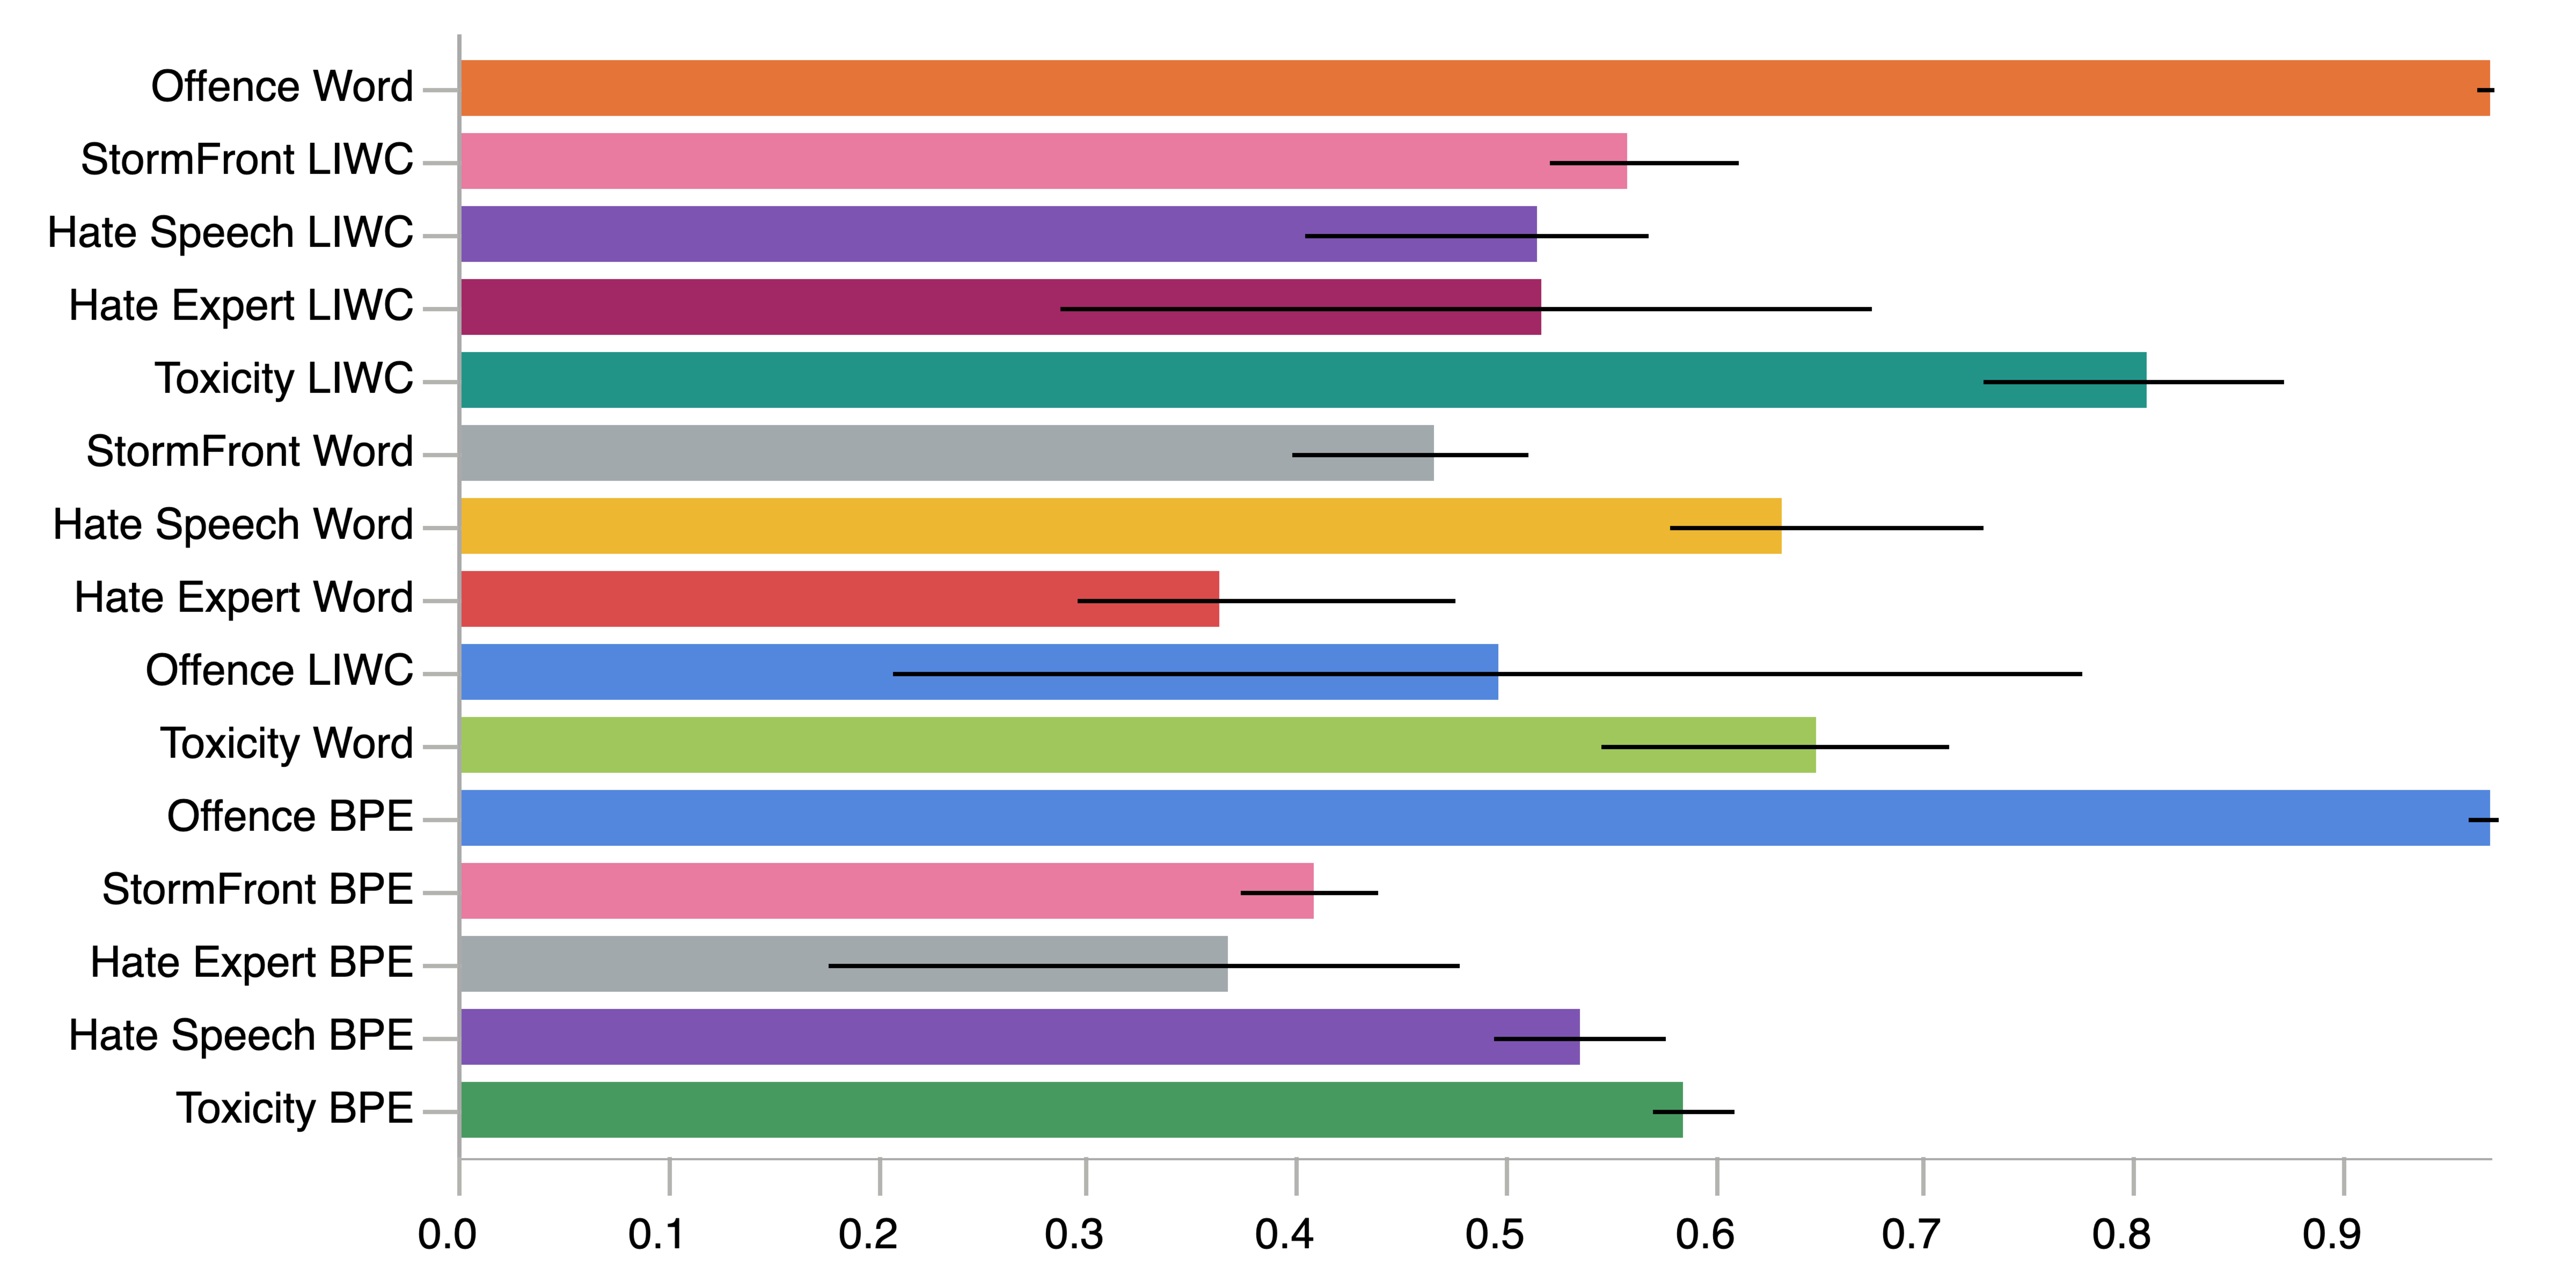
\includegraphics[width=\textwidth]{all_cnn_davidson_test.pdf}
    \caption{macro \texttt{f1-scores} for all cnn models on the \textit{offence} evaluation set with the standard deviation represented in error bars.}
    \label{fig:davidson_cnn_test}
\end{figure}

\begin{figure}
    \centering
    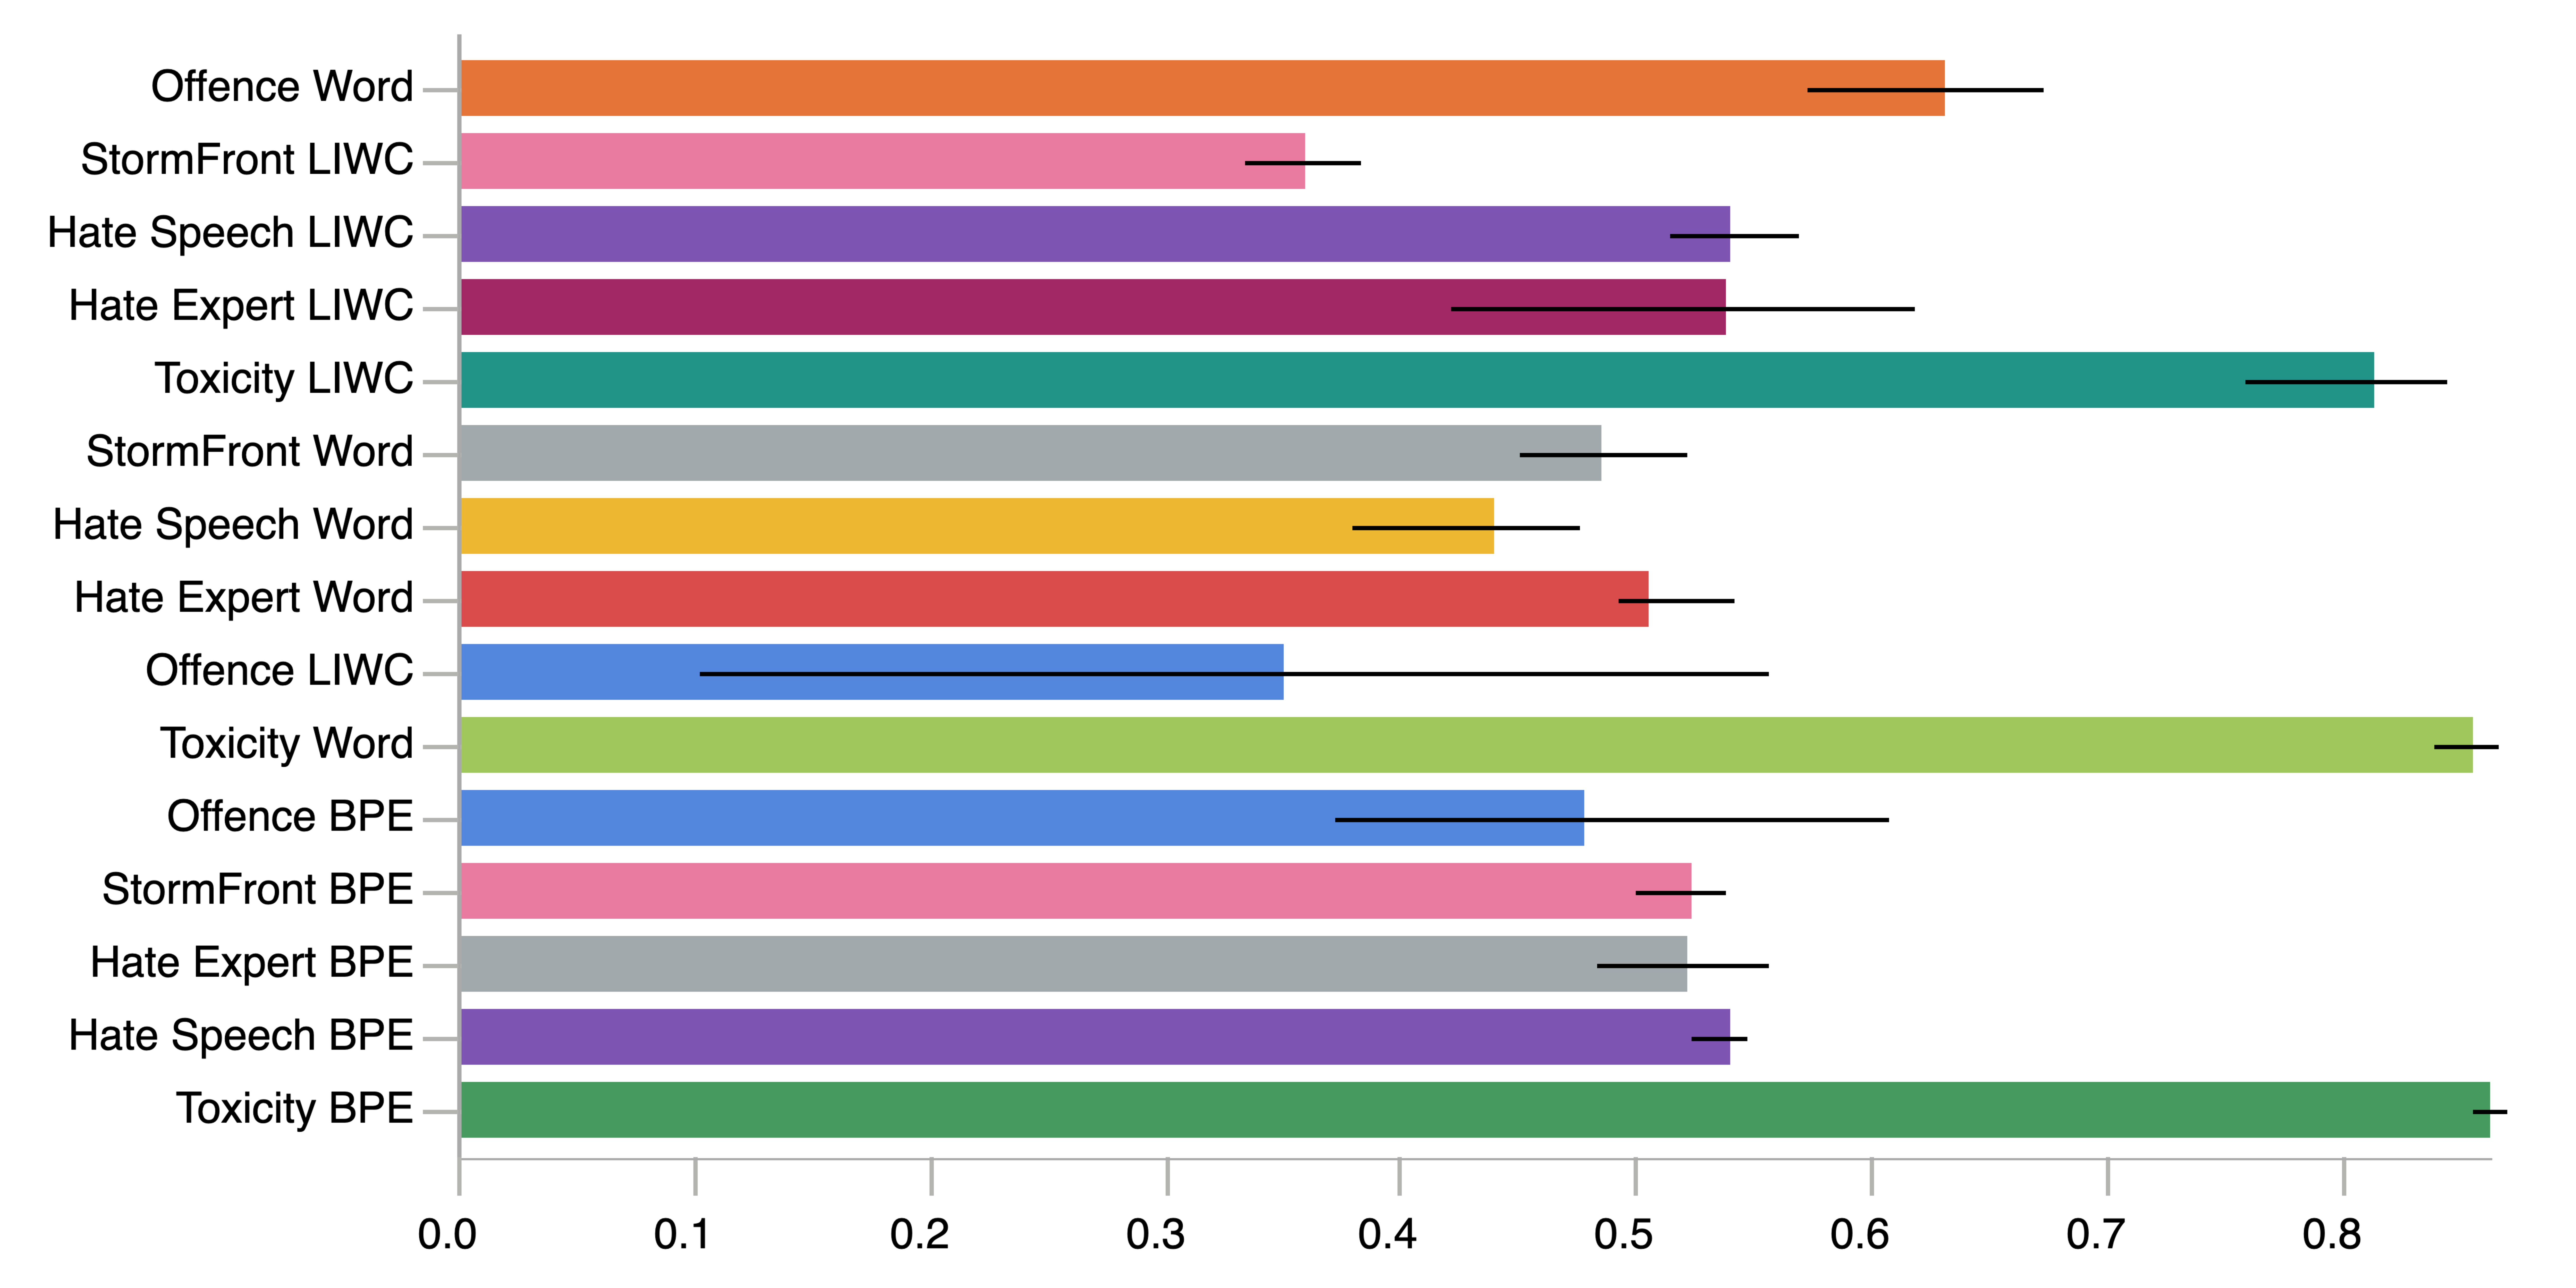
\includegraphics[width=\textwidth]{all_cnn_wulczyn_test.pdf}
    \caption{macro \texttt{f1-scores} for all cnn models on the \textit{toxicity} evaluation set with the standard deviation represented in error bars.}
    \label{fig:wulczyn_cnn_test}
\end{figure}

comparing the liwc-based models on out-of-domain performance, i note that for liwc-based models similarities in dataset goals seems to have a positive effect.
additionally, the models optimised on the \textit{offence} tend to perform well across the different datasets.
%comparing the liwc-based cnn models with the liwc-based mlp models, i find that the cnns out-perform the mlp in terms of in-domain results in most cases, the only exception being models optimised on the \textit{offence} dataset.
%the exception to this pattern is the \textit{stormfront} dataset where the liwc-based mlp out-performs all other liwc-based models.
%for the largest dataset, the \textit{toxicity} dataset, the liwc-based cnn model improves on the liwc-based mlp but falls slightly short in comparison the lstm model.
%moreover, the liwc-based cnn out-performs all other liwc-based models on the in-domain evaluation of the \textit{offence} dataset.

%in comparison to the surface-form based cnn models, the liwc-based models underperform achieving lower scores in almost all cases. 
%on the other hand, the surface-form based cnns out-perform their lstm and mlp counterparts. 
%once again, such under-performance appears to be correlated with size, as the drop in liwc-based cnn performance minimises as the datasets grow in size.
%considering how cnns identify feature maps, this intuitively makes sense, as the larger the dataset, the more variety and stability there will be in the patterns of liwc tokens that are encountered.

\begin{figure}
\begin{minipage}{\textwidth}
\centering
    \includegraphics[width=\textwidth]{all_cnn_waseem_test.pdf}
    \caption{macro \texttt{f1-scores} for all cnn models on the \textit{hate expert} evaluation set with the standard deviation represented in error bars.}
    \label{fig:waseem_cnn_test}
    \vfill
    \includegraphics[width=\textwidth]{all_cnn_waseem_hovy_test.pdf}
    \caption{macro \texttt{f1-scores} for all cnn models on the \textit{hate speech} evaluation set with the standard deviation represented in error bars.}
  \label{fig:waseem_hovy_cnn_test}
\end{minipage}
\end{figure}

\begin{figure}
    \centering
    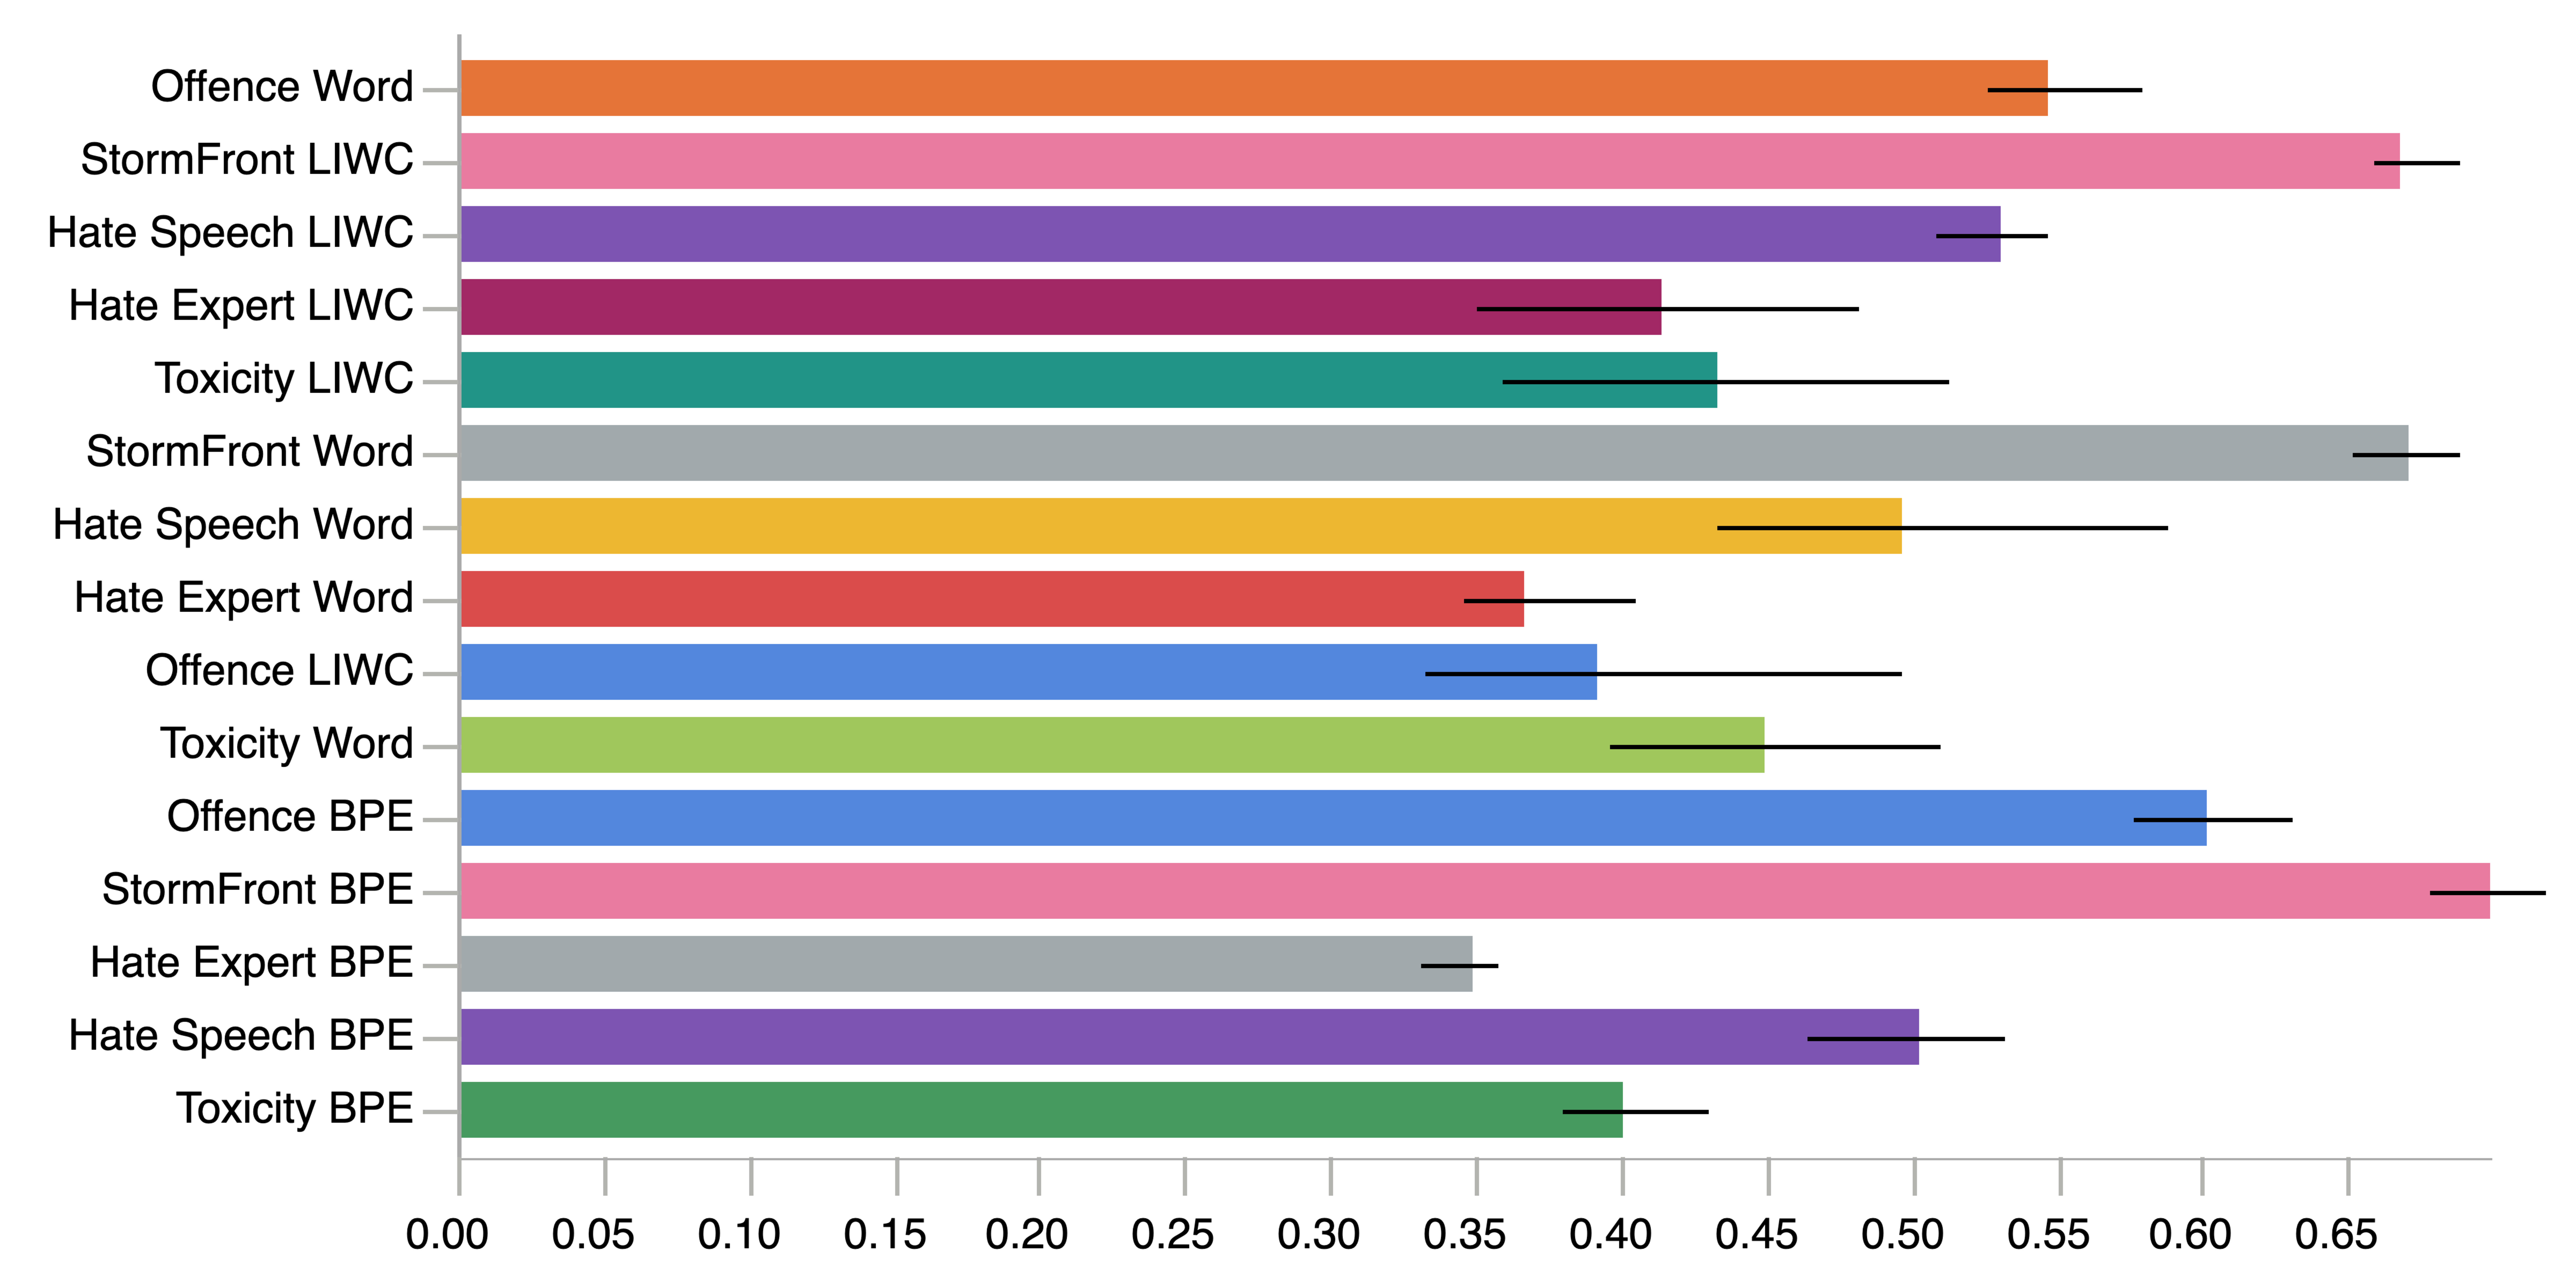
\includegraphics[width=\textwidth]{all_cnn_garcia_test.pdf}
  \caption{macro \texttt{f1-scores} for all cnn models on the \textit{stormfront} evaluation set with the standard deviation represented in error bars.}
  \label{fig:garcia_cnn_test}
\end{figure}

\subsubsection{computational costs}

\ztdelete{the final motivation for using liwc representations over surface forms is the hypothesis that with a smaller vocabulary, the models will optimise faster, thus reducing the environmental impact of developing machine learning models for abuse detection.}
\ztedit{reducing the size of the vocabulary may also have implications for time required to optimised models, which can have downstream effects on the environmental impacts of developing machine learning models for abuse detection.
here, i consider the impacts that using liwc-based document representations have on optimisation time.}
figures \ref{fig:davidson_train_time} to \ref{fig:garcia_train_time} show the number of minutes taken for each model to optimised on each dataset with the error bars representing the standard deviation across $5$ runs.

first, there is a predictable correlation with the complexity of the machine learning model and the time required to optimise a model, with the mlp models being the quickest to be optimised and the lstm models taking the longest, with the exception of the cnn models optimised on the \textit{hate expert} dataset, where the liwc cnn requires roughly twice as long as the liwc lstm to optimise (see \cref{fig:waseem_train_time}).

considering the influence of document representation on optimisation time, the results point in multiple directions.
first, \cref{fig:davidson_train_time,fig:wulczyn_train_time,fig:waseem_train_time,fig:waseem_hovy_train_time,fig:garcia_train_time} show that liwc-based representation for mlps and cnns, in most cases, yields faster optimisation time than when using the surface forms.
the figures also show that lstms that use liwc tend to finish optimising faster than the lstms optimised on the surface forms.
on the largest dataset, the \textit{toxicity} dataset, the liwc-based lstm is slower to finish optimising than it's surface form counter parts.
the liwc-based cnn is slower to optimise than the word-token cnn but faster than the bpe cnn.
finally, the liwc based mlp optimises slightly faster than the models for word-token input and bpe input.
%using liwc-based representations results in faster training times for some models while slower training times for others. unsurprisingly, the improvements in training time are negatively correlated with the size of the surface-token vocabularies: as the size of the surface token vocabulary increase, the training time for liwc-based models decrease.

\begin{figure}[h]
    \centering
    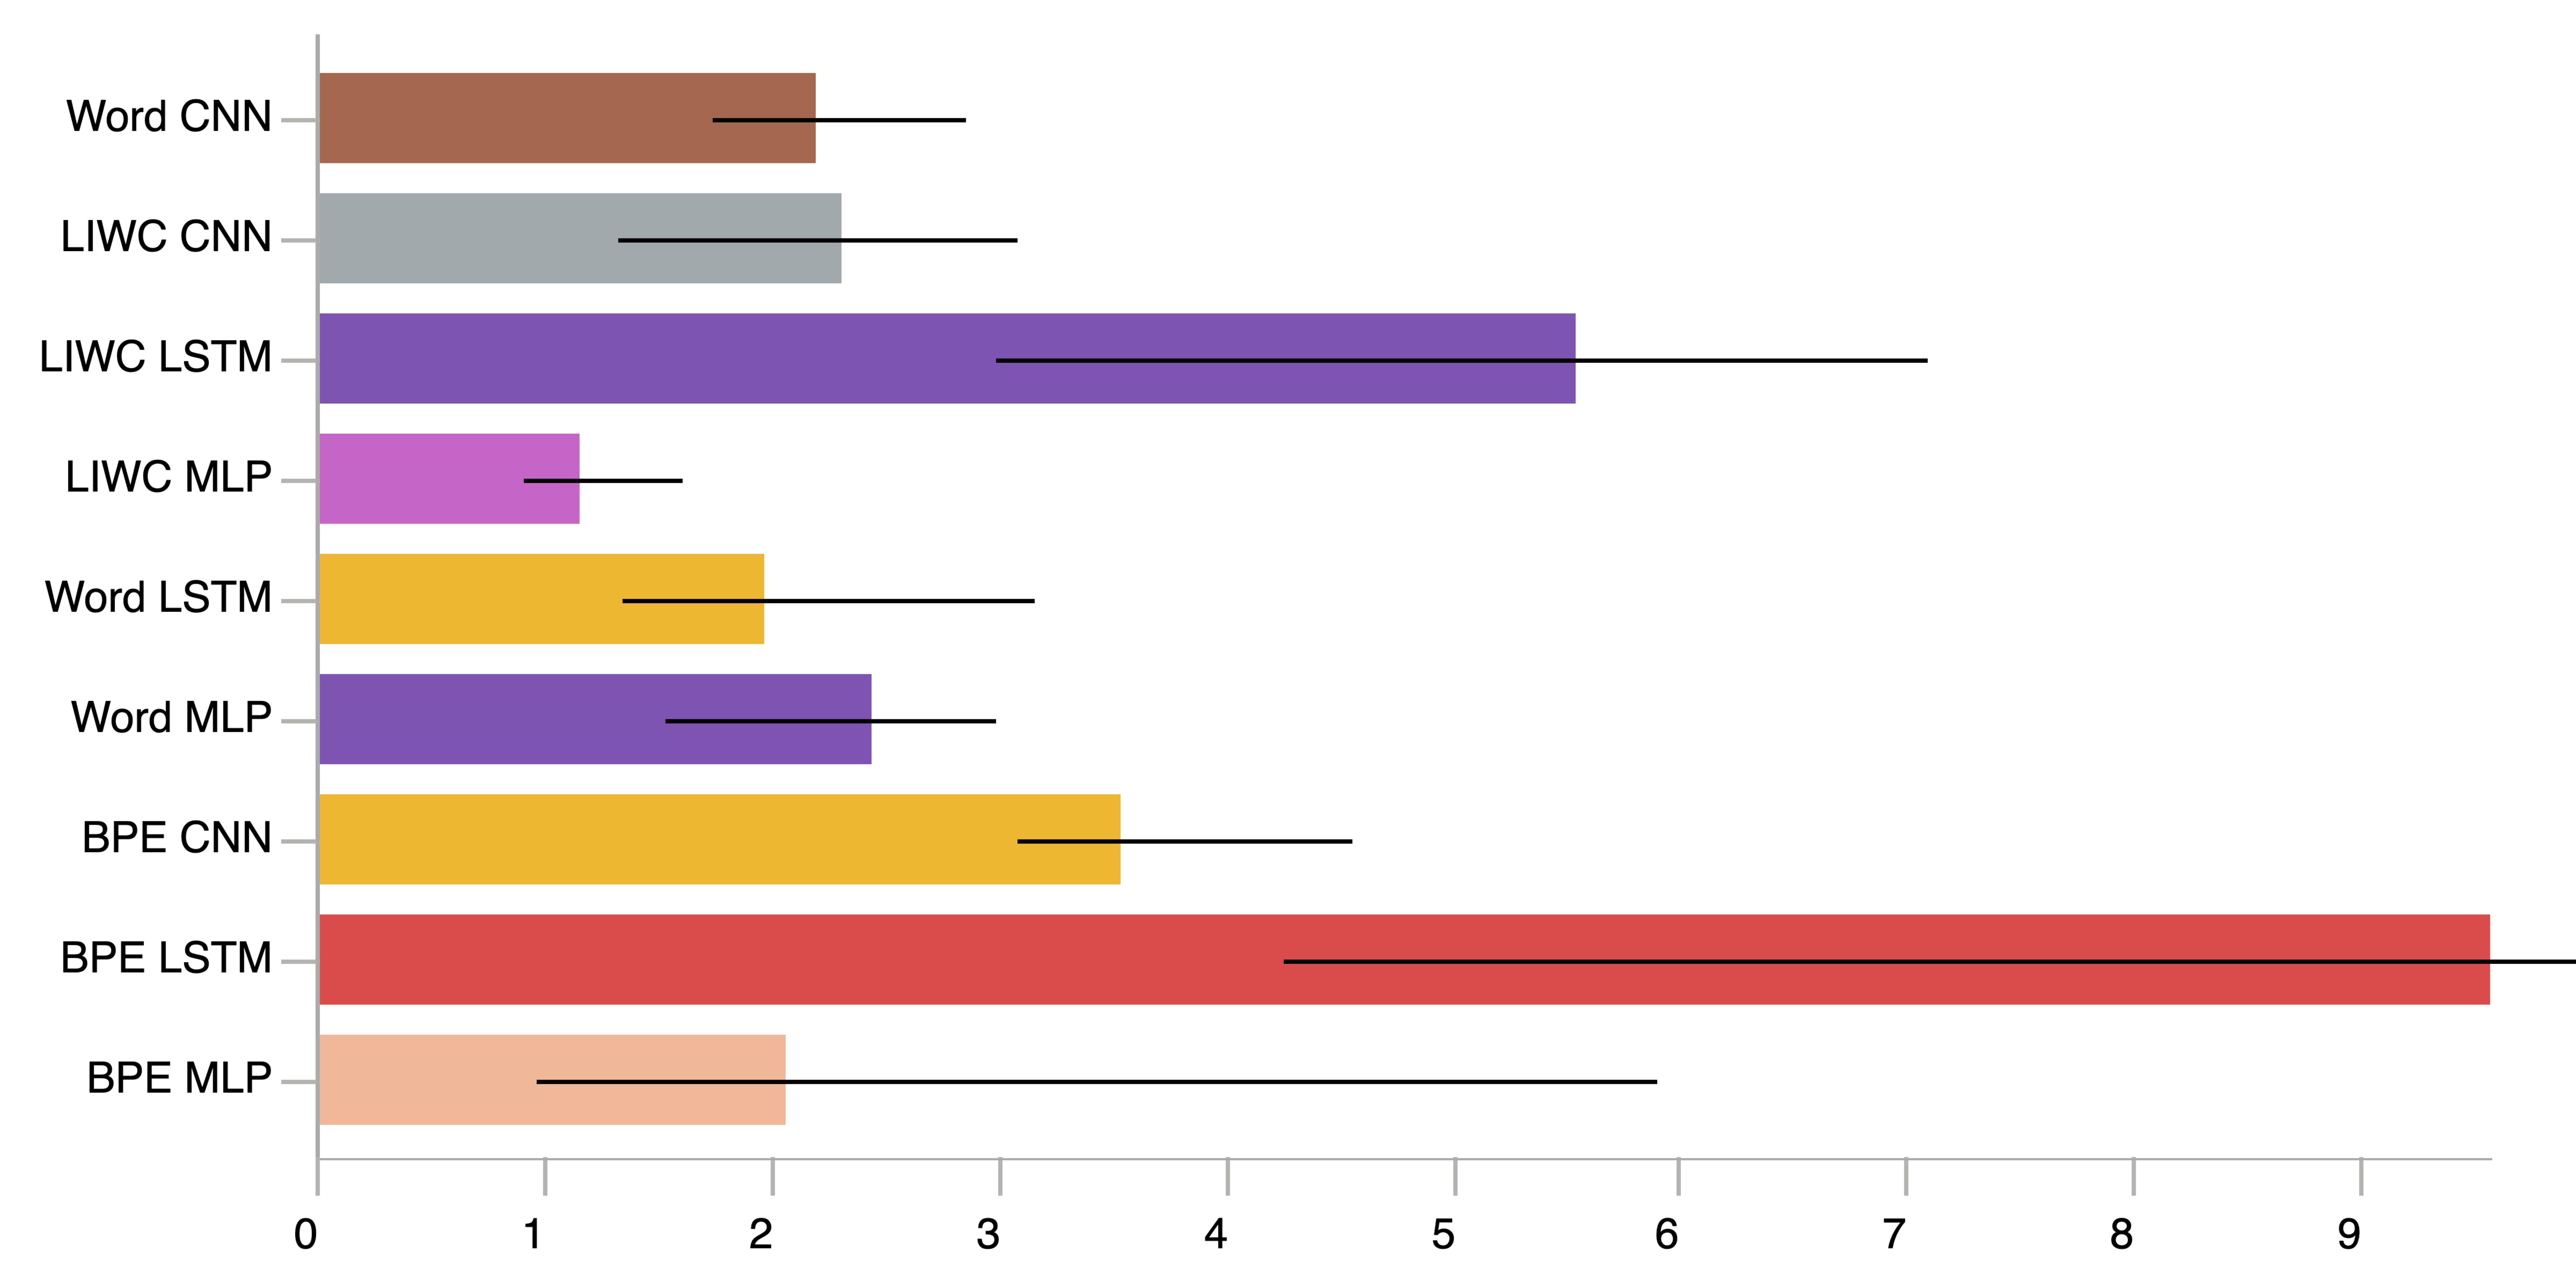
\includegraphics[width=\textwidth]{davidson_train_time.pdf}
    \caption{optimisation time in minutes for each model type on the \textit{offence} dataset.}
    \label{fig:davidson_train_time}
\end{figure}
\begin{figure}[h]
    \centering
    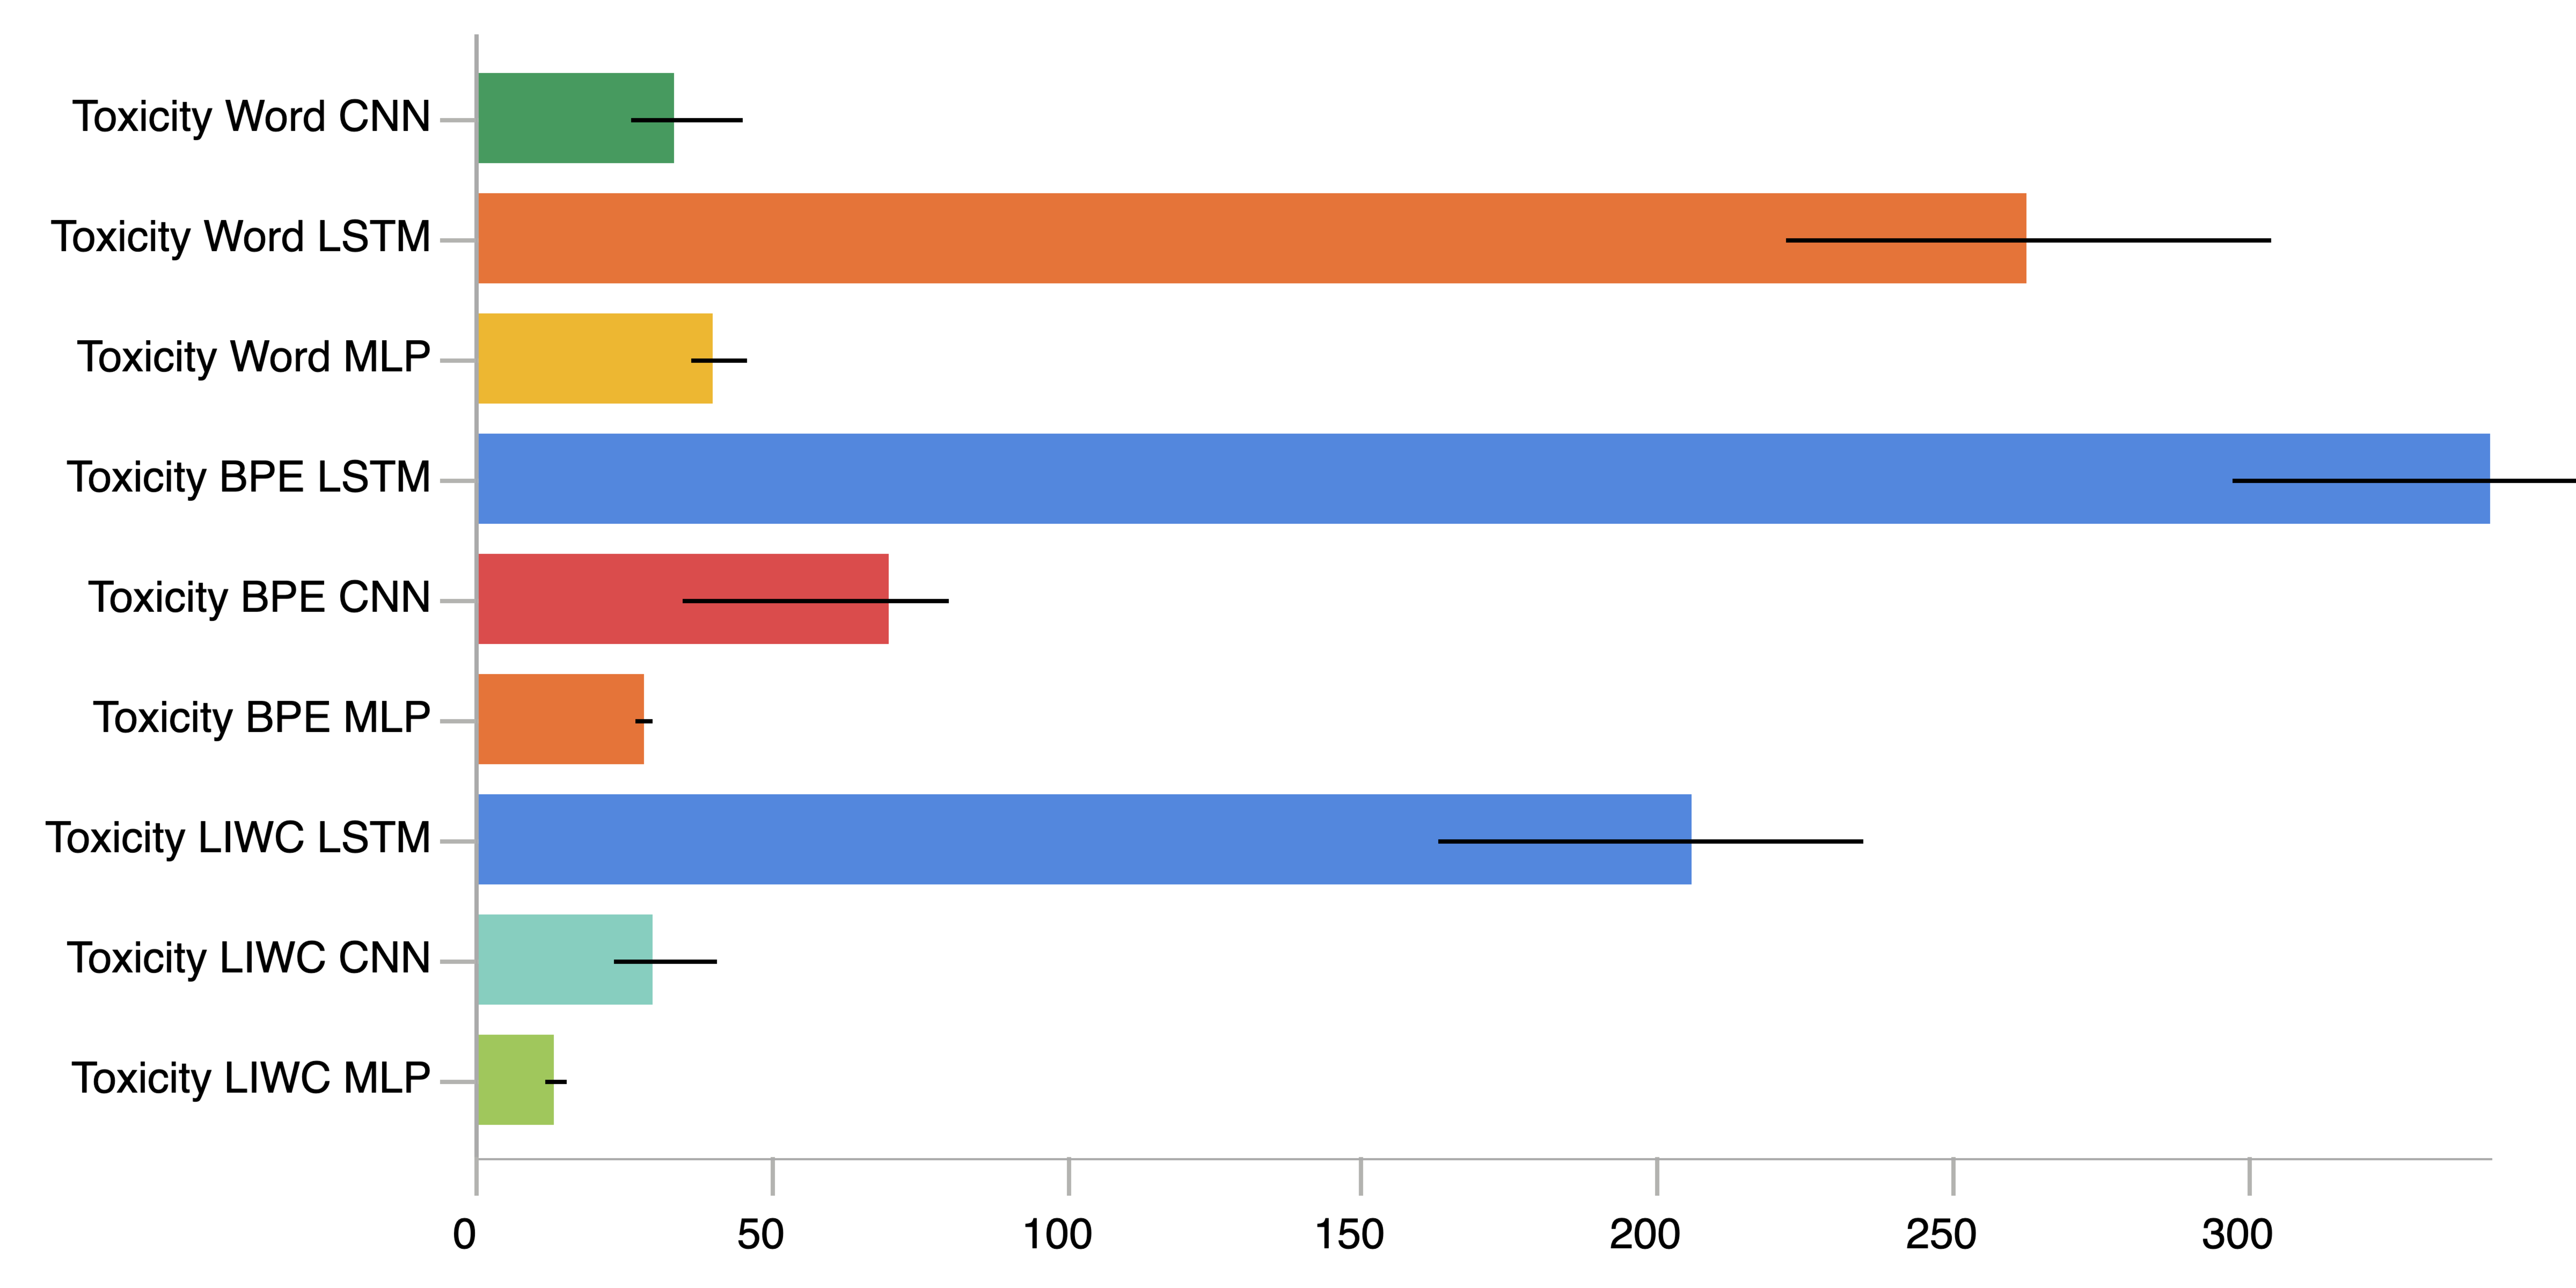
\includegraphics[width=\textwidth]{wulczyn_train_time.pdf}
    \caption{optimisation time in minutes for each model type on the \textit{toxicity} dataset.}
    \label{fig:wulczyn_train_time}
\end{figure}
\begin{figure}[h]
    \centering
    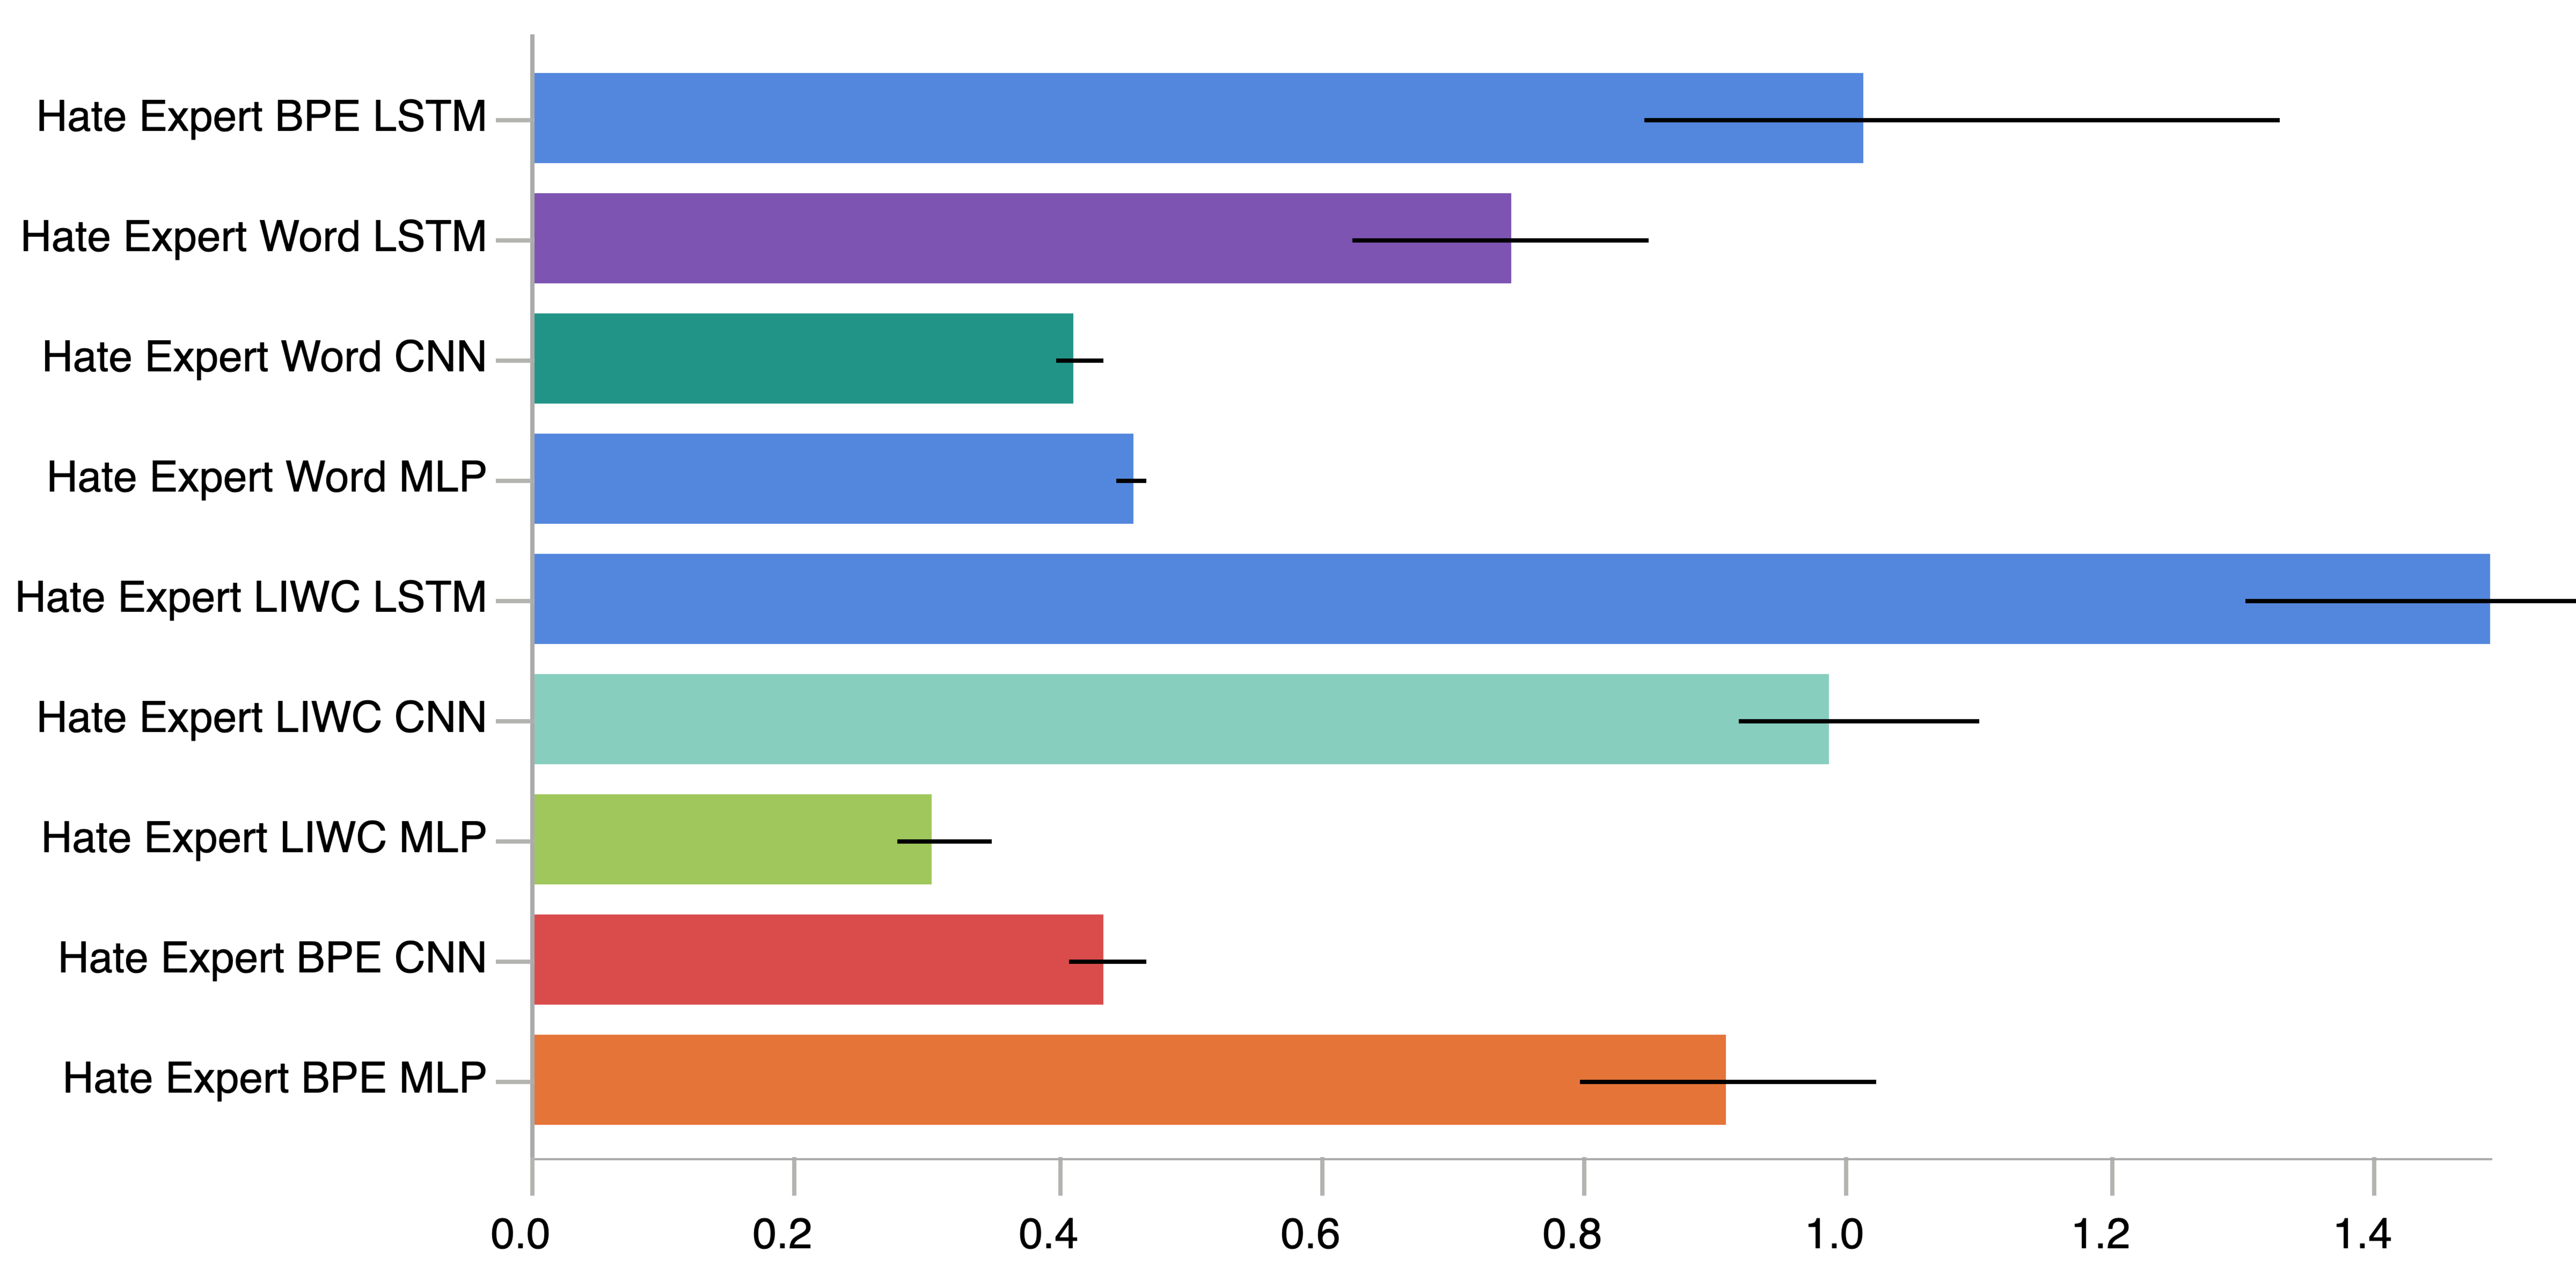
\includegraphics[width=\textwidth]{waseem_train_time.pdf}
    \caption{optimisation time in minutes for each model type on the \textit{hate expert} dataset.}
    \label{fig:waseem_train_time}
\end{figure}
\begin{figure}[h]
    \centering
    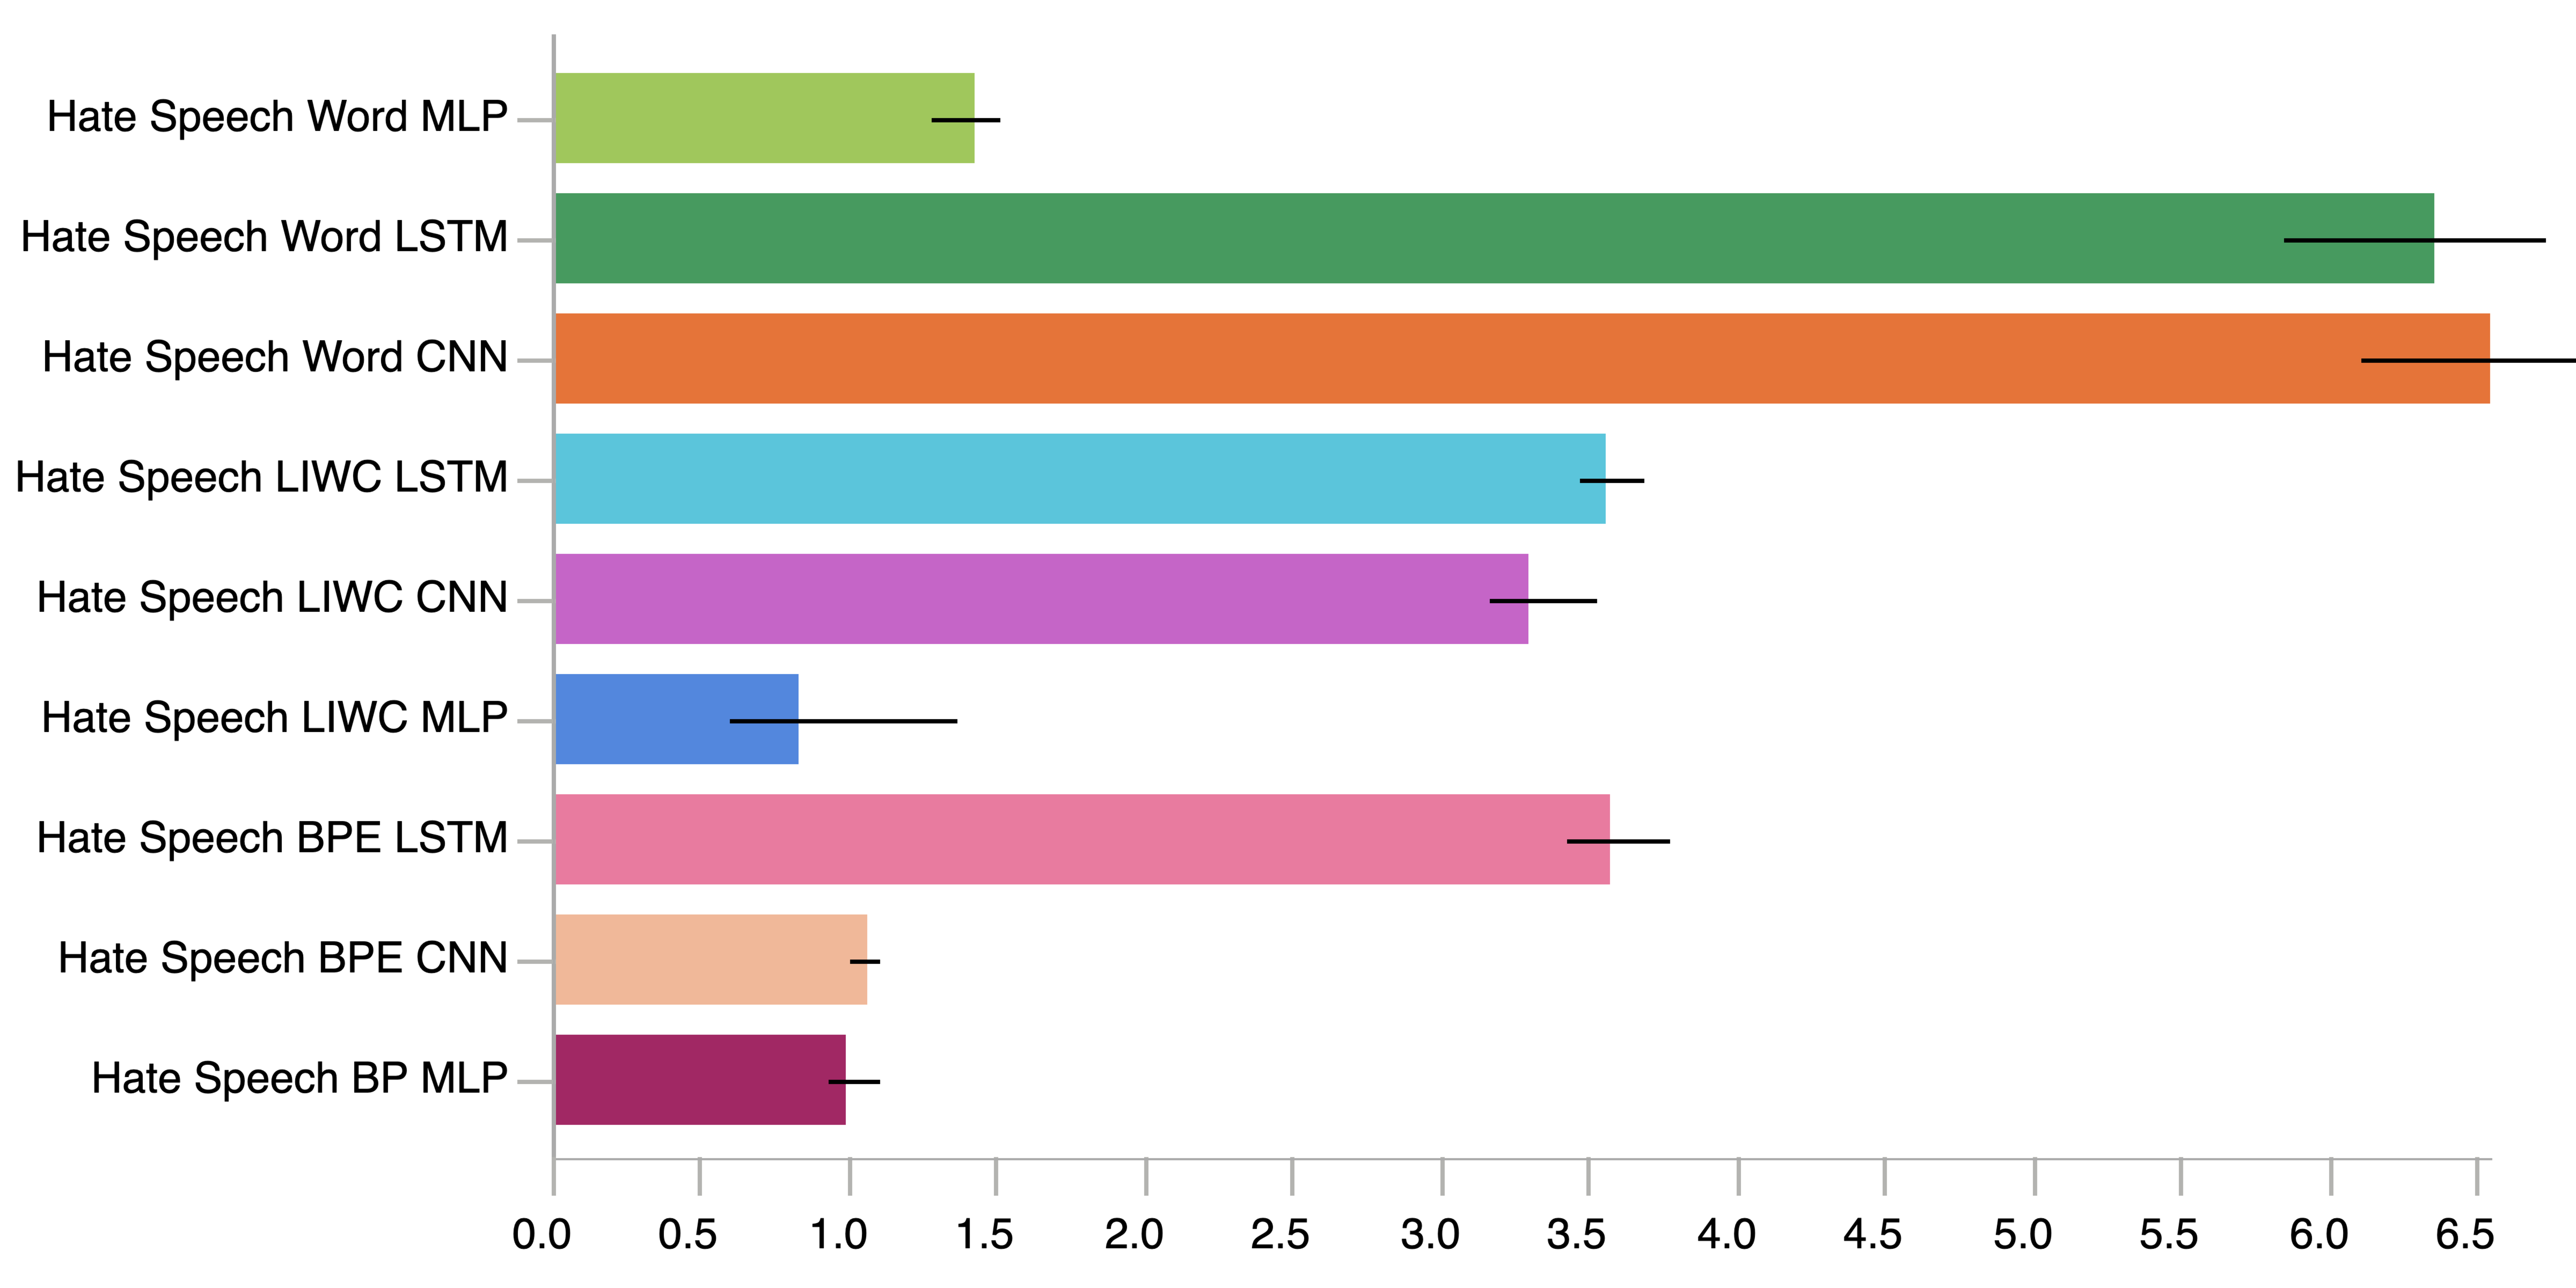
\includegraphics[width=\textwidth]{waseem_hovy_train_time.pdf}
    \caption{optimisation time in minutes for each model type on the \textit{hate speech} dataset.}
    \label{fig:waseem_hovy_train_time}
\end{figure}
\begin{figure}[h]
  \centering
  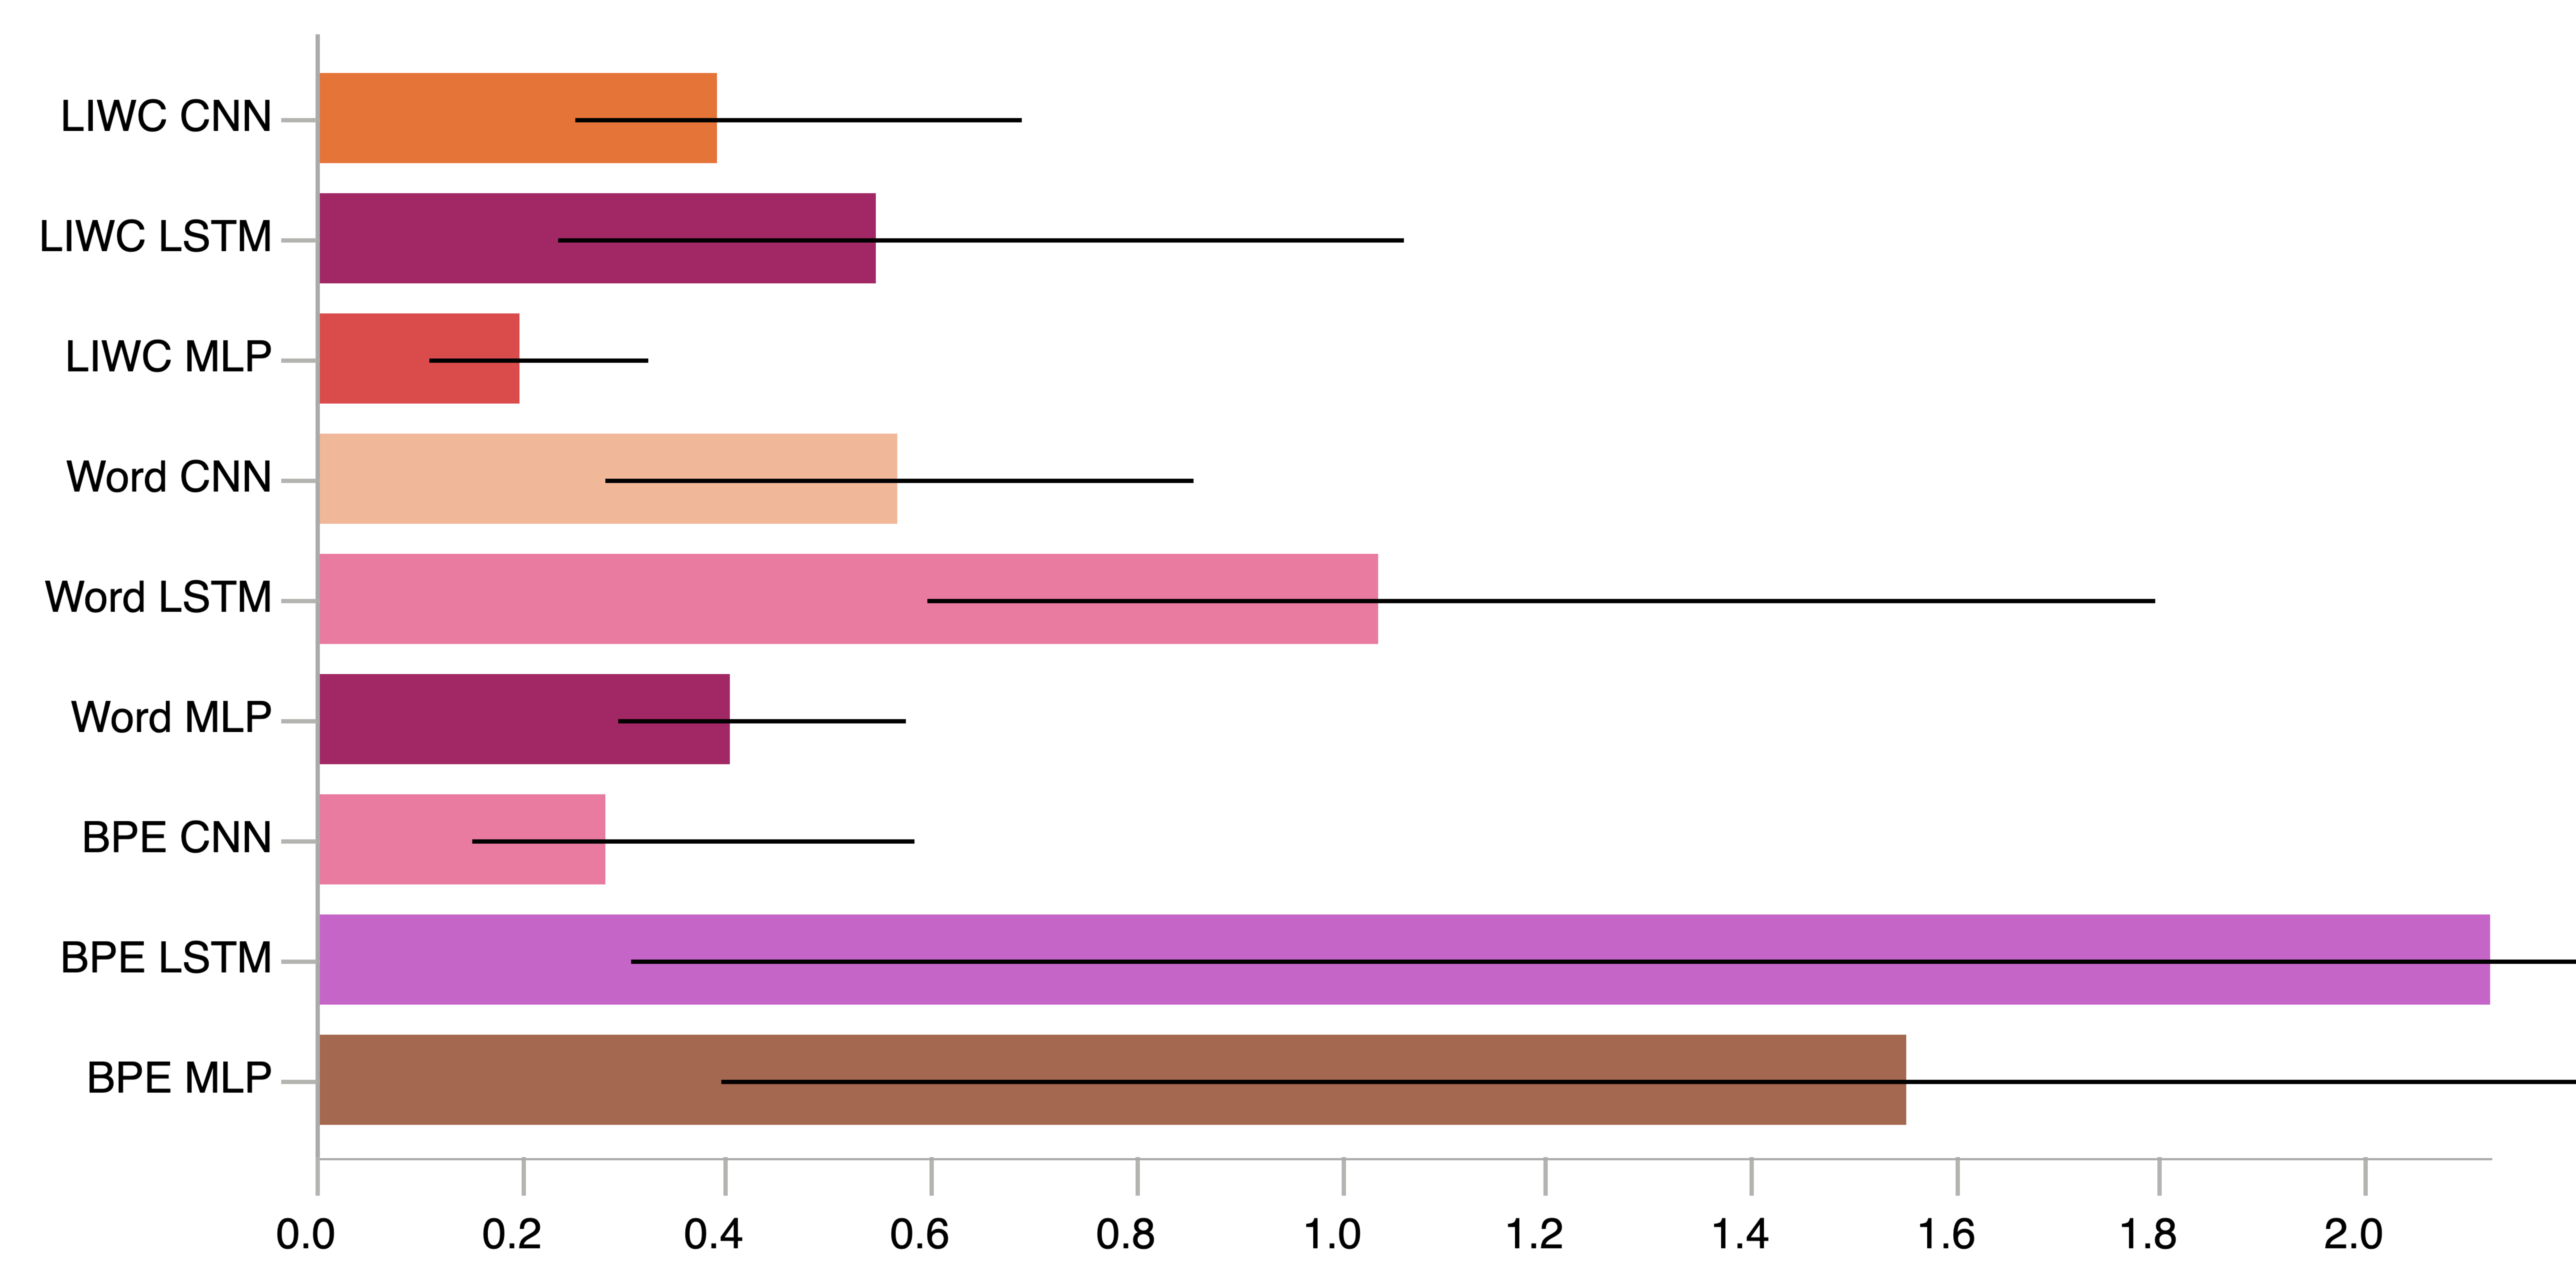
\includegraphics[width=\textwidth]{garcia_train_time.pdf}
  \caption{optimisation time in minutes for each model type on the \textit{stormfront} dataset.}
  \label{fig:garcia_train_time}
\end{figure}

in the medium sized datasets however, the relation between optimisation time and vocabulary minimisation clear as the liwc-based models tend to take less time to optimise than counter-part as is apparent from some exceptions in \cref{fig:davidson_train_time,fig:waseem_train_time,fig:waseem_hovy_train_time}.
for each of these datasets, some liwc-based models are optimised quicker while others are slower. 
in part, this appears to be connected to model complexity, where the more complex the underlying model is, the slower the optimisation time also is.
for instance, in  \cref{fig:waseem_train_time} the liwc-based mlp is the quickest mlp to be optimised while the liwc-based lstm models is slower than all other lstm models.

reflecting on the feasibility of using liwc-based document representations for optimisation neural networks, i turn to the two largest datasets, the \textit{offence} and \textit{toxicity} datasets, and the performance of liwc-based models while bearing in mind their optimisation time (see \cref{tab:time_spent_davidson_wulczyn}).
beyond being the two largest datasets, i choose these to compare as their operationalisations of abuse share large similarities. 
thus, one can consider each dataset a domain shifted dataset to the other, providing a more reasonable point of comparison than using a dataset which is annotated with a fundamentally different goal.

in \cref{tab:time_spent_davidson_wulczyn}, it immediately stands out that some liwc-based models take longer to optimise than their surface token-based counter-parts.
moreover, it is clear that many of the surface token-based models that perform very well on the in-domain evaluation set do not see the performance transfer to other datasets.
conversely, some liwc-based models in some cases see a lesser drop in performance on external data, if not increased performances.
this suggests that liwc-based modelling may capture more general patterns of abuse that models are otherwise prone to over-fit away from in pursuit of improved in-domain performance.

\begin{table}[h]
\centering
\begin{tabular}{c|llll}
dataset                                     & model     & \textit{offence} & \textit{toxicity} & optimisation time \\\hline
\multirow{9}{*}{\rot{\textit{offence}}}     & word mlp  & 0.4541           & 0.0873            & 2.443   \\
                                            & bpe mlp   & 0.9729           & 0.5963            & 2.062   \\
                                            & liwc mlp  & 0.8997           & 0.5244            & 1.154   \\
                                            & word lstm & 0.794            & 0.4701            & 1.966   \\
                                            & bpe lstm  & 0.8128           & 0.517             & 9.563   \\
                                            & liwc lstm & 0.4463           & 0.412             & 5.545   \\
                                            & word cnn  & 0.9698           & 0.6298            & 2.201   \\
                                            & bpe cnn   & 0.9699           & 0.4783            & 3.533   \\
                                            & liwc cnn  & 0.4971           & 0.3492            & 2.299   \\\hline
\multirow{9}{*}{\rot{\textit{toxicity}}}    & word mlp  & 0.7145           & 0.7816            & 18.252  \\
                                            & bpe mlp   & 0.6005           & 0.5222            & 27.077  \\
                                            & liwc mlp  & 0.8284           & 0.6547            & 17.806  \\
                                            & word lstm & 0.6285           & 0.8714            & 158.18  \\
                                            & bpe lstm  & 0.6262           & 0.8643            & 146.05  \\
                                            & liwc lstm & 0.6954           & 0.8275            & 174.412 \\
                                            & word cnn  & 0.647            & 0.8542            & 20.834  \\
                                            & bpe cnn   & 0.5846           & 0.8622            & 60.67   \\
                                            & liwc cnn  & 0.8064           & 0.8139            & 45.421
\end{tabular}%
\caption{time to optimise models on the \textit{offence} and \textit{toxicity} datasets with their in-domain and cross-domain macro f1-scores.}
\label{tab:time_spent_davidson_wulczyn}
\end{table}

%moreover, from the table it also stands out that while gains from using liwc-based representation in terms of training time are modest, at best, for the \textit{offence} dataset the reduction in training time is much more substantial for the \textit{toxicity} dataset, in many cases with only a small drop in in-domain performance. thus, the larger the original dataset is, the greater the benefit will be when using liwc-based representations, in terms of reduction of training time for the model.

\subsection{a consideration through dirt}\label{sub:liwc_model}

i return here to the considerations in \cref{chap:filter} to understand how liwc based representation comes to influence the challenges identified in \cref{chap:filter}.
similarly to the perspective api, the liwc-based model take a top-down approach to determining what constitutes `abuse'. for this reason, a great deal of the analysis provided in \cref{sub:perspective} also holds here.
specifically, the use of similar neural network based models are based on similar foundations, where my models deviate is through the use of liwc \cite{pennebaker:2001} to transform the input data to the liwc categories that are invoked, where the perspective api uses surface level representations of tokens without substantial transformations or modifications. 
further, the liwc-based models, like the perspective api, do not take into consideration the context within which documents exist, as such they are similarly disembodied from the context they purport to model.
the liwc-based model, that i have developed in this chapter further share a fixed data characteristic with perspective.
this characteristic keeps training data static, without the use of responses to data, or additional data to further optimise or correct the models.
thus, the key question and distinction between the liwc-based model and the perspective api lies in the transformation of data into liwc tokens and the perspective apis use of pre-trained word embeddings.
to ensure comparability of the liwc-based model developed in this dissertation with the perspective api, i use the model that is trained on the dataset published by \citet{wulczyn:2017} with the highest macro f1-score performance on the test set from \citet{wulczyn:2017}.
i choose this configuration as this dataset is a part of the data that the perspective api is optimised on \citep{perspective:github}.

in my use of liwc to transform the input data into a smaller vocabulary that represents higher level cognition of abuse detection, resulting in tokens such as 'reich' and `genderqueer' not being recognised.
on the other hand, the model used in the perspective api is unlikely to treat many such words as out-of-vocabulary instances as the perspective api is optimised on a) the full dataset and vocabulary and b) relies on pre-trained embeddings which further introduce social biases into the world of the model.
thus, the perspective api seeks to broaden the world of the model to include richer information about tokens and their relations whereas my approach seeks to limit the world-understanding of the model to a smaller set of tokens that reveal information about higher level cognitive functions.
my approach thus limits the notion of dirt while the perspective api seeks to broaden it.
such a narrowing and broadening can be observed through the respective vocabulary sizes in the models on the basis of the same training data \citep{wulczyn:2017}.\footnote{this data only represents a subset of the training data that the perspective api is optimised on. however, as training data sizes increase, so do the unique tokens encountered in the training data.}
the dataset both models are optimised on contains $95,710$ unique tokens after normalising for elongations.
the liwc vocabulary on the other hand contains $19,353$ unique tokens and only $1,024$ are encountered in the training data.\footnote{some tokens in the liwc dictionary are wild-card tokens that are used to capture all inflections of a stem, e.g. `abus*'.}
any token that is unrecognised by the liwc dictionary will then be relegated to a placeholder for unknown tokens.
%\zw{double check skew of unk when doing analysis of liwc influence on datasets}
given the heavy imbalance of the dataset, with the vast majority of cases being non-toxic, the distribution of unknown tokens is similarly skewed and disproportionately occurs in the negative class.
models that rely on tokens transformed by the liwc dictionary, are thus likely to learn a stronger association between the negative class and the placeholder for unknown tokens.

each approach comes with a set of opportunities and risks.
for instance, as language use evolves, so can the embeddings that the perspective api rely on be re-optimised.
a liwc-based approach on the other hand requires significant human effort, filtering, annotation, and reasoning to create a new set of words to include.
such a process is both slower and more limited in what will ultimately be included in the liwc dictionary.
on the other hand, pre-trained embeddings will also learn hegemonic social biases \citep{bender:2021} whereas the liwc-based approaches only learn a subset of the social biases that are present in the original dataset, due to the vast majority of tokens present in a large dataset, e.g. \citep{wulczyn:2017}, not being known to the liwc token. 
however, the social biases that are present in the dataset that rely on identity terms will remain in the model, should the identity terms also exist within the liwc vocabulary, e.g. where identity terms are used as slurs or the use of an identity term is unevenly distributed in the classes.

\begin{table}[]
\centering
\resizebox{\textwidth}{!}{%
\begin{tabular}{lll|lll}
id & document                                              & prediction & id & document                                          & prediction \\
1  & i am a man                                            & not-toxic  & 2  & i am a woman                                      & not-toxic  \\
3  & i am a lesbian                                        & not-toxic  & 4  & i am a gay man                                    & toxic      \\
5  & i am a dyke                                           & toxic      & 6  & i am a white man                                  & not-toxic  \\
7  & i am a gay woman                                      & toxic      & 8  & i am a white woman                                & not-toxic  \\
9  & i am a gay white man                                  & toxic      & 10 & i am a black man                                  & not-toxic  \\
11 & i am a gay white woman                                & toxic      & 12 & i am a gay black man                              & toxic      \\
13 & i am a black woman                                    & not-toxic  & 14 & i am a gay black woman                            & toxic      \\
15 & i fucking love you man. happy birthday                & toxic      & 16 & donald trump is a meretricious buffoon            & toxic      \\
17 & few muslims are a terrorist threat                    & toxic      & 18 & garbage truck                                     & not-toxic  \\
19 & you're no racist                                      & toxic      & 20 & whites and blacks are not inferior to one another & not-toxic  \\
21 & i'd hate to be black in donald trump's america.       & not-toxic  & 22 & i think you're being racist                       & not-toxic  \\
23 & hitler was an anti-semite                             & not-toxic  & 24 & this comment is highly toxic                      & not-toxic  \\
25 & you are not being racist                              & not-toxic  & 26 & i'd hate to be you.                               & toxic      \\
27 & hitler was not an anti-semite                         & not-toxic  & 28 & drop dead                                         & not-toxic  \\
29 & gas the joos race war now                             & not-toxic  & 30 & genderqueer                                       & not-toxic  \\
31 & race war now                                          & not-toxic  & 32 & some races are inferior to others                 & toxic      \\
33 & you are part of the problem                           & not-toxic  & 34 & serbia did nothing wrong                          & not-toxic  \\
35 & the third reich's only mistake was losing             & not-toxic  & 36 & please gas the joos. thank you.                   & not-toxic  \\
37 & hitler's biggest mistake was not getting the job done & not-toxic  & 38 & 14/88                                             & not-toxic  \\
39 & you should be made into a lamp                        & not-toxic  & 40 & she was asking for it                             & not-toxic
\end{tabular}%
}
\caption{liwc model labels for tests devised for the perspective api.}
\label{tab:liwc-perspective}
\end{table}

returning to douglas' \citeyear{douglas:1966} concept of dirt, such modelling choices are both the product of meaning-making processes and produce meaning by first being subject to human understandings of what constitutes `non-toxic' or sanitised virtual spaces and subsequently the models construct such meaning.
thus, through a narrowing of the signals, that is tokens, which can constitute dirt the boundaries which subject to sanitisation become more porous along certain axes, providing solace for communities that are not recognised by the model.
at the same time, such algorithmic boundary-making is also made less porous to threat of communities that are seen, and seen negatively, through the increased and incorrect sanitisation efforts of the model.
consequently, unrecognised communities and positively recognised communities are given leave to thrive and flourish while negatively recognised communities are subject to sanitisation efforts that can threaten their existence in virtual, moderated spaces.
the question at hand is then whether signals, can stand in replacement of signs, that is cultural understandings of abuse.

to address this question of signs and signals, i turn to the tests of cultural and social biases in the perspective api proposed by jessamyn west (see \autoref{fig:jessamyn}) and david auerbach (see \autoref{fig:auerbach}) in \autoref{tab:liwc-perspective}.
though a direct comparison cannot be made between the perspective api and our model, as the former produces percentages of how many people `would consider the comment to be toxic' \citep{perspective:github} whereas the liwc-based model produces binary labels of \texttt{toxic} or \texttt{not-toxic}.
considering first the identity-based tests proposed by jessamyn west, the perspective api incrementally increases its toxicity score as identities deviate from `man', at a $50\%$ threshold, where half of all people would find the comment toxic, all statements asides from `i am a man' and `i am a woman' would be considered toxic.
as the statements gravitate towards queer black people, so does the score increase.
the predictions produced by the liwc on the other hand do not reproduce differential results on the basis of race, however the differential results are maintained and consistent for anyone with a queer identity (see documents $1$-$14$ in \autoref{tab:liwc-perspective}).
it is thus fair to say that the liwc model does not, at first glance, appear to be hold anti-black biases yet it maintains strongly anti-lgtbq+ sentiments, an issue that also holds for the perspective api \citep{dias:2021}.
in the cases proposed by david auerbach (see \autoref{fig:auerbach} and cases $15$-$40$ in \autoref{tab:liwc-perspective}), we see however how the liwc-based model fails to capture many diverse forms of abuse, while somewhat surprisingly, capturing other forms.
notably, case $23$ and the negated case $27$ produce the same classification, this suggests that the liwc-based model does not handle negation well, an issue common to abuse detection systems \cite{rottger:2021}.
case $20$ and $32$ similarly display surprising results, where the liwc-based model correctly classifies both cases, while case $20$ does hold a negation.
however, considering the liwc representations of these two instances reveal that while `white' and `black' exist in the liwc dictionary `whites' and `blacks' do not.
similarly, cases $30$ and $36$ contain tokens for individual and group characteristics that do not appear in the liwc dictionary and also result in a non-toxic label.
given the data distributions in \citet{wulczyn:2017}, the unknown token placeholder is likely to occur more frequently in the negative class and a model is more likely to associate it with a lack of toxicity.
subsequently, while the perspective api overly polices marginalised groups through biases learned in part from pre-trained embeddings, the liwc-based classifier poses risk by allowing cases such as case $36$.

such misclassification also pose inherent risk to any communities that are not recognised by the liwc-based classifier while also offering space to exist.
the inability of both models to distinguishing signals from the signs that threaten the communities function as a double edged sword that will require additional content moderation strategies for such unrecognised communities in the case of the liwc-based classifier.
on the other hand, the perspective api offers no protection from dirt that threaten marginalised communities, instead it proposes additional policing and marginalisation virtual spaces.
in both cases, the models engage in `toxic slippage' \citep{risam:2015}, where discursive power relations are enacted through algorithmic means.

\section{Conclusions and Future Work}

One of the core concerns surrounding content moderation technologies is that machine learning models for the task of identifying abuse over-fit to spurious correlations and unique tokens in the datasets.
In this chapter, I have sought to examine how alternative forms of document representations can alleviate such issues.
In addition, I examine how a reduction in the vocabulary size can affect the time it takes to optimise machine learning models for detecting abuse.
Through the use of LIWC, I perform a vocabulary reduction of up to $98.9\%$ of the surface-form vocabulary and show that in spite of such a reduction, reasonable in-domain and out-of-domain model performances can be achieved.
In particular, I find that out-of-domain model performances are contingent on similarities in the data sampling process or the goals of objectives of annotating data.
For instance, the \textit{Toxicity} dataset and the \textit{Offence} dataset are sampled from two different sources, Wikipedia editor discussion pages and Twitter, respectively.
However, the goal of the annotation tasks for both datasets share similarities in the operationalisation of ``toxic'' and ``offensive'' allowing for models to generalise onto the out-of-domain evaluation sets.
By using simple neural network architectures, I show how LIWC-based models can learn similar levels of performance as surface token-based models.
In this chapter, I do not make use of pre-trained embedding layers \citep{Park:2017,Kolhatkar:2020} in my model or language models (e.g. BERT \citep{Devlin:2019}) that are fine-tuned to a specific task that many contemporary models make use of \citep{Vidgen_learning:2020,Isaksen:2020}.
I avoid these as they are not compatible with the LIWC vocabulary and thus would not be applicable to the core questions in this chapter.

Addressing the second aim of this chapter, to investigate the implication of using LIWC to represent documents on the computational, and thus environmental costs of developing machine learning models, show that optimisation time of neural network models has a relation to the size of the surface-token vocabulary size and that models that make use of LIWC can provide competitive in-domain results and, in some instances out-perform on out-of-domain evaluation sets. 
Moreover, I find that the question of whether the time consumed by LIWC-based modelling, whether it is less or more than surface token-based models, can be reframed as a question of in-domain validity or generalisability onto an unseen sample.
As the goal for machine learning models is ultimately to generalise onto unseen data where the distributions of data may not mirror those that the models have been optimised on, LIWC-based document representations may prove to be a valuable direction for future work, as it optimises models to identify patterns in cognitive processes and the emotional state of the speaker and the output labels, while reducing the number of tokens that can act as confounding factors.

The results in this chapter have several implications for research into detecting online abuse.
First, the positive results using LIWC suggests that thinking carefully about document representation and vocabulary reduction can have beneficial outcomes, in particular for out-of-domain performance.
Second, the generally strong performances of the LIWC-based linear baselines suggests that although the field has moved on to non-linear modelling, there is still room for improvement using classical machine learning models
Moreover, the results for the LIWC-based models leave open questions for future work about how the interaction with surface form tokens would influence the in-domain and out-of-domain generalisability of machine learning models
Therefore I plan to address these questions in future work by using pre-trained word embedding layers to examine the efficacy of combining LIWC with surface forms of tokens, to minimise the number of unknown tokens while retaining the depth of information provided by LIWC.

\ZTedit{
\section{Summary}
In this chapter, I sought to examine how large scale reductions in the vocabulary space using LIWC-based document representations influence computational modelling of content moderation technologies in efforts to address \textit{RQ II}: how computational methods can be used to address issues that result in downstream marginalisation caused by content moderation technologies.
In this way, I sought to address the concerns of automated content moderation models over-fitting to individual tokens, which has a large impact on marginalised communities \citep{Dias:2021}, I examine a method to drastically reduce the vocabulary space in order to prevent over-fitting.
Using LIWC to represent documents, I found that reducing the vocabulary strongly shifted the distribution of tokens from unique to each class to being shared across the classes, thus also limiting the number of tokens to which models can over-fit.
Moreover, I find that models optimised on LIWC-based document representations allow for reasonable in-domain and out-of-domain performance.
The performance of models appears to have a correspondence to the size of the dataset used for optimisation and the annotation guidelines.
This pattern then suggests that using LIWC-based representations can allow for encoding the cultural specificities of similar annotation frameworks.
This further suggests that moving between different value systems, and notions of respectability will not improve on the results obtained using surface form representations.
In spite of this, the results I obtain in this chapter suggest that using rough and error-prone information on the emotional and mental states of speakers can provide for contextualisation that can be useful for abuse detection.
However, reducing the vocabulary space does not have strong implications for the time required to optimise models, perhaps due to the greater proportion of shared tokens.
The implication here then is that using LIWC does not have a strong benefit in terms of environmental impacts of global climate change.
}
